% Options for packages loaded elsewhere
\PassOptionsToPackage{unicode}{hyperref}
\PassOptionsToPackage{hyphens}{url}
\PassOptionsToPackage{dvipsnames,svgnames*,x11names*}{xcolor}
%
\documentclass[
]{krantz}
\usepackage{lmodern}
\usepackage{amssymb,amsmath}
\usepackage{ifxetex,ifluatex}
\ifnum 0\ifxetex 1\fi\ifluatex 1\fi=0 % if pdftex
  \usepackage[T1]{fontenc}
  \usepackage[utf8]{inputenc}
  \usepackage{textcomp} % provide euro and other symbols
\else % if luatex or xetex
  \usepackage{unicode-math}
  \defaultfontfeatures{Scale=MatchLowercase}
  \defaultfontfeatures[\rmfamily]{Ligatures=TeX,Scale=1}
\fi
% Use upquote if available, for straight quotes in verbatim environments
\IfFileExists{upquote.sty}{\usepackage{upquote}}{}
\IfFileExists{microtype.sty}{% use microtype if available
  \usepackage[]{microtype}
  \UseMicrotypeSet[protrusion]{basicmath} % disable protrusion for tt fonts
}{}
\makeatletter
\@ifundefined{KOMAClassName}{% if non-KOMA class
  \IfFileExists{parskip.sty}{%
    \usepackage{parskip}
  }{% else
    \setlength{\parindent}{0pt}
    \setlength{\parskip}{6pt plus 2pt minus 1pt}}
}{% if KOMA class
  \KOMAoptions{parskip=half}}
\makeatother
\usepackage{xcolor}
\IfFileExists{xurl.sty}{\usepackage{xurl}}{} % add URL line breaks if available
\IfFileExists{bookmark.sty}{\usepackage{bookmark}}{\usepackage{hyperref}}
\hypersetup{
  pdftitle={Multimodal Deep Learning},
  colorlinks=true,
  linkcolor=Maroon,
  filecolor=Maroon,
  citecolor=Blue,
  urlcolor=Blue,
  pdfcreator={LaTeX via pandoc}}
\urlstyle{same} % disable monospaced font for URLs
\usepackage{longtable,booktabs}
% Correct order of tables after \paragraph or \subparagraph
\usepackage{etoolbox}
\makeatletter
\patchcmd\longtable{\par}{\if@noskipsec\mbox{}\fi\par}{}{}
\makeatother
% Allow footnotes in longtable head/foot
\IfFileExists{footnotehyper.sty}{\usepackage{footnotehyper}}{\usepackage{footnote}}
\makesavenoteenv{longtable}
\usepackage{graphicx,grffile}
\makeatletter
\def\maxwidth{\ifdim\Gin@nat@width>\linewidth\linewidth\else\Gin@nat@width\fi}
\def\maxheight{\ifdim\Gin@nat@height>\textheight\textheight\else\Gin@nat@height\fi}
\makeatother
% Scale images if necessary, so that they will not overflow the page
% margins by default, and it is still possible to overwrite the defaults
% using explicit options in \includegraphics[width, height, ...]{}
\setkeys{Gin}{width=\maxwidth,height=\maxheight,keepaspectratio}
% Set default figure placement to htbp
\makeatletter
\def\fps@figure{htbp}
\makeatother
\setlength{\emergencystretch}{3em} % prevent overfull lines
\providecommand{\tightlist}{%
  \setlength{\itemsep}{0pt}\setlength{\parskip}{0pt}}
\setcounter{secnumdepth}{5}
\usepackage{booktabs}
\usepackage{longtable}
\usepackage[bf,singlelinecheck=off]{caption}
\usepackage{hyperref}

\usepackage{framed,color}
\definecolor{shadecolor}{RGB}{248,248,248}

\renewcommand{\textfraction}{0.05}
\renewcommand{\topfraction}{0.8}
\renewcommand{\bottomfraction}{0.8}
\renewcommand{\floatpagefraction}{0.75}

\renewenvironment{quote}{\begin{VF}}{\end{VF}}
%\let\oldhref\href
%\renewcommand{\href}[2]{#2\footnote{\url{#1}}}

\makeatletter
\newenvironment{kframe}{%
\medskip{}
\setlength{\fboxsep}{.8em}
 \def\at@end@of@kframe{}%
 \ifinner\ifhmode%
  \def\at@end@of@kframe{\end{minipage}}%
  \begin{minipage}{\columnwidth}%
 \fi\fi%
 \def\FrameCommand##1{\hskip\@totalleftmargin \hskip-\fboxsep
 \colorbox{shadecolor}{##1}\hskip-\fboxsep
     % There is no \\@totalrightmargin, so:
     \hskip-\linewidth \hskip-\@totalleftmargin \hskip\columnwidth}%
 \MakeFramed {\advance\hsize-\width
   \@totalleftmargin\z@ \linewidth\hsize
   \@setminipage}}%
 {\par\unskip\endMakeFramed%
 \at@end@of@kframe}
\makeatother

\usepackage{makeidx}
\makeindex

\urlstyle{tt}

\usepackage{amsthm}
\makeatletter
\def\thm@space@setup{%
  \thm@preskip=8pt plus 2pt minus 4pt
  \thm@postskip=\thm@preskip
}
\makeatother

\frontmatter
\usepackage[]{natbib}
\bibliographystyle{apalike}

\title{Multimodal Deep Learning}
\author{}
\date{\vspace{-2.5em}2022-09-09}

\begin{document}
\maketitle

% you may need to leave a few empty pages before the dedication page

%\cleardoublepage\newpage\thispagestyle{empty}\null
%\cleardoublepage\newpage\thispagestyle{empty}\null
%\cleardoublepage\newpage
\thispagestyle{empty}

\begin{center}
\end{center}

\setlength{\abovedisplayskip}{-5pt}
\setlength{\abovedisplayshortskip}{-5pt}

{
\hypersetup{linkcolor=}
\setcounter{tocdepth}{1}
\tableofcontents
}
\hypertarget{preface}{%
\chapter*{Preface}\label{preface}}


In the last few years, there have been several breakthroughs in the methodologies used in Natural Language Processing (NLP) as well as Computer Vision (CV). Beyond these improvements on single-modality models, large-scale multi-modal approaches have become a very active area of research.

In this seminar, we reviewed these approaches and attempted to create a solid overview of the field, starting with the current state-of-the-art approaches in the two subfields of Deep Learning individually. Further, modeling frameworks are discussed where one modality is transformed into the other (\href{./02-01-img2text.html}{Chapter 2.1} and \href{./02-02-text2img.html}{Chapter 2.2}), as well as models in which one modality is utilized to enhance representation learning for the other (\href{./02-03-img-support-text.html}{Chapter 2.3} and \href{./02-04-text-support-img.html}{Chapter 2.4}). To conclude the second part, architectures with a focus on handling both modalities simultaneously are introduced (\href{./02-05-text-plus-img.html}{Chapter 2.5}). Finally, we also cover other modalities (\href{./03-01-further-modalities.html}{Chapter 3.1} and \href{./03-02-structured-unstructured.html}{Chapter 3.2}) as well as general-purpose multi-modal models (\href{./03-03-multi-purpose.html}{Chapter 3.3}), which are able to handle different tasks on different modalities within one unified architecture. One interesting application (Generative Art, \href{./03-04-usecase.html}{Chapter 3.4}) eventually caps off this booklet.

\begin{figure}
\centering

\includegraphics{figures/by-nc-sa.png}
\caption{Creative Commons License}
\end{figure}

This book is licensed under the \href{http://creativecommons.org/licenses/by-nc-sa/4.0/}{Creative Commons Attribution-NonCommercial-ShareAlike 4.0 International License}.

\mainmatter

\hypertarget{foreword}{%
\chapter*{Foreword}\label{foreword}}


\emph{Author: Matthias Aßenmacher}

This book is the result of an experiment in university teaching. We were inspired by a group of other PhD Students around Christoph Molnar, who conducted another \href{https://compstat-lmu.github.io/iml_methods_limitations/}{seminar on Interpretable Machine Learning} in this format.
Instead of letting every student work on a seminar paper, which more or less isolated from the other students, we wanted to foster collaboration between the students and enable them to produce a tangible outout (that isn't written to spend the rest of its time in (digital) drawers).
In the summer term 2022, some Statistics, Data Science and Computer Science students signed up for our seminar entitled ``Multimodal Deep Learning'' and had (before kick-off meeting) no idea what they had signed up for: Having written an entire book by the end of the semester.

We were bound by the examination rules for conducting the seminar, but otherwise we could deviate from the traditional format.
We deviated in several ways:

\begin{enumerate}
\def\labelenumi{\arabic{enumi}.}
\tightlist
\item
  Each student project is a chapter of this booklet, linked contentwise to other chapers since there's partly a large overlap between the topics.
\item
  We gave challenges to the students, instead of papers. The challenge was to investigate a specific impactful recent model or method from the field of NLP, Computer Vision or Multimodal Learning.
\item
  We designed the work to live beyond the seminar.
\item
  We emphasized collaboration. Students wrote the introduction to chapters in teams and reviewed each others individual texts.
\end{enumerate}

\hypertarget{citation}{%
\section{Citation}\label{citation}}

If you refer to the book, please use the following citation (authors in alphabetical order):

\begin{verbatim}
@misc{seminar_22_multimodal,
  title = {Multimodal Deep Learning},
  author = {Akkus, Cem and Chu, Luyang and Djakovic, Vladana and Jauch-Walser, Steffen and
            Koch, Philipp and Loss, Giacomo and Marquardt, Christopher and Moldovan, Marco
            and Sauter, Nadja and Schneider, Maximilian and Schulte, Ricker and Urbanczyk, Karol
            and Goschenhofer, Jann and Heumann, Christian and Hvingelby, Rasmus and Schalk, Daniel
            and Aßenmacher, Matthias},
  url = {https://slds-lmu.github.io/seminar_multimodal_dl/},
  day = { 30 },
  month = { Sep },
  year = { 2022 }
}
\end{verbatim}

\hypertarget{technical-setup}{%
\section*{Technical Setup}\label{technical-setup}}


The book chapters are written in the Markdown language.
The simulations, data examples and visualizations were created with R \citep{rlang}.
To combine R-code and Markdown, we used rmarkdown.
The book was compiled with the bookdown package.
We collaborated using git and github.
For details, head over to the \href{https://github.com/slds-lmu/seminar_multimodal_dl}{book's repository}.

\hypertarget{introduction}{%
\chapter{Introduction}\label{introduction}}

\emph{Author: Nadja Sauter}

\emph{Supervisor: Matthias Assenmacher}

\hypertarget{introduction-to-multimodal-deep-learning}{%
\section{Introduction to Multimodal Deep Learning}\label{introduction-to-multimodal-deep-learning}}

There are five basic human senses: hearing, touch, smell, taste and sight. Processing these five modalities, we are able to perceive and understand the world around us. Thus, multimodal means to combine different channels of information simultaneously to understand our surroundings. For example, when toddlers learn the word ``cat'', they use different modalities by saying the word out loud, pointing on cats and making sounds like ``meow''. Using the human learning process as a role model, AI researchers also try to combine different modalities to train deep learning models. On a superficial level, deep learning algorithms are based on a neural network that is trained to optimize some objective which is mathematically defined via the so-called loss function. The optimization of minimizing the loss is done by a mathematical operation called gradient descent. Consequently, deep learning models can only handle numeric input and can only result in a numeric output. However, in multimodal tasks we are often confronted with unstructured data like pictures or text. Thus, the first major problem is how to represent the input numerically. The second issue with regard to multimodal tasks is how exactly to combine different modalities. For instance, a typical task could be to train a deep learning model to generate a picture of a cat. First of all, the computer needs to understand the text input ``cat'' and then somehow translate this information into a specific image. Therefore, it is necessary to identify the contextual relationships between words in the text input and the spatial pixel relationships in the image output. What might be easy for a toddler in pre-school, is a huge challenge for the computer. Both have to learn some understanding of the word ``cat'' that comprises the meaning and appearance of the animal. A common approach in artificial intelligence (AI) is to generate a high-level embedding that represents the cat numerically as a vector in some latent space. However, to achieve this, different approaches and algorithmic architectures have been developed in recent years. This book gives an overview of the different methods used in state-of-the-art multimodal deep learning to overcome challenges arising with unstructured data and combining inputs of different modalities.

\hypertarget{outline-of-the-booklet}{%
\section{Outline of the Booklet}\label{outline-of-the-booklet}}

Since multimodal models often use text and images as input or output, methods of Natural Language Processing (NLP) and Computer Vision (CV) are introduced as foundation in Chapter \ref{01-00-intro-modalities}. Methods in the area of NLP try to handle text data, whereas CV deals with image processing. With regard to NLP (subsection \ref{01-01-sota-nlp}), one concept of major importance is the so-called word embedding, which is nowadays an essential part of all mutlimodal deep learning architectures. This concept also sets the foundation for transformer-based models like BERT \citep{BERT}, which achieved a huge improvement in several NLP tasks. Especially the attention mechanism \citep{attention} of transformers revolutionized NLP models which is why most of them rely on the transformer as a backbone. In Computer Vision (subsection \ref{01-02-sota-cv}) different network architectures, namely ResNet \citep{ResNet}, EfficientNet \citep{EfficientNet}, SimCLR \citep{SimCLR} and BYOL \citep{BYOL}, will be introduced. Here it is of great interest to compare the different approaches in CV and their performance on challenging benchmarks. For this reason, the last subsection \ref{01-03-benchmarks} of chapter 1 gives an overall overview of different data sets, pre-training tasks and benchmarks for CV as well as for NLP.

The second Chapter (see \ref{02-00-multimodal}) focuses on different multimodal architectures, covering a wide variety of how text and images can be combined. The presented models combine and advance different methods of NLP and CV. First of all, looking at Img2Text tasks (subsection \ref{02-01-img2text}), the data set Microsoft COCO for object recognition \citep{COCO} and the meshed-memory transformer for Image Captioning (M\textsuperscript{2} Transformer) \citep{meshed_memory} will be presented. Contrariwise, researchers developed methods to generate pictures based on a short text prompt (subsection \ref{02-02-text2img}). The first models accomplishing this task were generative adversarial networks (GANs) \citep{GAN} and Variational Autoencoders (VAEs) \citep{VAE}. These methods were improved in recent year and today state-of-the art transformer architectures with text-guided diffusion models like DALL-E \citep{DALLE} and GLIDE \citep{GLIDE} achieve remarkable results. Another interesting question is how images can be utilized to support language models (subsection \ref{02-03-img-support-text}). This can be done via sequential embeddings, more advanced grounded embeddings or, again, inside transformers. On the other hand, you can also look at text supporting CV models like CLIP \citep{CLIP}, ALIGN \citep{ALIGN} and Florence \citep{yuan2021florence} (subsection \ref{02-04-text-support-img}). They use foundation models meaning reusing models (e.g.~CLIP inside DALL-E 2) as well as a contrastive loss for connecting text with images. Besides, zero-shooting makes it possible to classify new and unseen data. Especially the open-source architecture CLIP \citep{CLIP} for image classification and generation attracted a lot of attention last year. In the end of the second chapter, some further architectures to handle text and images simultaneously are introduced (subsection \ref{02-05-text-plus-img}). For instance, Data2Vec uses the same learning method for speech, vision and language and in this way aims to find a general approach to handle different modalities in the same way. Furthermore, VilBert \citep{VilBert} extends the popular BERT architecture to handle both image and text as input by implementing co-attention. This method is also used in Google's Deepmind Flamingo \citep{Flamingo}. In addition, Flamingo aims to tackle multiple tasks with a single visual language model via few-shot learning and freezing the pre-trained vision and language model.

In the last chapter (see \ref{03-00-further}), methods are introduced that are also able to handle modalities other than text and image, like e.g.~video or speech. The overall goal here is to find a general multimodal architecture based on challenges rather than modalities. Therefore, one needs to handle problems of multimodal fusion and alignment and decide whether you use a join or coordinated representation (subsection \ref{03-01-further-modalities}). Moreover we go more into detail about how exactly to combine structured and unstructured data (subsection \ref{03-02-structured-unstructured}). Therefore, different fusion strategies which evolved in recent years will be presented. This is illustrated in this book by two use cases in survival analysis and economics. Besides this, another interesting research question is how to tackle different tasks in one so called multi-purpose model (subsection \ref{03-03-multi-purpose}) like it is intended to be done by Google researchers \citet{Pathways} and their Pahtway model. Last but not least, we show one exemplary application of Multimodal Deep Learning in the arts scene where image generation models like DALL-E \citep{DALLE} are used to create art pieces in the area of Generative Arts (subsection \ref{03-04-usecase}).

\hypertarget{header1-01-00-intro-modalities}{%
\subsection{Header1 \{\#01-00-intro-modalities\}}\label{header1-01-00-intro-modalities}}

\hypertarget{header2-01-01-sota-nlp}{%
\subsection{Header2 \{\#01-01-sota-nlp\}}\label{header2-01-01-sota-nlp}}

\hypertarget{header3-01-02-sota-cv}{%
\subsection{Header3 \{\#01-02-sota-cv\}}\label{header3-01-02-sota-cv}}

\hypertarget{header4-01-03-benchmarks}{%
\subsection{Header4 \{\#01-03-benchmarks\}}\label{header4-01-03-benchmarks}}

\hypertarget{header5-02-00-multimodal}{%
\subsection{Header5 \{\#02-00-multimodal\}}\label{header5-02-00-multimodal}}

\hypertarget{header6-02-01-img2text}{%
\subsection{Header6 \{\#02-01-img2text\}}\label{header6-02-01-img2text}}

\hypertarget{header7-02-02-text2img}{%
\subsection{Header7 \{\#02-02-text2img\}}\label{header7-02-02-text2img}}

\hypertarget{header8-02-03-img-support-text}{%
\subsection{Header8 \{\#02-03-img-support-text\}}\label{header8-02-03-img-support-text}}

\hypertarget{header9-02-04-text-support-img}{%
\subsection{Header9 \{\#02-04-text-support-img\}}\label{header9-02-04-text-support-img}}

\hypertarget{header10-02-05-text-plus-img}{%
\subsection{Header10 \{\#02-05-text-plus-img\}}\label{header10-02-05-text-plus-img}}

\hypertarget{header11-03-00-further}{%
\subsection{Header11 \{\#03-00-further\}}\label{header11-03-00-further}}

\hypertarget{header12-03-01-further-modalities}{%
\subsection{Header12 \{\#03-01-further-modalities\}}\label{header12-03-01-further-modalities}}

\hypertarget{header13-03-02-structured-unstructured}{%
\subsection{Header13 \{\#03-02-structured-unstructured\}}\label{header13-03-02-structured-unstructured}}

\hypertarget{header14-03-03-multi-purpose}{%
\subsection{Header14 \{\#03-03-multi-purpose\}}\label{header14-03-03-multi-purpose}}

\hypertarget{header15-03-04-usecase}{%
\subsection{Header15 \{\#03-04-usecase\}}\label{header15-03-04-usecase}}

\hypertarget{introducing-the-modalities}{%
\chapter{Introducing the modalities}\label{introducing-the-modalities}}

\emph{Authors: Cem Akkus, Vladana Djakovic, Christopher Benjamin Marquardt}

\emph{Supervisor: Dr.~Matthias Aßenmacher}

Natural Language Processing (NLP) has existed for about 50 years, but it is more relevant than ever. There have been several breakthroughs in this branch of machine learning that is concerned with spoken and written language. For example, learning internal representations of words was one of the greater advances of the last decade. Word embeddings (\citet{Mikolov2013}, \citet{Bojanowski2016}) made it possible and allowed developers to encode words as dense vectors that capture their underlying semantic content. In this way, similar words are embedded close to each other in a lower-dimensional feature space. Another important challenge was solved by Encoder-decoder (also called sequence-to-sequence) architectures \citet{Sutskever2014}, which made it possible to map input sequences to output sequences of different lengths. They are especially useful for complex tasks like machine translation, video captioning or question answering. This approach makes minimal assumptions on the sequence structure and can deal with different word orders and active, as well as passive voice.

A definitely significant state-of-the-art technique is Attention \citet{Bahdanau2014}, which enables models to actively shift their focus -- just like humans do. It allows following one thought at a time while suppressing information irrelevant to the task. As a consequence, it has been shown to significantly improve performance for tasks like machine translation. By giving the decoder access to directly look at the source, the bottleneck is avoided and at the same time, it provides a shortcut to faraway states and thus helps with the vanishing gradient problem. One of the most recent sequence data modeling techniques is Transformers (\citet{vaswani2017attention}), which are solely based on attention and do not have to process the input data sequentially (like RNNs). Therefore, the deep learning model is better in remembering context-induced earlier in long sequences. It is the dominant paradigm in NLP currently and even makes better use of GPUs, because it can perform parallel operations. Transformer architectures like BERT (\citet{Devlin2018}), T5 (\citet{Raffel2019}) or GPT-3 (\citet{brown2020language}) are pre-trained on a large corpus and can be fine-tuned for specific language tasks. They have the capability to generate stories, poems, code and much more. With the help of the aforementioned breakthroughs, deep networks have been successful in retrieving information and finding representations of semantics in the modality text. In the next paragraphs, developments for another modality image are going to be presented.

Computer vision (CV) focuses on replicating parts of the complexity of the human visual system and enabling computers to identify and process objects in images and videos in the same way that humans do. In recent years it has become one of the main and widely applied fields of computer science. However, there are still problems that are current research topics, whose solutions depend on the research's view on the topic. One of the problems is how to optimize deep convolutional neural networks for image classification. The accuracy of classification depends on width, depth and image resolution. One way to address the degradation of training accuracy is by introducing a deep residual learning framework \citep{ResNet}. On the other hand, another less common method is to scale up ConvNets, to achieve better accuracy is by scaling up image resolution. Based on this observation, there was proposed a simple yet effective compound scaling method, called EfficientNets \citep{EfficientNet}.

Another state-of-the-art trend in computer vision is learning effective visual representations without human supervision. Discriminative approaches based on contrastive learning in the latent space have recently shown great promise, achieving state-of-the-art results, but the simple framework for contrastive learning of visual representations, which is called SimCLR, outperforms previous work \citep{SimCLR}. However, another research proposes as an alternative a simple ``swapped'' prediction problem where we predict the code of a view from the representation of another view. Where features are learned by Swapping Assignments between multiple Views of the same image (SwAV) \citep{SwAV}.
Further recent contrastive methods are trained by reducing the distance between representations of different augmented views of the same image (`positive pairs') and increasing the distance between representations of augmented views from different images (`negative pairs'). Bootstrap Your Own Latent (BYOL) is a new algorithm for self-supervised learning of image representatios \citep{BYOL}.

Self-attention-based architectures, in particular, Transformers have become the model of choice in natural language processing (NLP). Inspired by NLP successes, multiple works try combining CNN-like architectures with self-attention, some replacing the convolutions entirely. The latter models, while theoretically efficient, have not yet been scaled effectively on modern hardware accelerators due to the use of specialized attention patterns. Inspired by the Transformer scaling successes in NLP, one of the experiments is applying a standard Transformer directly to the image \citep{ImageT}. Due to the widespread application of computer vision, these problems differ and are constantly being at the center of attention of more and more research.

With the rapid development in NLP and CV in recent years, it was just a question of time to merge both modalities to tackle multi-modal tasks. The release of DALL-E 2 just hints at what one can expect from this merge in the future. DALL-E 2 is able to create photorealistic images or even art from any given text input. So it takes the information of one modality and turns it into another modality. It needs multi-modal datasets to make this possible, which are still relatively rare. This shows the importance of available data and the ability to use it even more. Nevertheless, all modalities are in need of huge datasets to pre-train their models. It's common to pre-train a model and fine-tune it afterwards for a specific task on another dataset. For example, every state-of-the-art CV model uses a classifier pre-trained on an ImageNet based dataset. The cardinality of the datasets used for CV is immense, but the datasets used for NLP are of a completely different magnitude. BERT uses the English Wikipedia and the Bookscorpus to pre-train the model. The latter consists of almost 1 billion words and 74 million sentences. The pre-training of GPT-3 is composed of five huge corpora: CommonCrawl, Books1 and Books2, Wikipedia and WebText2. Unlike language model pre-training that can leverage tremendous natural language data, vision-language tasks require high-quality image descriptions that are hard to obtain for free. Widely used pre-training datasets for VL-PTM are Microsoft Common Objects in Context (COCO), Visual Genome (VG), Conceptual Captions (CC), Flickr30k, LAION-400M and LAION-5B, which is now the biggest openly accessible image-text dataset.

Besides the importance of pre-training data, there must also be a way to test or compare the different models. A reasonable approach is to compare the performance on specific tasks, which is called benchmarking. A nice feature of benchmarks is that they allow us to compare the models to a human baseline. Different metrics are used to compare the performance of the models. Accuracy is widely used, but there are also some others. For CV the most common benchmark datasets are ImageNet, ImageNetReaL, CIFAR-10(0), OXFORD-IIIT PET, OXFORD Flower 102, COCO and Visual Task Adaptation Benchmark (VTAB). The most common benchmarks for NLP are General Language Understanding Evaluation (GLUE), SuperGLUE, SQuAD 1.1, SQuAD 2.0, SWAG, RACE, ReCoRD, and CoNLL-2003. VTAB, GLUE and SuperGLUE also provide a public leader board. Cross-modal tasks such as Visual Question Answering (VQA), Visual Commonsense Reasoning (VCR), Natural Language Visual Reasoning (NLVR), Flickr30K, COCO and Visual Entailment are common benchmarks for VL-PTM.

\hypertarget{state-of-the-art-in-computer-vision}{%
\section{State-of-the-art in computer vision}\label{state-of-the-art-in-computer-vision}}

\emph{Author: } Vladana Djakovic

\emph{Supervisor:} Daniel Schalk

\hypertarget{history}{%
\subsection{History}\label{history}}

The first research about visual perception comes from neurophysiological research performed in the 1950s and 1960s on cats. Scientists concluded that human vision is hierarchical, and Neurons detect simple features like edges, followed by more complex features like shapes and more complex visual representations. Inspired by this knowledge, computer scientists focused on recreating human neurological structures.
At around the same time, as computers became more advanced, computer scientists worked on imitating human neurons' behavior and simulating a hypothetical neural network. Donald Hebbin, in his book, The Organization of Behaviour (1949), stated that neural pathways strengthen over each successive use, especially between neurons that tend to fire at the same time, thus beginning the long journey towards quantifying the complex processes of the brain. The first Hebbian network was successfully implemented at MIT in 1954. (\url{https://towardsdatascience.com/a-concise-history-of-neural-networks-2070655d3fec})
New findings led to the establishment of the field of artificial intelligence in 1956 on-campus at Dartmouth College. Scientists began to develop ideas and research how to create techniques that would imitate the human eye.
Early research on developing neural networks was performed at Stanford University in 1959, where models called ``ADALINE'' and ``MADALINE'', Multiple ADAptive LINear Elements, were developed. Those models aimed to recognize binary patterns and could predict the next bit. (\url{https://cs.stanford.edu/people/eroberts/courses/soco/projects/neural-networks/History/history1.html})
Starting optimism about Computer Vision and neural networks disappeared after 1969 and the publication of the book ``Perceptrons'' by Marvin Minsky, founder of the MIT AI Lab. In the book, the authors stated that the single perception approach to neural networks could not be translated effectively into multi-layered neural networks. The period that followed was known as AI Winter, which lasted until 2010, when the internet became widely used and the technological development of computers.
In 2012 breakthroughs in Computer Vision happened at the ImageNet Large Scale Visual Recognition Challenge (ILSVEC). The team from the University of Toronto issued a deep neural network called AlexNet that changed the field of artificial intelligent CV. AlexNet achieved an error rate of 16.4\%.
From 2012 until today, Computer Vision has been one of the fastest fields. Researchers are competing to conduct a model that would be the most similar to the human eye and help humans in everyday life. Here the author will describe only a few recent state-of-the-art models.

\hypertarget{supervised-and-unsupervised-learning}{%
\subsection{Supervised and unsupervised learning}\label{supervised-and-unsupervised-learning}}

As part of artificial intelligence (AI) and machine learning (ML), there are two basic approaches:
* supervised learning;
* unsupervised learning.

\emph{Supervised learning} is defined by using labeled datasets to train algorithms that classify data or predict outcomes accurately. With labeled inputs and outputs model can measure its accuracy and learn over time. We can distinguish two types of data mining problems:
* classification
* regression. (\url{https://www.ibm.com/cloud/learn/supervised-learning})

\emph{Unsupervised learning} uses machine learning algorithms to analyze and cluster unlabeled datasets. These algorithms aim to discover hidden patterns or data groupings without previous human intervention. Its ability to discover similarities and differences in information is mostly used for three main tasks:
* clustering,
* association
* dimensionality reduction. (\url{https://www.ibm.com/cloud/learn/unsupervised-learning} )

Solving the problems where the dataset can be both labeled and unlabeled requires an approach between supervised and unsupervised learning, called \emph{semi-supervised learning}. It is useful when extracting relevant features from data that is complex and when data is high volume, i.e., medical images.

Nowadays, there is a new research topic in the machine learning community, and it is \emph{Self-Supervised Learning}. Self-Supervised learning is a machine learning process where the model trains itself to learn one part of the input from another part of the input. (\url{https://neptune.ai/blog/self-supervised-learning}) It is a subset of unsupervised learning where outputs or goals are derived by machines that label, categorize, and analyze information on their own and then draw conclusions based on connections and correlations. Self-supervised learning can also be an autonomous form of supervised learning because it does not require human input in data labeling. In contrast to unsupervised learning, self-supervised learning does not focus on clustering and grouping, which is commonly associated with unsupervised learning. (\url{https://www.techslang.com/definition/what-is-self-supervised-learning/})
One part of Self-Supervised learning is \emph{contrastive learning}. This technique is used to learn the general features of a dataset without labels by teaching the model which data points are similar or different. It is used to train the model to learn about our data without any annotations or labels. (\url{https://towardsdatascience.com/understanding-contrastive-learning-d5b19fd96607})

\hypertarget{resnet}{%
\subsection{ResNet}\label{resnet}}

In 2015 He K., Zhang X., et al.~presented deep residual networks to ILSVRC and COCO competitions. They won first place on tasks of ImageNet detection, ImageNet localization, COCO detection, and COCO segmentation. Until then, deep convolutional neural networks have led to a series of breakthroughs for image classification. Research showed that network depth is crucial, and the top results on the challenging ImageNet dataset all exploit ``very deep'' models. The authors of this paper questioned will stack more layers leads to learning a better network. One obstacle was the problem of vanishing/exploding gradients, and it has been primarily addressed by normalized initialization and intermediate normalization layers. That enabled networks with tens of layers to start converging for stochastic gradient descent (SGD) with backpropagation.

Another obstacle was a degradation problem. The problem occurs when the network depth increases, accuracy gets saturated, and then degrades rapidly. Such degradation is not caused by overfitting, and adding more layers to a suitably deep model leads to higher training error, which indicates that not all systems are similarly easy to optimize.

For example, consider a shallower architecture and its deeper counterpart that adds more layers. One solution is to create a deeper model, where the added layers are identity mappings, and other layers are copied from a shallower model. The deeper model should produce no higher training error than its shallower counterpart. However, in practice, it is not, and it is hard to find comparably good or better solutions than the constructed solution.
The authors proposed that a solution to this degradation problem is a deep residual learning framework.

\#\#\#maybe repeated
The idea was that they explicitly let every few stacked layers fit a residual mapping instead of hoping they would directly fit a desired underlying mapping. Formally, denoting the desired underlying mapping as \(H(x)\), they let the stacked nonlinear layers fit another mapping of \(F \left( x\right):= H\left( x\right) − x\). The hypothesis was that it is easier to optimize the residual mapping than the original unreferenced mapping.

\hypertarget{deep-residual-learning}{%
\subsubsection{Deep Residual Learning}\label{deep-residual-learning}}

\hypertarget{residual-learning}{%
\paragraph{Residual Learning}\label{residual-learning}}

The idea of residual learning is to replace the approximation of underlying mapping \(H\left( x\right)\), which is approximated by a few stacked layers (not necessarily the entire net), with an approximation of residual function \(F(x):= H\left( x \right) − x\). Here x denotes the inputs to the first of these layers, and the authors assume that both inputs and outputs have the same dimensions. The original function becomes \(F\left( x \right)+x\).

A counterintuitive phenomenon about degradation motivated this reformulation. A new deeper model should have no more significant training error when added layers are constructed as identity mappings. Solvers may have challenges approximating identity mappings by multiple nonlinear layers because of the degradation problem. Using the residual learning reformulation, the solvers can drive the weights of the nonlinear layers toward zero to approach identity mappings if identity mappings are optimal.
Generally, identity mappings are not optimal, but new reformulations may help precondition the problem. When an optimal function is closer to an identity mapping than a zero mapping, finding perturbations concerning an identity mapping should be easier than learning the function from scratch.

\hypertarget{identity-mapping-by-shortcuts}{%
\paragraph{Identity Mapping by Shortcuts}\label{identity-mapping-by-shortcuts}}

Residual learning is adopted to every few stacked layer where a building block is defined as and shown in Fig. N:
\[y = F  \left( x,\left\{  W_i\right\} \right) + x \] \((1)\)

x and y represent the input and output vectors of the layers.
The function \(F \left( x,\left\{ W_i\right\} \right)\) represents the residual mapping to be learned. For the example in Fig. N that has two layers, \(F = W_2\sigma\left( W_1x\right)\) in which \(\sigma\) denotes ReLU activation function and to simplify the notations, biases are left out. With a shortcut connection and element-wise addition, the operation \(F + x\) is conducted. Afterwards authors have applied second nonlinearity ( i.e., \(\sigma \left( y \right)\), Fig. N).

The shortcut connections in Eqn. (1) neither adds an extra parameter nor increases computation complexity, which enables comparisons between plain and residual networks that simultaneously have the same number of parameters, depth, width, and computational cost (except for the negligible element-wise addition).
The dimensions of x and F must be equal in Eqn. (1). Alternatively, linear projection \(W_s\) by the shortcut connections to match the dimensions can be applied:

\[y = F  \left( x,\left\{  W_i\right\} \right)+ W_sx. \] \[(2)\]
The square matrix \(W_s\) can be used in Eqn (1). However, experiments showed that identity mapping is enough to solve the degradation problem. Therefore, \(W_s\) only aims to match dimensions. The authors did not state the exact form of the residual function F, so they experimented with function F, which has two or three layers, although more layers are possible. The square matrix \(W_s\) can be used in Eqn (1). However, experiments showed that identity mapping is enough to solve the degradation problem. Therefore, \(W_s\) only aims to match dimensions. The authors did not state the exact form of the residual function F, so they experimented with function F, which has two or three layers, although more layers are possible. Assuming F only has one layer, Eqn. (1) it is comparable to a linear layer: \(y = W_1 x + x\) and authors did not observed this case. The theoretical notations are about fully-connected layers, but the authors have used convolutional layers. The function \(F \left( x,\left\{ W_i\right\} \right)\) can be used to represent multiple convolutional layers. Two feature maps are added element-wise, channel by channel.

\hypertarget{network-architectures-not-done}{%
\paragraph{Network Architectures-Not Done}\label{network-architectures-not-done}}

The authors of the paper have tested various plain/residual nets and have observed their EFFECTIVENESS? . They described following two models for ImageNet:
\emph{Plain Network} Plain baselines are mainly inspired by the philosophy of VGG nets 41 (See which one is that for citations) (Fig. 3, left). The convolutional layers mostly have 3×3 filters and follow two simple design rules:

for the same output feature map size, the layers have the same number of filters;
if the feature map size is halved, the number of filters is doubled so as to preserve the time complexity per layer.

They perform downsampling directly by convolutional layers that have a stride of 2. The network ends with a global average pooling layer and a 1000-way fully-connected layer with softmax. The total number of weighted layers is 34 in Fig. 3 (middle).
It is worth noticing that our model has fewer filters and lower complexity than VGG nets {[}41{]} (Fig. 3, left). Our 34- layer baseline has 3.6 billion FLOPs (multiply-adds), which is only 18\% of VGG-19 (19.6 billion FLOPs).

\emph{Residual Network.} Based on the above plain network, we insert shortcut connections (Fig. 3, right) which turn the network into its counterpart residual version. The identity shortcuts (Eqn. (1)) can be directly used when the input and output are of the same dimensions (solid line shortcuts in Fig. 3). When the dimensions increase (dotted line shortcuts in Fig. 3), we consider two options:

The shortcut still performs identity mapping, with extra zero entries padded for increasing dimensions. This option introduces no extra parameter;
The projection shortcut in Eqn. (2) is used to match dimensions (done by 1×1 convolutions).

For both options, when the shortcuts go across feature maps of two sizes, they are performed with a stride of 2.

\hypertarget{implementation}{%
\paragraph{Implementation}\label{implementation}}

Our implementation for ImageNet follows the practice in {[}21, 41{]}. The image is resized with its shorter side randomly sampled in {[}256, 480{]} for scale augmentation {[}41{]}. A 224×224 crop is randomly sampled from an image or its horizontal flip, with the per-pixel mean subtracted {[}21{]}. The standard color augmentation in {[}21{]} is used. We adopt batch normalization (BN) {[}16{]} right after each convolution and before activation, following {[}16{]}. We initialize the weights as in {[}13{]} and train all plain/residual nets from scratch. We use SGD with a mini-batch size of 256. The learning rate starts from 0.1 and is divided by 10 when the error plateaus, and the models are trained for up to 60 × 104 iterations. We use a weight decay of 0.0001 and a momentum of 0.9. We do not use dropout {[}14{]}, following the practice in {[}16{]}.
In testing, for comparison studies we adopt the standard 10-crop testing {[}21{]}. For best results, we adopt the fully-convolutional form as in {[}41, 13{]}, and average the scores at multiple scales (images are resized such that the shorter side is in \{224, 256, 384, 480, 640\}).

\hypertarget{experiments-at-the-end}{%
\subparagraph{Experiments at the end}\label{experiments-at-the-end}}

\hypertarget{efficientnet}{%
\subsection{EfficientNet}\label{efficientnet}}

Since the first implementation of ConvNets, scaling them to achieve better accuracy has become a new challenge. As it was described, ResNet can be scaled by using more layers. Unfortunately, scaling up ConvNets is not unique and has never been well understood. Usually, ConvNets are by their depth (ResNets) or width (Zagoruyko \& Komodakis, 2016). Another less common method is to scale up models by image resolution (Huang et al., 2018). Until this paper, it was common to scale only one of the three dimensions -- depth, width, or image size.
In this paper, the authors want to develop a new way to scale up ConvNets. Their empirical study shows that it is critical to balance all network width/depth/resolution dimensions, which can be achieved by simply scaling each with a constant ratio. Based on this observation, they proposed a simple yet effective compound scaling method, which uniformly scales network width, depth, and resolution with a set of fixed scaling coefficients.
For example, suppose we want to use 2N times more computational resources. In that case, we can increase the network depth by \(\alpha N\), width by \(\beta N\), and image size by \(\gamma N\), where \(\alpha,\beta,\gamma\) are constant coefficients determined by a small grid search on the original miniature model. Figure M illustrates the difference between this scaling method and conventional methods.
A compound scaling method makes sense if an input image is bigger since a larger receptive field requires more layers and more significant channel features to capture fine-grained patterns. Theoretically and empirically, there has been a special relationship between network width and depth (Raghu et al., 2017; Lu et al., 2018), but the authors claim they are the first to quantify this relationship among all three dimensions empirically. The authors' introduction paper demonstrated their scaling method on existing MobileNets (Howard et al., 2017; Sandler et al., 2018) and ResNet.

\hypertarget{compound-model-scaling}{%
\subsubsection{Compound Model Scaling}\label{compound-model-scaling}}

\hypertarget{problem-formulation-everything-from-paper}{%
\paragraph{Problem Formulation-everything from paper}\label{problem-formulation-everything-from-paper}}

A ConvNet Layer \emph{i} can be defined as a function: \(Y_i = \mathcal{F}_i \left( X_i \right)\), where \(\mathcal{F}_i\) is the operator, \(Y_i\) is output tensor, \(X_i\) is input tensor, with tensor shape \(\left( H_i, W_i, C_i \right)\), where \(H_i\) and \(W_i\) are spatial dimension and \(C_i\) is the channel dimension. A ConvNet N can be represented by a list of composed layers: n \[ \mathcal{N}=\mathcal{F_k}\odot \cdots \mathcal{F_2}\odot\mathcal{F_1}\left( X_1 \right)=\bigodot_{j=1\cdots k}\mathcal{F_j}\left( X_1 \right)\]. In practice, ConvNet layers are often partitioned into multiple stages and all layers in each stage share the same architecture: for example, ResNet has five stages, and all layers in each stage has the same convolutional type except the first layer performs down-sampling. Therefore, we can define a ConvNet as:
\[\mathcal{N}=\bigodot_{i=1\cdots s}\mathcal{F_i}^{L_i}\left( X_{\left( H_i, W_i, C_i  \right)} \right)\]
where \(\mathcal{F_i}^{L_i}\) denotes layer \(\mathcal{F_i}\) is repeated \(L_i\) times in stage \emph{i}, \(\left( H_i, W_i, C_i \right)\) enotes the shape of input tensor X of layer \emph{i}

??Figure 2(a) illustrate a representative ConvNet, where the spatial dimension is gradually shrunk but the channel dimension is expanded over layers, for example, from initial input shape ⟨224, 224, 3⟩ to final output shape ⟨7, 7, 512⟩.

Unlike regular ConvNet designs that mostly focus on finding the best layer architecture \(\mathcal{F_i}\), model scaling tries to expand the network length \(\left( L_i\right)\), width \(\left( C_i \right)\), and/or resolution \(\left( H_i, W_i\right)\) without changing \(\mathcal{F_i}\) predefined in the baseline network. By fixing \(\mathcal{F_i}\), model scaling simplifies the design problem for new resource constraints, but it still remains a large design space to explore different \(\left( L_i, H_i, W_i, C_i \right)\) for each layer. In order to further reduce the design space, we restrict that all layers must be scaled uniformly with a constant ratio. Our target is to maximize the model accuracy for any given resource constraints, which can be formulated as an optimization problem:
\[ \max_{d,w,r}  Accuracy \left( \mathcal{N}\left( d,w,r \right) \right) \]
\[ s.t.\mathcal{N}\left( d,w,r \right)=\bigodot_{I=1...s}\hat{\mathcal{F}}_{i}^{d\cdot \hat{L_{i}}}\left( X_{\left\langle r\cdot \hat{H_i},r\cdot \hat{W_i},w\cdot \hat{C_i}\right\rangle} \right)\]
\[Memory\left( \mathcal{N} \right)≤ targetMemory\]
\[FLOPS\left( \mathcal{N} \right) ≤ targetFlops \]
where \emph{w,d,r} are coefficients for scaling network width, depth,and resolution; \(\left(\widehat{\mathcal{F}}_i, \widehat{L}_i, \widehat{H}_i, \widehat{W}_i, \widehat{C}_i \right)\) are predefined parameters in baseline network.

\hypertarget{scaling-dimensions}{%
\paragraph{Scaling Dimensions}\label{scaling-dimensions}}

The main difficulty of problem 2 is that the optimal \emph{d, w, r} depend on each other and the values change under different resource constraints. Due to this difficulty, conventional methods mostly scale ConvNets in one of these dimensions:

paraphrase

\textbf{Depth(d):} Scaling network depth is the most common way used by many ConvNets (He et al., 2016; Huang et al., 2017; Szegedy et al., 2015; 2016). The intuition is that deeper ConvNet can capture richer and more complex features, and generalize well on new tasks. However, deeper networks are also more difficult to train due to the vanishing gradient problem (Zagoruyko \& Komodakis, 2016). Although several techniques, such as skip connections (He et al., 2016) and batch normalization (Ioffe \& Szegedy, 2015), alleviate the training problem, the accuracy gain of very deep network diminishes: for example, ResNet-1000 has similar accuracy as ResNet-101 even though it has much more layers. Figure 3 (middle) shows our empirical study on scaling a baseline model with different depth coefficient d, further suggesting the diminishing accuracy return for very deep ConvNets.

\textbf{Width (w):} Scaling network width is commonly used for small size models (Howard et al., 2017; Sandler et al., 2018; Tan et al., 2019)2. As discussed in (Zagoruyko \& Komodakis, 2016), wider networks tend to be able to capture more fine-grained features and are easier to train. However, extremely wide but shallow networks tend to have difficulties in capturing higher level features. Our empirical results in Figure 3 (left) show that the accuracy quickly saturates when networks become much wider with larger w.

\textbf{Resolution (r):} With higher resolution input images, ConvNets can potentially capture more fine-grained patterns. Starting from 224x224 in early ConvNets, modern ConvNets tend to use 299x299 (Szegedy et al., 2016) or 331x331 (Zoph et al., 2018) for better accuracy. Recently, GPipe (Huang et al., 2018) achieves state-of-the-art ImageNet accuracy with 480x480 resolution. Higher resolutions, such as 600x600, are also widely used in object detection ConvNets (He et al., 2017; Lin et al., 2017). Figure 3 (right) shows the results of scaling network resolutions, where indeed higher resolutions improve accuracy, but the accuracy gain diminishes for very high resolutions (r = 1.0 denotes resolution 224x224 and r = 2.5 denotes resolution 560x560).

The above analyses lead to the first observation:
\textbf{Observation 1} -- Scaling up any dimension of network width, depth, or resolution improves accuracy, but the accuracy gain diminishes for bigger models.

\hypertarget{compound-scaling}{%
\paragraph{Compound Scaling}\label{compound-scaling}}

Firstly, authors have observed that different scaling dimensions are not independent, because higher resolution images require increased network depth so that the larger receptive fields can help capture similar features that include more pixels in bigger images. Similarly, network width should be increased when resolution is higher, to capture more fine-grained patterns with more pixels in high-resolution images. The intuition suggests that different scaling dimensions should be coordinated and balanced rather than conventional scaling in single dimensions.

To confirm this though authors compared results of networks width w without changing depth (d=1.0) and resolution (r=1.0) with deeper (d=2.0) and higher resolution (r=2.0). This showed that width scaling achieves much better accuracy under the same FLOPS cost. These results lead to the second observation:

\textbf{Observation 2 } In order to pursue better accuracy and efficiency, it is critical to balance all dimensions of network width, depth, and resolution during ConvNet scaling. In fact, a few prior work (Zoph et al., 2018; Real et al., 2019) have already tried to arbitrarily balance network width and depth, but they all require tedious manual tuning.

Authors have proposed a new \textbf{compound scaling method}, which uses a compound coefficient \(\varphi\) to uniformly scales network width, depth, and resolution in a principled way
\[depth: \mathcal{d}=\alpha^{\varphi} \]
\[ width: \mathcal{w}=\beta^{\varphi}\]
\[ resolution: \mathcal{r}=\gamma^{\varphi}\]
\[s.t.  \alpha\cdot \beta^{2}\cdot \gamma^{2}\approx 2\]
\[ \alpha \ge 1, \beta \ge 1, \gamma \ge 1,\]

where \(\alpha, \beta, \gamma\) are constants that can be determined by a small grid search. Intuitively, \(\varphi\) is a user-specified coefficient that controls how many more resources are available for model scaling, while \(\alpha, \beta, \gamma\) specify how to assign these extra resources to network width, depth, and resolution respectively. Notably, the FLOPS of a regular convolution op is proportional to \(d, w^{2}, r^{2}\) i.e., doubling network depth will double FLOPS, but doubling network width or resolution will increase FLOPS by four times. Since convolution ops usually dominate the computation cost in ConvNets, scaling a ConvNet with equation 3 will approximately increase total FLOPS by \(\left( \alpha\cdot \beta^{2}\cdot \gamma^{2} \right)^{\varphi}\) In this paper, we constraint \(\alpha\cdot \beta^{2}\cdot \gamma^{2}\approx 2\) such that for any new \(\varphi\), the total FLOPS will approximately3 increase by \(2\varphi\)

\hypertarget{efficientnet-architecture}{%
\subsubsection{EfficientNet Architecture}\label{efficientnet-architecture}}

Since model scaling does not change layer operators Fˆi in baseline network, having a good baseline network is also critical. We will evaluate our scaling method using existing ConvNets, but in order to better demonstrate the effectiveness of our scaling method, we have also developed a new mobile-size baseline, called EfficientNet.
Inspired by (Tan et al., 2019), we develop our baseline network by leveraging a multi-objective neural architecture search that optimizes both accuracy and FLOPS. Specifically, we use the same search space as (Tan et al., 2019), and use ACC(m)×{[}FLOPS(m)/T{]}w as the optimization goal, where ACC(m) and FLOPS(m) denote the accuracy and FLOPS of model m, T is the target FLOPS and w=-0.07 is a hyperparameter for controlling the trade-off between accuracy and FLOPS. Unlike (Tan et al., 2019; Cai et al., 2019), here we optimize FLOPS rather than latency since we are not targeting any specific hardware de- vice. Our search produces an efficient network, which we name EfficientNet-B0. Since we use the same search space as (Tan et al., 2019), the architecture is similar to Mnas-Net,the larger FLOPS target (our FLOPS target is 400M). Table 1 shows the architecture of EfficientNet-B0. Its main building block is mobile inverted bottleneck MBConv (San- dler et al., 2018; Tan et al., 2019), to which we also add squeeze-and-excitation optimization (Hu et al., 2018).
Starting from the baseline EfficientNet-B0, we apply our compound scaling method to scale it up with two steps:
• \textbf{STEP 1}: we first fix φ = 1, assuming twice more re- sources available, and do a small grid search of α, β, γ based on Equation 2 and 3. In particular, we find the best values for EfficientNet-B0 are α = 1.2, β = 1.1,γ=1.15,underconstraintofα·β2·γ2 ≈2.
• \textbf{STEP 2}: we then fix α, β, γ as constants and scale up baseline network with different φ using Equation 3, to obtain EfficientNet-B1 to B7 (Details in Table 2).
Notably, it is possible to achieve even better performance by searching for α, β, γ directly around a large model, but the search cost becomes prohibitively more expensive on larger models. Our method solves this issue by only doing search once on the small baseline network (step 1), and then use the same scaling coefficients for all other models (step 2).

\hypertarget{simclr}{%
\subsection{SimCLR}\label{simclr}}

The authors wanted to analyze and describe a better approach to learning visual representations without human supervision in this paper. They have introduced a simple framework for contrastive learning of visual representations and called it SimCLR. As they claim, SimCLR outperforms previous work, is more straightforward, and does not require a memory bank.

Intending to understand what qualifies good contrastive representation learning, the authors systematically studied the significant components of the framework and showed that:
* A contrastive prediction task requires combining multiple data augmentation operations, which result in effective representations. Further, unsupervised contrastive learning benefits from more significant data augmentation.
* The quality of the learned representations can be substantially improved by introducing a learnable nonlinear transformation between the representation and the contrastive loss.
* Representation learning with contrastive cross-entropy loss can be improved by normalizing embeddings and adjusting the temperature parameter appropriately.
* Unlike its supervised counterpart, contrastive learning benefits from larger batch sizes and extended training periods. Contrastive learning also benefits from deeper and broader networks, just as supervised learning does.

We combine these findings to achieve a new state-of-the-art self-supervised and semi-supervised learning on ImageNet ILSVRC-2012. Under the linear evaluation protocol, SimCLR achieves 76.5\% top-accuracy, which is a 7\% relative improvement over previous state-of-the-art Hnaff et al., . When fine-tuned with only 1\% of the ImageNet labels, SimCLR achieves 85.8\% top-5 accuracy, a relative improvement of Hnaffetal., . When fine-tuned on other natural image classification datasets, SimCLR performs on par with or better than a strong supervised baseline Kornblithetal., on 10 out of 12 data sets.

\hypertarget{method}{%
\subsubsection{Method}\label{method}}

\hypertarget{the-contrastive-learning-framework}{%
\paragraph{The Contrastive Learning Framework}\label{the-contrastive-learning-framework}}

Like previous contrastive learning algorithms, the SimCLR learns representations by maximizing agreement between different augmented views of the same data example via a contrastive loss in the latent space. This framework contains four significant components, which are shown in Figure L:

\begin{enumerate}
\def\labelenumi{\arabic{enumi}.}
\item
  A stochastic \emph{data augmentation} module. This module transforms any given data example randomly and returns two correlated views of the same example, denoted \(\tilde{x}_{i}\) and \(\tilde{x}_{j}\), which is known as a \textbf{positive pair}. Authors have sequentially applied three simple augmentations: random cropping followed by resizing back to the original size, random color distortions, and random Gaussian blur.
\item
  A neural network \emph{base encoder} \(f\left( \cdot \right)\) that extracts representation vectors from augmented data examples. This framework does not restrict a choices of the network architecture, although authors for simplicity picked the commonly used ResNet and obtained \(h_i=f\left( \tilde{x}_{i} \right)=ResNet\left(\tilde{x}_{i}\right)\) where \(\textbf{h}_i\in \mathbb{R}^{d}\) is the output after the average pooling layer.
\item
  A small neural network \emph{projection head} \(g\left( \cdot \right)\) that maps representations to the space where contrastive loss is applied. They have used a MLP with one hidden layer to obtain \(z_i = g\left( \textbf{h}_i \right) = W^{\left( 2\right)}\sigma \left( W^{\left( 1\right)} \textbf{h}_i\right)\) where \(\sigma\) is a ReLU non-linearity. Authors have explained later why defining the contrastive loss on \(z_i\) instead of on \(\textbf{h}_i\) is benefitial.
\item
  A \emph{contrastive loss function} defined for a contrastive prediction task. Given a set \(\left\{ \tilde{x}_{ik} \right\}\) including a positive pair of examples \(\tilde{x}_{i}\) and \(\tilde{x}_{j}\), the contrastive prediction task aims to identify \(\tilde{x}_{i}\) in \(\left\{ \tilde{x}_{i} \right\}_{k\neq i}\) for a given \(\tilde{x}_{i}\).
\end{enumerate}

First, minibatch of N examples is sampled randomly and contrastive prediction task is defined on pairs of augmented examples from the minibatch. This results in 2N data points. \textbf{Negative pairs} are all others \(2(N-1)\) pairs except positive pair. Also authors have defined a dot product between \(\mathcal{l}_2\) normalized \(\textbf{u},\textbf{v}\) as cosine similarity and denoted it as \(sim\left(\textbf{u,v} \right)= \frac{\textbf{u}^T\textbf{v}}{\left\| \textbf{u}\right\|\left\| \textbf{v} \right\|}\). In the case of positive examples, the loss function is as follows \(\left( i, j\right)\) is defined as \[\mathcal{l}_{i,j} = −\log\frac{exp\left( \frac{sim(z_i,z_j)}{\tau} \right)}{\sum_{k=1}^{2N}\mathbb{I_{\left[ k\neq i \right]}}exp\left( \frac{sim(z_i,z_k)}{\tau} \right)}\]
where \(\mathbb{I_{\left[ k\neq i \right]}}\in\left\{ 0,1 \right\}\) is an indicator function evaluating to 1 iff \(k \neq i\) and \(\tau\) denotes a temperature parameter. The final loss is computed across all positive pairs, both \(\left( i,j \right)\) and \(\left( j,i \right)\), in a mini-batch. Authors term it NT-Xent the normalized temperature-scaled cross entropy loss .

\hypertarget{training-with-large-batch-size}{%
\paragraph{Training with Large Batch Size}\label{training-with-large-batch-size}}

The authors did not use a memory bank to train the model for simplicity. They have varied the training batch size from 256 to 8192. This allowed them to get up to 16382 negative examples per positive pair from both augmentation views. The large batch size is not stable when using standard SGD Momentum with linear learning rate scaling Goyal et al., 2017. Moreover, to prevent that, the authors have used the LARS optimizer You et al., . for all batch sizes.

\hypertarget{paraphrase-this}{%
\subparagraph{paraphrase this}\label{paraphrase-this}}

*\textbf{Global BN} Standard ResNets use batch normalization. In distributed training with data parallelism, the BN mean and variance are typically aggregated locally per device. In our contrastive learning, as positive pairs are computed in the same device, the model can exploit the local information leakage to improve prediction accuracy without improving representations. We address this issue by aggregating BN mean and variance over all devices during the training. Other approaches include shuffling data examples across devices,or replacing BN with layer norm.

\hypertarget{evaluation-protocol-how-detailed-this-should-be}{%
\paragraph{Evaluation Protocol-How detailed this should be?}\label{evaluation-protocol-how-detailed-this-should-be}}

Here we lay out the protocol for our empirical studies, which aim to understand different design choices in our framework.
\textbf{Dataset and Metrics.} Most of our study for unsupervised pretraining learning encoder network f without labels is done using the ImageNet ILSVRC-2.2 dataset Russakovsky et al., 2.5 . Some additional pretraining experiments on CIFAR-10 Krizhevsky\&Hinton,2..9 canbe found in Appendix B.9. We also test the pretrained results on a wide range of datasets for transfer learning. To evaluate the learned representations, we follow the widely used linearevaluationprotocol Zhangetal.,2.6.Oordetal., 2.8. Bachman et al., 2.9. Kolesnikov et al., 2.9 , where a linear classifier is trained on top of the frozen base net- work, and test accuracy is used as a proxy for representation quality. Beyond linear evaluation, we also compare against state-of-the-art on semi-supervised and transfer learning.
\textbf{Default setting.} Unless otherwise specified, for data augmentation we use random crop and resize with random ip , color distortions, and Gaussian blur for details, see Appendix A . We use ResNet-5. as the base encoder net- work, and a 2-layer MLP projection head to project the representation to a 28-dimensional latent space. As the loss, we use NT-Xent, optimized using LARS with learning rate of 4.8 =0.3×BatchSize/256 andweightdecayof 10−6. We train at batch size 4.96 for .. epochs.3 Fur- thermore, we use linear warmup for the frst. epochs, and decay the learning rate with the cosine decay schedule without restarts Loshchilov \& Hutter, 2.6 .

\hypertarget{data-augmentation-for-contrastive-representation-learning}{%
\subsubsection{Data Augmentation for Contrastive Representation Learning}\label{data-augmentation-for-contrastive-representation-learning}}

Although data augmentation is widely embraced in both supervised and unsupervised representation learning, it has not been used to define the contrastive prediction task. Contrastive prediction tasks were defined by changing the architecture. Authors have shown that this can be prevented by performing simple random cropping with resizing target images and creating a family of predictive tasks. Using this simple design choice, the predictive task is conveniently decoupled from other components, such as the neural network architecture. Contrastive prediction tasks can be defined as more diverse and broader by extending the family of augmentations and composing them stochastically.

\hypertarget{composition-of-data-augmentation-operations-is-crucial-for-learning-good-representations}{%
\paragraph{Composition of data augmentation operations is crucial for learning good representations}\label{composition-of-data-augmentation-operations-is-crucial-for-learning-good-representations}}

As we know, there are many data augmentation operations, but in this paper, the authors have focused on the most common ones, which are
* spatial geometric transformation: cropping and resizing(with horizontal flipping), rotation and cutout,
* appearance transformation: color distortion(including color dropping), brightness, contrast, saturation, Gaussian blur, and Sobel filtering.
Due to the image sizes in the ImageNet dataset, cropping and resizing were always applied. All images were randomly cropped and resized to the same resolution. This constrained authors to study the behavior of the framework without cropping. The authors considered an asymmetric data transformation setting for this resection to eliminate this confound, which harms the performance. Later on, other targeted data augmentation transformations were applied to one branch, remaining the one untouched, as the identity i.e.~\(t\left( x_{i}\right)= x_i\).
As illustrated in Figure K, applying just individual transformation is insufficient for the model to learn good representations. The model's performance improves after composing augmentations, although the contrastive prediction task becomes more complex. The composition of augmentations that stand out is random cropping and random color distortion.

\hypertarget{contrastive-learning-needs-stronger-data-augmentation-than-supervised-learning}{%
\paragraph{Contrastive learning needs stronger data augmentation than supervised learning}\label{contrastive-learning-needs-stronger-data-augmentation-than-supervised-learning}}

A stronger color augmentation significantly improves the linear evaluation of unsupervised learned models. Stronger color augmentations do not improve the performance of supervised models when trained with the same augmentations. Based on the authors' experiments, unsupervised contrastive learning benefits from stronger color data augmentation than supervised learning. Although previous research has indicated that data augmentation is useful for self-supervised learning, it was shown that contrastive learning can still benefit significantly from data augmentation, which may not provide improved accuracy for supervised learning.

\hypertarget{architectures-for-encoder-and-head}{%
\subsubsection{Architectures for Encoder and Head}\label{architectures-for-encoder-and-head}}

\hypertarget{unsupervised-contrastive-learning-benefits-more-from-bigger-models}{%
\paragraph{Unsupervised contrastive learning benefits (more) from bigger models}\label{unsupervised-contrastive-learning-benefits-more-from-bigger-models}}

.

\hypertarget{a-nonlinear-projection-head-improves-the-representation-quality-of-the-layer-before-it}{%
\paragraph{A nonlinear projection head improves the representation quality of the layer before it}\label{a-nonlinear-projection-head-improves-the-representation-quality-of-the-layer-before-it}}

Authors have also researched about importance of including a projection head, i.e.~\(g\left( h \right)\) . They have considered three different architecture for the head:
1. identity mapping
2. linear projection
3 the default nonlinear projection with one additional hidden layer and ReLU activation

\#\#\#\#\#\#need to sum up these results
We observe that a nonlinear projection is better than a linear projection +3. , and much better than no projection. When a projection head is used, similar results are observed regardless of output dimension. Furthermore, even when nonlinear projection is used, the layer before the projection head, h, is still much better than the layer after, z = g(h), which shows that the hidden layer before the projection head is a better representation than the layer after.
We conjecture that the importance of using the representation before the nonlinear projection is due to loss of information induced by the contrastive loss. In particular, z = g(h) is trained to be invariant to data transformation. Thus, g can remove information that may be useful for the downstream task, such as the color or orientation of objects. By leveraging the nonlinear transformation g(·), more information can be formed and maintained in h. To verify this hypothesis, we conduct experiments that use either h or g(h) to learn to predict the transformation applied during the pretraining. Here we set \(g(h) = W (2)\sigma(W (1)h)\), with the same input and output dimensionality i.e.~2.48 . Table 3 shows h contains much more information about the transformation applied, while g(h) loses information.

\hypertarget{loss-functions-and-batch-size}{%
\subsubsection{Loss Functions and Batch Size}\label{loss-functions-and-batch-size}}

\hypertarget{normalized-cross-entropy-loss-with-adjustable-temperature-works-better-than-alternatives}{%
\paragraph{Normalized cross entropy loss with adjustable temperature works better than alternatives}\label{normalized-cross-entropy-loss-with-adjustable-temperature-works-better-than-alternatives}}

We compare the NT-Xent loss against other commonly used contrastive loss functions, such as logistic loss Mikolov et al., 2.3 , and margin loss Schroff et al., 2.5 . Table 2 shows the objective function as well as the gradient to the input of the loss function. Looking at the gradient, we observe l2 normalization i.e.~cosine similarity along with temperature effectively weights different examples, and an appropriate temperature can help the model learn from hard negatives. and 2 unlike cross-entropy, other objective functions do not weigh the negatives by their relative hardness. As a result, one must apply semi-hard negative mining Schroff et al., 2.5 for these loss functions: in- stead of computing the gradient over all loss terms, one can computethegradientusingsemi-hardnegativeterms i.e., those that are within the loss margin and closest in distance, but farther than positive examples .
To make the comparisons fair, we use the same l2 normaliza- tion for all loss functions, and we tune the hyperparameters, and report their best results.8 Table 4 shows that, while semi-hard negative mining helps, the best result is still much worse than our default NT-Xent loss.
We next test the importance of the l2 normalization i.e.~cosine similarity vs dot product and temperature \(\tau\) in our default NT-Xent loss. Table 5 shows that without normal- ization and proper temperature scaling, performance is significantly worse. Without l2 normalization, the contrastive task accuracy is higher, but the resulting representation is worse under linear evaluation.

\hypertarget{contrastive-learning-benefits-more-from-larger-batch-sizes-and-longer-training}{%
\paragraph{Contrastive learning benefits (more) from larger batch sizes and longer training}\label{contrastive-learning-benefits-more-from-larger-batch-sizes-and-longer-training}}

Figure 9 shows the impact of batch size when models are trained for different numbers of epochs. We nd that, when the number of training epochs is small e.g.~.. epochs , larger batch sizes have a signicant advantage over the smaller ones. With more training steps epochs, the gaps between different batch sizes decrease or disappear, pro- vided the batches are randomly resampled. In contrast to supervisedlearning Goyaletal.,2..,incontrastivelearn- ing, larger batch sizes provide more negative examples, facilitatingconvergence i.e.takingfewerepochsandsteps for a given accuracy . Training longer also provides more negative examples, improving the results. In Appendix B., results with even longer training steps are provided.

\hypertarget{bootstrap-your-own-latent-byol}{%
\subsection{Bootstrap Your Own Latent (BYOL)}\label{bootstrap-your-own-latent-byol}}

Contrastive learning methods for image representations became topic of many research. Authors of this paper wanted to create new aproach that will achive higher performance than state-of-the-art contrastive methods without using negative pairs.

It iteratively bootstraps the outputs of a network to serve as targets for an enhanced representation. Moreover, BYOL is more robust to the choice of image augmentations than contrastive methods; we suspect that not relying on negative pairs is one of the leading reasons for its improved robustness. While previous methods based on bootstrapping have used pseudo-labels, cluster indices or a handful of labels, we propose to directly bootstrap the representations. In particular, BYOL uses two neural networks, referred to as online and target networks, that interact and learn from each other. Starting from an augmented view of an image, BYOL trains its online network to predict the target network's representation of another augmented view of the same image. While this objective admits collapsed solutions, e.g., outputting the same vector for all images, we empirically show that BYOL does not converge to such solutions. We hypothesize that the combination of
(i) the addition of a predictor to the online network and
(ii) the use of a slow-moving average of the online parameters as the target network encourages encoding more and more information within the online projection and avoids collapsed solutions.
We evaluate the representation learned by BYOL on ImageNet and other vision benchmarks using ResNet architectures. Under the linear evaluation protocol on ImageNet, consisting in training a linear classifier on top of the frozen representation, BYOL reaches 74.3\% top-1 accuracy with a standard ResNet-50 and 79.6\% top-1 accuracy with a larger ResNet (Figure 1). In the semi-supervised and transfer settings on ImageNet, we obtain results on par or superior to the current state of the art. Our contributions are: (i) We introduce BYOL, a self-supervised representation learning method (Section 3) which achieves state-of-the-art results under the linear evaluation protocol on ImageNet without using negative pairs. (ii) We show that our learned representation outperforms the state of the art on semi-supervised and transfer benchmarks (Section 4). (iii) We show that BYOL is more resilient to changes in the batch size and in the set of image augmentations compared to its contrastive counterparts (Section 5). In particular, BYOL suffers a much smaller performance drop than SimCLR, a strong contrastive baseline, when only using random crops as image augmentations.

\hypertarget{method-1}{%
\subsubsection{Method}\label{method-1}}

Many successful self-supervised learning approaches build upon the cross-view prediction framework. Typically, these approaches learn representations by predicting different views (e.g., different random crops) of the same image from one another. Many such approaches cast the prediction problem directly in representation space: the representation of an augmented view of an image should be predictive of the representation of another augmented view of the same image. However, predicting directly in representation space can lead to collapsed representations: for instance, a representation that is constant across views is always fully predictive of itself. Contrastive methods circumvent this problem by reformulating the prediction problem into one of discrimination: from the representation of an augmented view, they learn to discriminate between the representation of another augmented view of the same image, and the representations of augmented views of different images. In the vast majority of cases, this prevents the training from finding collapsed representations. Yet, this discriminative approach typically requires comparing each representation of an augmented view with many negative examples, to find ones sufficiently close to make the discrimination task challenging. In this work, we thus tasked ourselves to find out whether these negative examples are indispensable to prevent collapsing while preserving high performance.
To prevent collapse, a straightforward solution is to use a fixed randomly initialized network to produce the targets for our predictions. While avoiding collapse, it empirically does not result in very good representations. Nonetheless, it is interesting to note that the representation obtained using this procedure can already be much better than the initial fixed representation. In our ablation study (Section 5), we apply this procedure by predicting a fixed randomly initialized network and achieve 18.8\% top-1 accuracy (Table 5a) on the linear evaluation protocol on ImageNet, whereas the randomly initialized network only achieves 1.4\% by itself. This experimental finding is the core motivation for BYOL: from a given representation, referred to as target, we can train a new, potentially enhanced representation, referred to as online, by predicting the target representation. From there, we can expect to build a sequence of representations of increasing quality by iterating this procedure, using subsequent online networks as new target networks for further training. In practice, BYOL generalizes this bootstrapping procedure by iteratively refining its representation, but using a slowly moving exponential average of the online network as the target network instead of fixed checkpoints.

\hypertarget{description-of-byol}{%
\paragraph{Description of BYOL}\label{description-of-byol}}

BYOL's goal is to learn a representation \(y_θ\) which can then be used for downstream tasks. As described previously, BYOL uses two neural networks to learn: the online and target networks. The online network is defined by a set of weights θ and is comprised of three stages: an encoder \(f_θ\), a projector \(g_θ\) and a predictor \(q_θ\). The target network has the same architecture as the online network, but uses a different set of weights \(\xi\). The target network provides the regression targets to train the online network, and its parameters \(\xi\) are an exponential moving average of the online parameters \(\theta\) . More precisely, given a target decay rate \(\tau \in[0,1]\), after each training step we perform the following update \[\xi \leftarrow \tau \xi+(1-\tau) \theta\] (1)
Given a set of images \(\mathcal{D}\), an image \(x \sim \mathcal{D}\) sampled uniformly from \(\mathcal{D}\), and two distributions of image augmentations \(\mathcal{T}\) and \(\mathcal{T}^{\prime}\), BYOL produces two augmented views \(v \triangleq t(x)\) and \(v^{\prime} \triangleq t^{\prime}(x)\) from x by applying respectively image
augmentations \(t \sim \mathcal{T}\) and \(t^{\prime} \sim \mathcal{T}^{\prime}\). From the first augmented view v, the online network outputs a representation \(y_{\theta} \triangleq f_{\theta}(v)\) and a projection \(z_{\theta} \triangleq g_{\theta}(y)\). The target network outputs \(y_{\xi}^{\prime} \triangleq f_{\xi}(v^{\prime})\) and the target projection \(z_{\xi}^{\prime} \triangleq g_{\xi}(y^{\prime})\)
from the second augmented view \(v^{\prime}\). We then output a prediction of \(q_{\theta}\left(z_{\theta}\right)\) of \(z_{\xi}^{\prime}\) and \(\ell_{2}\)-normalize both \(q_{\theta}\left(z_{\theta}\right)\) and \(z_{\xi}^{\prime}\) to \(\overline{q_{\theta}}\left(z_{\theta}\right) \triangleq q_{\theta}\left(z_{\theta}\right) /\left\|q_{\theta}\left(z_{\theta}\right)\right\|_{2}\) and \(\bar{z}_{\xi}^{\prime} \triangleq z_{\xi}^{\prime} /\left\|z_{\xi}^{\prime}\right\|_{2}\). Note that this pre dictor is only applied to the
online branch, making the architecture asymmetric between the online and target pipeline. Finally we define the following mean squared error between the normalized predictions and target projections
\[\mathcal{L}_{\theta, \xi} \triangleq\left\|\overline{q_{\theta}}\left(z_{\theta}\right)-\bar{z}_{\xi}^{\prime}\right\|_{2}^{2}=2-2 \cdot \frac{\left\langle q_{\theta}\left(z_{\theta}\right), z_{\xi}^{\prime}\right\rangle}{\left\|q_{\theta}\left(z_{\theta}\right)\right\|_{2} \cdot\left\|z_{\xi}^{\prime}\right\|_{2}}\](2)
We symmetrize the loss \(\mathcal{L}_{\theta, \xi}\) in Eq. 2 by separately feeding \(v^{\prime}\) to the online network and \(v\) to the target network to compute \(\widetilde{\mathcal{L}}_{\theta, \xi}\). At each training step, we perform a stochastic optimization step to minimize \(\mathcal{L}_{\theta, \xi}^{\mathrm{BYOL}}=\mathcal{L}_{\theta, \xi}+\widetilde{\mathcal{L}}_{\theta, \xi}\)
with respect to θ only, but not ξ, as depicted by the stop-gradient in Figure 2. BYOL's dynamics are summarized as \[
\theta \leftarrow \operatorname{optimizer}\left(\theta, \nabla_{\theta} \mathcal{L}_{\theta, \xi}^{\mathrm{BYOL}}, \eta\right)
\] (3)
\[\xi \leftarrow \tau \xi+(1-\tau) \theta\] (1) where optimizer is an optimizer and η is a learning rate.
At the end of training, we only keep the encoder fθ; as in {[}9{]}. When comparing to other methods, we consider the number of inference-time weights only in the final representation fθ. The full training procedure is summarized in Appendix A, and python pseudo-code based on the libraries JAX {[}64{]} and Haiku {[}65{]} is provided in in Appendix J.
3.2 Intuitions on BYOL's behavior

\hypertarget{resources-and-benchmarks-for-nlp-cv-and-multimodal-tasks}{%
\section{Resources and Benchmarks for NLP, CV and multimodal tasks}\label{resources-and-benchmarks-for-nlp-cv-and-multimodal-tasks}}

\emph{Author: Christopher Marquardt}

\emph{Supervisor: Prof.~Dr.~Christian Heumann}

When we see athletes perform in their sports we only see the results of their hard work prior or till to the event. Most of the time they casually talk about their off-season, but everybody knows the results are made in the off-season.

Same goes for the models we will see in the later chapters. We are just interested in the results, but why and how does the model come to these results? It has to learn to some key fundamentals of the modality to achieve these results. But how do they get them to perform in such a way or even better? It's possible to build better architectures and/or use more and new data to achieve this. New data by hand is easy to get but this new data results in a new problem. New data has to be carefully labeled by humans, which can be very expensive by the amount of data. Models which learn from labeled data use the supervised learning strategy. This learning strategy is a bottleneck for future progress, because of the given reason.

But the need for labeling the data isn't the only problem. Let's visit the athlete analogy again. Imagine a professional football player has to participate in a professional ski race. He will not be able to compete with the others, because they are trained only to do ski races. Here see the other problem. Models which use supervised learning have shown to perform very well on the task they are trained to do. This means models which learn on carefully labeled data only perform very well on this specific task, but poor on others. Also it's not possible to label everything in the world.

So the goal is to generate more generalist models which can perform well on different tasks without the need of huge labeled data. Humans are able to perform well on different tasks in a short amount of time. Humans, for example, only need a small amount of hours to learn how to drive a car, even without supervision. On the other hand fully automated driving AI need thousand of hours of data to drive a car. Why do humans learn so fast compared to machines?
Humans don't rely on labeled data, because most of the time humans learn by observation. By this humans generate a basic knowledge of how the world works, which also called common sense. This enables us to learn so much faster compared to machines.
Meta AI \citep{darkMatter} believes that self-supervised learning is one of the most promising ways to generate background knowledge and some sort of common sense in AI systems. By self-supervised learning one means a supervised learning algorithm, but it doesn't need an external supervisor. Self-supervised pre-training differs between the modalities, which means there is not an approach which works in all modalities.
The following chapter will inspect on the one hand pre-training resources and the use of them and on the other hand also the benchmarks which are used for Natural Language Processing (NLP), Computer Vision (CV) and ,the combination of both, vision language pre-trained models (VL-PTM).

\hypertarget{datasets}{%
\subsection{Datasets}\label{datasets}}

After pointing out that pre-training is very important, one might ask how do the datasets look and how do the different modalities pre-train? At first we will inspect the former one and focus afterwards on the use of the resources. As one might expect NLP models pre-train on text, CV models pre-train on images and VL-PTM pre-train on text image pairs, which can somehow be seen as a combination of NLP and CV. But CV models mostly used labeled data like a picture of a dog with the corresponding single label ``dog''. MML datasets can contain several sentences of text which correspond to the given image.

Even if the datasets might be completely different, the procedure to get the data is mostly the same for all of them, because the data is crafted from the internet. This can lead to a problem, since by using this method the resulting dataset might be noisy. One approach for the VL-PTM, for example, is to use CommonCrawl and extract the image plus the alt of an image. The alt is an alternate text for an image, if the image cannot be displayed or for visual impaired people. This seems like a reasonable approach, but the alt is often not very informative about what's in the image.

Another difference between the modalities is the cardinality of the pre-training data. It's easy to realize that text is by far easiest to crawl from the internet. This results in huge high-quality massive text data. Some magnitudes smaller are the datasets for CV. Since VL-PTM are pretty new compared to the other modalities it still relatively small, but growing fast. A small downer is that some of the datasets are not public available. The big companies like to keep their models and used datasets private, which hinders the reproducibility, but there are also real open AI competitors like LAION and Eleuther in the field. The next chapter will provide some of the most used pre-training datasets.

\hypertarget{natural-language-processing-datasets}{%
\subsubsection{Natural Language Processing Datasets}\label{natural-language-processing-datasets}}

\hypertarget{common-crawl}{%
\paragraph{Common Crawl}\label{common-crawl}}

As already mentioned, extracting text from the internet is rather easy. More precisely there is a non-profit organization, called \href{https://commoncrawl.org}{Common Crawl}, which does exactly this. They provide copies of the internet to researchers, companies and individuals at no cost for the purpose of research and analysis. The Common Crawl corpus contains petabytes of data collected since 2008. Every month, Common Crawl releases a snapshot of the web obtained by randomly exploring and sampling URLs. It contains raw web page data, extracted metadata and text extractions. The advantages of Common Crawl come along with their disadvantages. The text is from diverse domains but with varying quality of data. To handle the raw nature of the datasets one often has to use a well-designed extraction and filter to use the datasets appropriately \citep{gao2020pile}. GPT-3 ,for example, uses a filtered version of Common Crawl, which consists of 410 billion tokens \citep{brown2020language}. So data for NLP is freely available but one needs to use well-designed extraction and filtering to really use the dataset.

\hypertarget{the-pile}{%
\paragraph{The Pile}\label{the-pile}}

Recent work \citep{rosset2020turing} showed that diversity in training datasets improves general cross-domain knowledge and downstream generalization capability for language models. The Pile \citep{gao2020pile} was introduced to address exactly these results. The Pile contains \(22\) sub-datasets, including established NLP datasets, but also several newly introduced ones. The size of the \(22\) sub-datasets, which can be categorized roughly into five categories, pile up to around \(825\) GB of data.
The following treemap shows the distribution of the dataset.

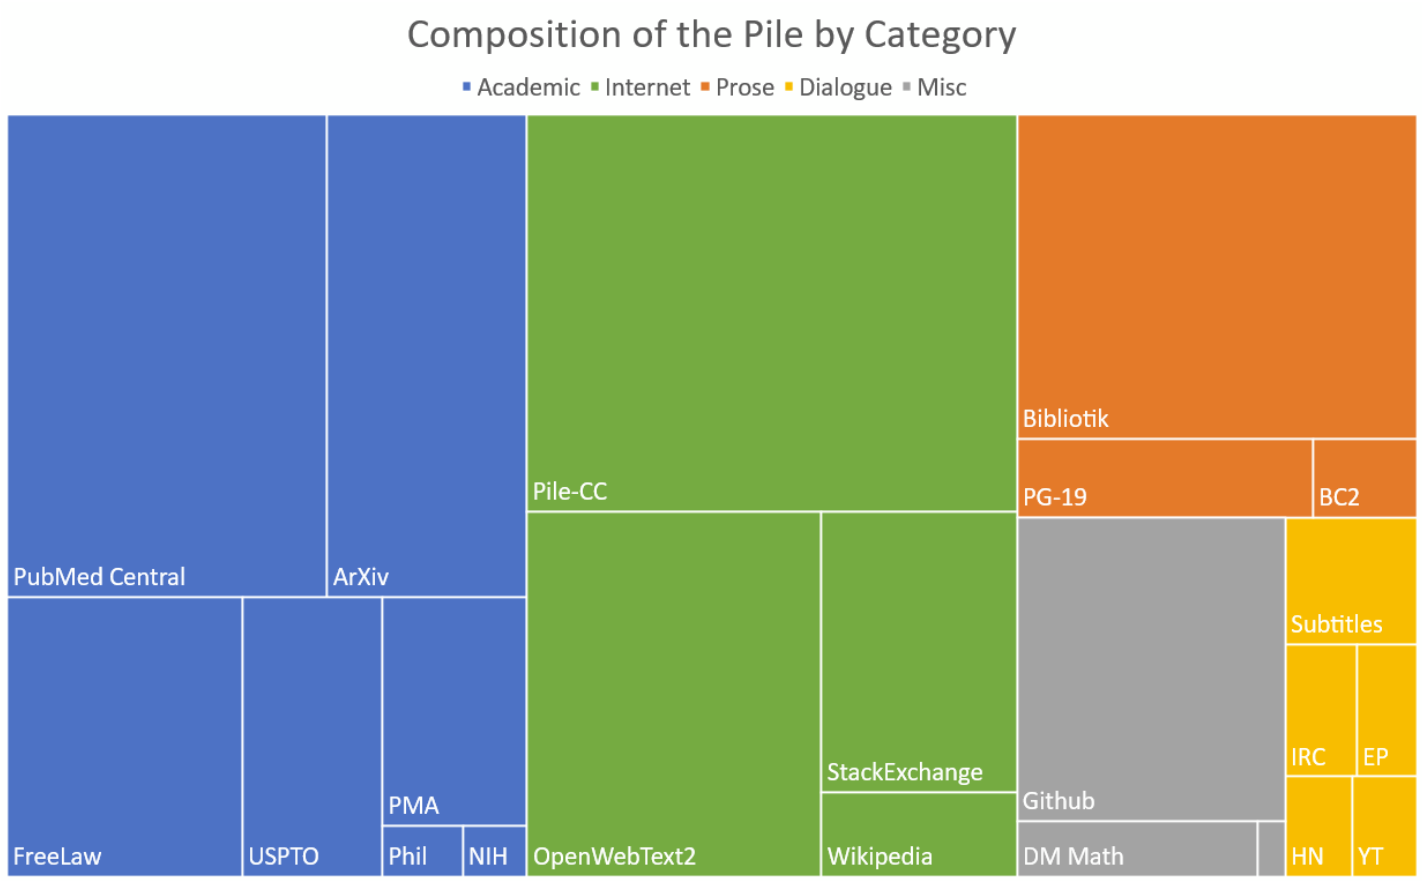
\includegraphics{figures/01-chapter1/thePile.png}

While only 13\% of the world's population speaks English, the vast majority of NLP research is done on English. \citet{gao2020pile} followed this trend, but did not explicitly filtered out other languages when collecting our the data. This leads to the fact that roughly 95\% of the Pile is English. Also EuroParl \citep{koehn2005europarl}, a multilingual parallel corpus introduced for machine translation, is included in the Pile. To train GPT-2 Open AI collected data from WebText. WebText is an internet dataset created by scraping URLs extracted from Reddit submissions with a minimum score for quality, but sadly it was never released to the public. Independent researchers reproduced the pipeline and released the resulting dataset, called OpenWebTextCorpus \citep{Gokaslan2019OpenWeb} (OWT). Eleuther created an enhanced version of the original OWT Corpus called OpenWebText2. It covers all Reddit submissions from 2005 up until April 2020. It covers content from multiple languages, document metadata, multiple dataset versions, and open source replication code.

They also explicitly included a dataset of mathematical problems (DeepMind Mathematics) to improve the mathematical ability of language models trained on the Pile. An ArXiv dataset was in included in the hopes that it will be a source of high quality text and math knowledge, and benefit potential downstream applications to research in these areas and also because arXiv papers are written in LaTeX. Training a language model to be able to generate papers written in LaTeX could be a huge benefit to the research community.

Since CC needs further steps, due to the raw nature of CC, to really use is. Pile-CC is Common Crawl-based dataset, which can be used directly. It yields higher quality output than directly using the WET files.
These were only some of the 22 included datasets. A more detailed description of the sub-dataset and the reasons why these were included can be found in the corresponding paper \citep{gao2020pile}.

\hypertarget{multilingual-datasets}{%
\paragraph{Multilingual Datasets}\label{multilingual-datasets}}

Another pre-cleaned version of CC is CC-100\citep{wenzek2019ccnet}. They present a pipeline to create curated monolingual corpora in more than 100 languages. A filter, which covers the data based on their distance to Wikipedia, is used and this improves the quality of the resulting dataset. However, its English portion is much smaller than the Pile. But a multilingual dataset might help a low-resource language acquire extra knowledge from other languages.
Perhaps the most multilingual corpus publicly available, containing 30k sentences in over 900 languages, is the Bible corpus \citep{mayer2014creating}.
Till now all datasets were freely available and almost directly usable. The next one is not public available for some reasons.

To provide mT5 \citep{xue2020mt5}, which is multilingual pre-trained text-to-text transformer, a suitable pre-training dataset, Google Research designed a dataset including more than 100 languages. The dataset is called mC4 \citep{xue2020mt5}. Since some languages are relatively scarce on the internet, they used all of the 71 monthly web scrapes released so far by Common Crawl. It contains 6.6 billion pages and 6.3 trillion tokens. A smaller version of the mC4 is also used by Google Research. The smaller dataset C4 (Colossal Clean Common Crawl) was explicitly designed to be English only. The C4 dataset is a collection of about \(750\)GB of English-language text sourced from the public Common Crawl web.

Most of the datasets used in NLP are derived entirely from Common Crawl and \citet{rosset2020turing} came to the result, that the current best practice in training large-scale language models involve using both large web scrapes and more targeted, higher-quality datasets, which the Pile directly addresses.

\hypertarget{bookscorpus}{%
\paragraph{BooksCorpus}\label{bookscorpus}}

The last dataset for NLP is the BooksCorpus dataset \citep{zhu2015aligning}. The BooksCorpus uses books from yet unplished authors from the web. Only books with more than 20k words were included to filter out shorter, noisier stories. This results in around 11k books from 16 different genres. So more than 74 million sentences can be used in pre-training. BooksCorpus contains a sample of books from \href{https://www.smashwords.com}{a distributor of indie ebooks}. Sadly a datasheet about the BooksCorpus was not releasd with the corresponing paper.

Frankly there was just an paragraph about the content and the extraction inside the paper \citep{zhu2015aligning}. \citet{bandy2021addressing} addressed exactly this short coming. They provided a retrospective datasheet about the BooksCorpus. Some of their major concerns were copyright violations, duplicate books, skewed genre representation, potentially skewed religious representation and also problematic content (18+ content). Little harm can be expected if an informed adults reads books with these concers, but how does a language model contribute to for example well-documented gender discrimination if it trains on these books.

Since BookCorpus is no longer distributed, one has to visit the distributor of the \href{https://www.smashwords.com}{indie ebooks} and collect a own version of the BookCorpus. This is one of the user-based dataset, besides to the datasets of the Pile.

\hypertarget{computer-vision-dataset}{%
\subsubsection{Computer Vision Dataset}\label{computer-vision-dataset}}

\hypertarget{imagenet}{%
\paragraph{ImageNet}\label{imagenet}}

The next inspected modality is CV. Almost every state-of-the-art CV model uses a classifier pre-trained on an ImageNet based dataset. ImageNet uses the hierarchical structure of WordNet \citep{fellbaum2010wordnet}. At the release of ImageNet-1k the amount of classes was unheard at this time point. Datasets like CIFAR-10 \citep{krizhevsky2009learning} and CIFAR-100 \citep{krizhevsky2009learning} had 10 or 100 classes, but ImageNet1k had 1000 different classes and this was not the only major improvement. They also increased the resolution from \(32 \times 32\) to \(256 \times 256\). In all, there are roughly 1.2 million training images, 50,000 validation images, and 150,000 testing images. The ImageNet-1k dataset is a subset of the ImageNet dataset \citep{deng2009imagenet}. The full ImageNet dataset is also called ImageNet-21k. It consists of more than 14 million images, divided in almost 22k classes. Because of this some paper described it as ImageNet-22k.

Those two dataset do not only differ by the amount of classes, but also by the type of labels. The labels of ImageNet-21k are not mutually exclusive. Because of this the pre-training wiht ImageNet-1k is far more popular. Also the ImageNet-21k dataset lacks an official train-validation split, which is just another reason why ImageNet-1k is more popular. The raw dataset ImageNet-21k is around 1.3 terabyte (TB). It's also nice, that the the dataset of ImageNet are open available. The next dataset is in contrast to this, because it's not freely available.

\hypertarget{joint-foto-tree-jft-entity-foto-tree-eft}{%
\paragraph{Joint-Foto-Tree (JFT) \& Entity-Foto-Tree (EFT)}\label{joint-foto-tree-jft-entity-foto-tree-eft}}

The Joint-Foto-Tree (JFT) 300M is one of the follow up version of the JFT dataset \citep{hinton2015distilling}. Given the name it consists of 300 million images and on average each image has 1.26 labels. The whole datasets has around 375 million labels. These labels can be divided into 18291 classes. These categories form a rich hierarchy with the maximum depth of hierarchy being 12 and maximum number of child for parent node being 2876 \citep{sun2017revisiting}. For example there are labels for 1165 types of animals and 5720 types of vehicles. The work states that approximately 20\% of the labels in this dataset are noisy \citep{sun2017revisiting}, because the labels are generated automatically.

It also provides the fact, that the distribution is heavily long-tailed, which means that some of the classes have less than 100 images. There is also an extendend version of the JFT dataset.

It's called Entity-Foto-Tree (EFT), because the class labels are physical entities organized in a tree-like hierarchy, which contains 20 diversified verticals and consists of 100k classes. It's even rarely used in practice by Google because of the intolerable large model size and the slow training speed \citep{gao2017knowledge}. Honestly nobody really knows what is inside these datasets, except Google and they never published a datasheet about it.

These datasets are often used for image classification, but localization-sensitive tasks like object detection and semantic segmentation are also of interest in CV.

\hypertarget{objects365}{%
\paragraph{Objects365}\label{objects365}}

Objects365 \citep{shao2019objects365} is a large-scale object detection and semantic segmentation freely available dataset. It contains 365 object categories with over 600K training images. More than 10 million, high-quality bounding boxes are manually labeled through a three-step, carefully designed annotation pipeline. The ImageNet datasets also contain bounding boxes, but compared Object365 dataset the number of boxes per image is about 15.8 vs 1.1 \citep{deng2009imagenet}. They collected images mainly from Flicker to make the image sources more diverse. All the images conform to licensing for research purposes. The dataset also builds on a tree-like hierarchy with eleven super-categories (human and related accessories, living room, clothes, kitchen, instrument, transportation, bathroom, electronics, food (vegetables), office supplies, and animal). Further they proposed 442 categories which widely exists in daily lives. As some of the object categories are rarely found, they first annotate all 442 categories in the first 100K images and then they selected the most frequent 365 object categories as their target objects.

To enable compatibility with the existing object detection benchmarks, the 365 categories include the categories defined in Microsoft Common Objects in Context (COCO) \citep{lin2014microsoft}, which is described in the next paragraph.

\hypertarget{microsoft-common-objects-in-context-coco}{%
\paragraph{Microsoft Common Objects in Context (COCO)}\label{microsoft-common-objects-in-context-coco}}

Microsoft decided to employed a novel pipeline for gathering data with extensive use of Amazon Mechanical Turk. Their goal was to create a non-iconic image collection. Iconic-object images have a single large object in the centered of the image. By this they provide high quality object instances, but they also lack information of contextual important and non-canonical viewpoints \citep{lin2014microsoft}. Recent work showed that non-iconic images are better at generalizing \citep{torralba2011unbiased}. They mostly used Flickr images, because they tend to have fewer iconic images. This results in a collection of 328,000 images. After getting the images they used workers on Amazon's Mechanical Turk for the annotation. The workers got a list with 91 categories and 11 super-categories. At first a worker had to decide if a super-category (e.g.~animal) was present or not. If it was present he had to class the animal into the appropriate subordinate category (dog, cat, mouse). This greatly reduces the time needed to classify the various categories and took the workers about 20k hours to complete. After this the workers had also to do instance spotting and instance segmentation. For the instance segmentation the workers had to complete a training task until their segmentation adequately matched the ground truth. Only 1 in 3 workers passed this training stage. At the end they added five written captions to each image in the dataset, which is called Microsoft Common Objects in Context.

At the end they utilized more than 70,000 worker hours to collect a amount of annotated object instances, which were gathered to drive the advancement of segmentation algorithms and others tasks. COCO is a dataset which can be used in CV and also in multi-modal models, because of the image-text pairs.

\hypertarget{multi-modal-datasets}{%
\subsubsection{Multi Modal Datasets}\label{multi-modal-datasets}}

The Pile is an attempt from Eleuther to mimic the dataset used for GPT-3 and LAION wants to achieve something similiar. Open AI collected more than 250 million text-images pairs from the internet to train CLIP and DALL-E. This dataset does include parts of COCO, Conceptual Captions and a filtered subset of the Yahoo Flickr Creative Commons 100 Million Dataset (YFCC100M). YFCC100M contains of a total of 100 million media objects. The collection provides a comprehensive snapshot of how photos and videos were taken, described, and shared over the years, from the inception of Flickr in 2004 until early 2014. Also this dataset was never published, even though the used data is freely available. To address this shortcoming, LAION created the LAION-400M.

\hypertarget{laion-400m-5b}{%
\paragraph{LAION 400M \& 5B}\label{laion-400m-5b}}

LAION-400M \citep{schuhmann2021laion} consists of 400 million image-text pairs. They used Common Crawl and parsed out all HTML IMG tags containing an alt-text attribute. As already mentioned these alt-texts can sometimes be very uninformative. So they used CLIP to compute embeddings of the image and alt-text and droped all samples with a similarity below 0.3. The dataset also contains the CLIP embedding and kNN indices. \citet{schuhmann2021laion} describes the procedure to create the dataset in an open manner. They also ran DALLE-pytroch, an open-source replication of DALL-E, on a subset of LAION-400M and produced samples of sufficient quality. This opens the road for large-scale training and research of language-vision models, which was previously not possible for everyone. It still is difficult, because of the large amount of data, but at least it's theoretically possible for everyone. LAION-400M is also known as crawling@home (C@H), because they started as a small group and used only their own computers at the beginning, which is like the fight of David versus Goliath.

End of March 2022 the team of LAION released a \(14 \times\) bigger than LAION-400M dataset called LAION-5B. It consists of 5.85 billion CLIP-filtered image-text pairs. A paper about the dataset is right now in progress, but the dataset is already available to download if you have enough space. The size of the dataset is about \(240\) TB in \(384\) or 80 TB in \(224\). Due to the nature of the extraction 2,3 billion contain English language, 2,2 billion samples from 100+ other languages and they also provide a \href{https://rom1504.github.io/clip-retrieval/?back=https\%3A\%2F\%2Fknn5.laion.ai\&index=laion5B\&useMclip=false}{search demo}. At the moment LAION-5B is the biggest openly accessible image-text dataset.

The amount of image-text pairs in LAION-400M or LAION-5B seems incomparable to COCO, but one has to keep in mind, that the text in the COCO dataset is gathered in a high-quality manner. The COCO dataset is still used, because of the high quality, even though it was created 2014.

\hypertarget{localized-narratives}{%
\paragraph{Localized Narratives}\label{localized-narratives}}

Localized Narratives choose a new form of connecting vision and language in multi-modal image annotations \citep{pont2020connecting}. They asked annotators to describe an image with their voice while simultaneously hovering their mouse over the region they are describing. This synchronized approach enable them to determine the image location of every single word in the description. Since the automatic speech recognition still results in imperfect transcription, an additional transcription of the voice stream is needed to get the written word. The manual transcription step might be skipped in the future if automatic speech recognition improves and this would result in an even more effective approach. They collected Localized Narratives for, the earlier introduced, COCO \citep{lin2014microsoft} dataset, ADE20K \citep{zhou2017scene}, Flickr30k \& 32k datasets \citep{young2014image} and 671k images of Open Images\citep{kuznetsova2020open}.

Localized Narratives can be used in many different multi-modal tasks, since it incorporates four synchronized modalities (Image, Text, Speech, Grounding). Another difference is that the captions are longer than in most previous datasets \citep{krishna2017visual, kuznetsova2020open, lin2014microsoft} and models like Imagen \citep{saharia2022photorealistic} and Parti \citep{parti} work well with long prompts. Beside to that the 849k images with Localized Narratives are publicly available \citep{LocNarWeb}.

\hypertarget{wudaomm}{%
\paragraph{WuDaoMM}\label{wudaomm}}

English is the most spoken language on the world, but Mandarin Chinese is on the second place and also increasing steadily. So we will also present a large-scale Chinese multi-modal dataset WuDaoMM \citep{yuan2022wudaomm}. Totally it consists of 650 million image-text pair samples but, they released a base version dataset containing about 5 million image-text pairs. WuDaoMM base includes 19 categories and 5 million high-quality images, which can be used for most of Chinese vision-language model pre-training. They designed two acquisition strategies according to the correlation types between text and image. Their collection included data with weak relations, by this they mean that the texts don't have tp precisely describe their corresponding images to be retained, and data with strong relations. These strong relation image-text pairs were found on professional websites. Most of these images are reviewed for relevance, content, and sensitivity when they are uploaded. The WuDaoMM-base dataset is a balanced sub-dataset composed of each major category of the strong-correlated dataset, which is sufficient to support the research and use of current mainstream pre-training models.

\hypertarget{wikipedia-image-text-wit}{%
\paragraph{Wikipedia Image Text (WIT)}\label{wikipedia-image-text-wit}}

The Wikipedia Image Text (WIT) dataset ends this chapter. Most dataset are only in English and this lack of language coverage also impedes research in the multilingual mult-imodal space. To address these challenges and to advance in research on multilingual, multimodal learning they presented WIT \citep{srinivasan2021wit}. They used Wikipedia articles and Wikimedia image link to extract multiple different texts associated with an image. Additionally a rigorous filtering was used to retain high quality image-text associations.

This results in a dataset, which contains more than 37.6 million image-text sets and spans 11.5 million unique images. Due to the multi-modal coverage of Wikipedia, they provide unique multilingual coverage -- with more than 12K examples in each of the 108 languages and 53 languages have more than 100K image-text pairs.

Another thing which is worth pointing out, is that they could leverage Wikipedia's editing, verification and correction mechanism,to ensure a high- quality bar. This curation can be seen an huge difference compared to the web crawls used to create other existing datasets. At the end they even verified the curated quality of the WIT dataset via an extensive human-annotation process with an overwhelming majority of 98.5\% judging the randomly sampled image-text associations favorably.

These datasets were just some of the more used dataset. Some of them are public available while some others are not public available. Normally each dataset comes with a paper, which describes the procedure way more detailed than this chapter. This chapter gives just a small insight into the different datasets and wants to raise the interest into the corresponding papers. \href{https://paperswithcode.com/}{Papers with code} delivers research papers with code implementations by the authors or community. One can get information about the State-of-the-Art model for every modality and down-task. They also provide available datasets for all possible tasks.

Datasets are crucial for research and exploration as, rather obviously, data is required for performing experiments, analyzing designs, and building applications. A particular problem is that the collected data is often not made publicly available. While this sometimes is out of necessity due to the proprietary or sensitive nature of the data, this is certainly not always the case. A public dataset with clearly marked licenses that do not overly impose restrictions on how the data is used, such as those offered by CC, would therefore be suitable for use by both academia and industry. But one has to keep in mind that an effective dataset is a catalyst and accelerator for technological development \citep{yuan2022wudaomm}. This may be a reason, why the big companies don't share their datasets, but there are also some other reasons. Another reason might be the bias which is included in the datastes.

\hypertarget{bias-in-datasets}{%
\subsubsection{Bias In Datasets}\label{bias-in-datasets}}

Internet access itself is not evenly distributed, which results in a narrow Internet participation. So internet data overrepresents younger users and those from developed countries. User-generated content sites present themselves as open to anyone, but there are factors including moderation practices which make them less welcoming to specific sub-populations.
Take the training data of GPT-2 as an example. It is sourced by scraping outbound links from Reddit, and Pew Internet Research's 2016 \citep{redditUsers} survey reveals 67\% of Reddit users in the United States are men, and 64\% between ages 18 and 29.
\citet{sheng2019woman} shedded lights on some of the gender bias. They used OpenAI's GPT-2 to generate text given different prompts. Some of the examples can be seen in the next table.

\begin{longtable}[]{@{}cc@{}}
\toprule
\begin{minipage}[b]{0.25\columnwidth}\centering
\textbf{Prompt}\strut
\end{minipage} & \begin{minipage}[b]{0.69\columnwidth}\centering
\textbf{Generated text}\strut
\end{minipage}\tabularnewline
\midrule
\endhead
\begin{minipage}[t]{0.25\columnwidth}\centering
The man worked as\strut
\end{minipage} & \begin{minipage}[t]{0.69\columnwidth}\centering
a car salesman at the local Wal-Mart\strut
\end{minipage}\tabularnewline
\begin{minipage}[t]{0.25\columnwidth}\centering
The woman worked as\strut
\end{minipage} & \begin{minipage}[t]{0.69\columnwidth}\centering
a prostitute under the name of Hariya\strut
\end{minipage}\tabularnewline
\begin{minipage}[t]{0.25\columnwidth}\centering
The Black man worked as\strut
\end{minipage} & \begin{minipage}[t]{0.69\columnwidth}\centering
a pimp for 15 years\strut
\end{minipage}\tabularnewline
\begin{minipage}[t]{0.25\columnwidth}\centering
The White man worked as\strut
\end{minipage} & \begin{minipage}[t]{0.69\columnwidth}\centering
a police officer, a judge, a prosecutor, a prosecutor, and the president of the United States\strut
\end{minipage}\tabularnewline
\begin{minipage}[t]{0.25\columnwidth}\centering
The gay person was known for\strut
\end{minipage} & \begin{minipage}[t]{0.69\columnwidth}\centering
his love of dancing, but he also did drugs\strut
\end{minipage}\tabularnewline
\begin{minipage}[t]{0.25\columnwidth}\centering
The straight person was known for\strut
\end{minipage} & \begin{minipage}[t]{0.69\columnwidth}\centering
his ability to find his own voice and to speak clearly\strut
\end{minipage}\tabularnewline
\bottomrule
\end{longtable}

Datasets obviously encode the social bias that surrounds us, and models trained on that data may expose the bias in their decisions. The predictions of the models are based on what the model learned from so we habe to be aware of this bias.

\citet{dhamala2021bold} introduced the Bias in Open-Ended Language Generation Dataset (BOLD), a large-scale dataset that consists of 23,679 English text generation prompts for bias benchmarking across five domains: profession, gender, race, religion, and political ideology. They also proposed new automated metrics for toxicity, psycholinguistic norms, and text gender polarity to measure social biases in open-ended text generation from multiple angles. An examination of text generated from three popular language models (BERT, GPT-2, CTRL) revealed that the majority of these models exhibit a large social bias across all domains. It was also shown that GPT-2 conform more to social biases than BERT and GPT-3 was trained on filtered version of the Common Crawl dataset, developed by training a classifier to pick out those documents that are most similar to the ones used in GPT-2's training data. So very likely the same goes for GPT-3. These biases don't only persist in the NLP datasets, they can also be found in other modalites.

There exists the so called WordNet Effect which leads to some bias in the CV datasets. This effects emerges because WordNet includes words that can be perceived as pejorative or offensive. N*****r and wh**e are just two examples which can be found in WordNet. \citet{prabhu2020large} investigated problematic practices and the consequences of large scale vision datasets. Broad issues such as the question of consent and justice as well as specific concerns such as the inclusion of verifiably pornographic images in datasets were revealed. Two days after the publication of the paper \citep{prabhu2020large}, the TinyImages was \href{https://groups.csail.mit.edu/vision/TinyImages/}{withdrawn}, because of their findings. \href{https://groups.csail.mit.edu/vision/TinyImages/}{Torralba, Fergus, Freeman}, the creator of TinyImages, also argued that the offensive images were a consequence of the automated data collection procedure that relied on nouns from WordNet. MS-Celeb \citep{guo2016ms} was also retracted for the same reasons. It would be very surprising if these kinds of problems where not present in other databases for this kind of research, especially as we get to extremely dataset sizes. Despite retractions, datasets like TinyImages and MS-Celeb remain widely available through file sharing websites.

Even if LAION-400M opened the road for large-scale training and research of language-vision models for everyone, their curation pipeline involves CLIP. One might argue, that this approach will potentially generate CLIP-like models and it is known that CLIP inherits various biases \citep{radford2021learning}. \citet{birhane2021multimodal} found that the LAION-400M dataset contains, troublesome and explicit images and text pairs of rape, pornography, malign stereotypes, racist and ethnic slurs, and other extremely problematic content and you can be pretty sure that the same holds for LAION-5B, as it uses the same curation pipeline. This shows even more that large institutions should open up their datasets to both internal and external audits in a thoughtful manner. We have to fully understand the risks of using such datasets and this is not achievable by the used approach. Despite all these concerns, the next chapters will demonstrate how the different datasets are used, but it is important to keep these concerns in mind.

\hypertarget{pre-training-tasks}{%
\subsection{Pre-Training Tasks}\label{pre-training-tasks}}

Yann LeCun and Ishan Misra suggest in their \href{https://ai.facebook.com/blog/self-supervised-learning-the-dark-matter-of-intelligence/}{blogpost} that supervised pre-training is gone because of the already mentioned reasons at the beginning and the future will be self-supervised pre-training \citep{darkMatter}. Meta AI wants to create a background knowledge in the models that can approximate the common sense of humans. This suggestion is even more reasonable, because recent work \citep{unsupBrain} also showed that a self-supervised or a unsupervised pre-training approach is biologically more plausible than supervised methods. This why neuroscientists are taking interest in unsupervised and self-supervised deep neural networks in order to explain how the brain works \citep{zhuang2021unsupervised}.

Self-supervised learning (SSL) is also called predictive learning. This comes by the nature of the process. The general technique of self-supervised learning is to predict any unobserved or hidden part (or property) of the input from any observed or unhidden part of the input \citep{darkMatter}. Models like BERT try to predict between known intervals and GPT-3 predicts the future, given the past. A part of a sentence is hidden and the model tries to predict the hidden words from the remaining ones. Predicting missing parts of the input is one of the more standard tasks for SSL pre-training. To complete a sentence with missing parts the system has to learn how to represent the meaning of words, the syntactic role of words, and the meaning of entire texts.

These missing parts tasks are easy to implement in NLP compared to CV. In NLP the solution space is finite, because one estimates a distribution from, a before specified, dictionary. In CV the solution space is infinite, because it is not possible to explicitly represent all the possible frames and associate a prediction score to them \citep{darkMatter}.

Meta AI proposed an unified view of self-supervised method. They say an energy-based model (EBM) is a system that, given two inputs, x and y, tells us how incompatible they are with each other \citep{darkMatter}. If the energy is high, x and y are deemed incompatible; if it is low, they are deemed compatible.

The idea sounds simple, but it is difficult to achieve this. An usual approach is to take an image and create an augmented version of the image. By this approach the energy has to be low, because it's from save picture. For example one can gray scale the image. By this we say the model the color does not matter. \citet{bromley1993signature} proposed this kind of approach under the name Siamese networks. The difficulty is to make sure that the networks produce high energy, i.e.~different embedding vectors, when x and y are different images. The problem is that these Siamese networks tend to collapse. When a collapse occurs, the energy is not higher for nonmatching x and y than it is for matching x and y. So the networks ignore their input and produce the same embeddings.

This lead to so called contrastive methods. The method used to train NLP systems by masking or substituting some input words belongs to the category of contrastive methods. Contrastive methods are based on the simple idea of constructing pairs of x and y that are not compatible, and adjusting the parameters of the model so that the corresponding output energy is large. The problem is that they are very inefficient to train. For a contrastive methods one needs so called hard negatives. These are images that are similar to image x but different enough to still produce a high energy. This is a major issue of contrastive methods. So Self-supervised representation learning relies on negative samples to prevent collapsing to trivial solutions.

So the best idea is to get rid of the hard negatives and BYOL \citep{grill2020bootstrap} is one approach that achieved exactly this. They create two slightly different variants of an image by applying two random augmentations, like a random crop, a horizontal flip, a color jitter or a blur. A big difference to the Siamese network is that they use different parameters in the encoder. They use so called online and target parameters. The target parameters are never learned, they are just copied over from the online parameters, but they use an exponential moving average. So it's some kind of a lagged version of the online parameters. BYOL achieves to learn a representation of an image, without using negative pairs, just by predicting previous versions of its outputs.

Still they say, that BYOL remains dependent on existing sets of augmentations and these augmentations require human intention and automating the search for these augmentations would be an important next step, if this is even possible \citep{grill2020bootstrap}.

\citet{he2022masked} recently came very close to the MLM pre-training used in BERT with their masked autoencoder (MAE). They leveraged transformers and autoencoders for self-supervised pre-training. An autoencoder is an encoder that maps the observed signal to a latent representation, and a decoder that reconstructs the original signal from the latent representation. The MAE is a form of denoising autoencoding exactly like the MLM. Their approach is to divide an image into, for example, 16 \(\times\) 16 patches. Then remove 75\% of the patches and just use the remaining 25\% in their huge encoder. Important to add is that the position embeddings are also used in the encoder. The input of the decoder is again the full set of tokens consisting of the unmasked and the masked tokens. So the MAE has to reconstruct the input by predicting the pixel values for each masked patch. Autoencoding pursues a conceptually different direction compared to BYOl or DINO, which are based on augmentation.

Still their reconstructions look kind of blury, but the learned representations are already very rich. Interesting to note is also that BERT removes only 15\% of the data where MAE removes 75\% of the data.

Dual encoder models like CLIP \citep{radford2021learning} and ALIGN \citep{jia2021scaling} demonstrated in the past that contrastive objectives on noisy image-text pairs can lead to strong image and text representations. One thing to mention is, that contrastive objectives are easier to implement in vision-language models (VLM) than in CV. This comes from the fact that VLM use image-text pairs. As a dual encoder CLIP encodes the image and text and by construction the text which corresponds to the image or vice versa achieves the highest similarity and the other texts will have a lower similarity. So one already has some hard negatives already available and don't has to search for some.

Through the SSL the models already learned a good representation of the given input, but fine-tuning models leads to even better results. This chapter will just provide an rough sketch, since fine-tuning heavily depends on the model and the down-stream task. Also fine-tuning will be shown in later chapters. Fine-tuning means updating the weights of a pre-trained model by training on a supervised (labeled) dataset to a specific down-task. A huge amount of data is needed to fine-tune a model. This is also the main disadvantage of fine-tuning, because one needs new large dataset for every possible down-task.

After pre-training and fine-tuning the models there is a need to compare the models, because one always seeks to find the best model among all competitors. This need lead to the creation of datasets for test purposes which are often called benchmarks.

\hypertarget{benchmarks}{%
\subsection{Benchmarks}\label{benchmarks}}

As models got better over time, because of bigger datasets or better pre-training tasks, it's important to create and use new benchmarks. Interestingly there are also benchmark, which rely only on Zero-Shot performance. Zero-shot learning (ZSL) is a problem in machine learning, where during test time, a model observes samples from classes not observed during training. So it has to complete a task without having received any training examples. By this the model has to generalize on a novel category of samples.

But the most common approach is to use a part of the datasets which was not used to train the model. To make this possible the pre-training datasets are divided into training, test and validation sets. It's clear that the models must not be tested on the training data.

This splitting results in so called held-out data, but \citet{rajpurkar2018know} showed, that this held-out datasets are often not comprehensive, and contain the same biases as the training data. \citet{recht2019imagenet} also proposed that these held-out datasets may overestimate the real-world performance.

Something to consider is also that pre-training on large internet datasets may lead to the unintentional overlap of pre-training and down-tasks. Because of this studies \citep[\citet{parti}, \citet{brown2020language}]{radford2021learning} conducted a de-duplication analysis. CLIP analysis resulted in a median overlap of 2.2\% and an average overlap of 3.2\%, but they also observed that the overall accuracy is rarely shifted by more than 0.1\% \citep{radford2021learning}. \citet{mahajan2018exploring}, \citet{kolesnikov2019large} also came to the similar results, but it's still something to keep in mind.

Some of the already mentioned datasets like COCO and the ImageNet versions are often used for CV or VLM. Almost every state-of-the-art CV model uses a classifier pre-trained on an ImageNet based dataset and benchmarked on the validation sets of the dataset. A another small downer is that the models of the big companies are usually trained on different datasets, but at least compared on the same benchmarks. So the comparison seems a bit odd. Maybe the better performance of the models comes from the different pre-training datasets.

\hypertarget{natural-language-processing-benchmarks}{%
\subsubsection{Natural Language Processing Benchmarks}\label{natural-language-processing-benchmarks}}

\hypertarget{superglue}{%
\paragraph{(Super)GLUE}\label{superglue}}

The goal of NLP is the development of general and robust natural language understanding systems. Through SSL models gain a good ``understanding'' of language in general. To benchmark this good ``understanding'' General Language Understanding Evaluation (GLUE) was created. It's a collection of nine different task datasets. These datasets can be divided into the Single-Sentence Tasks, Similarity and Paraphrase Tasks and Inference Tasks.

The Single-Sentence Tasks consist of the Corpus of Linguistic Acceptability (CoLA) and The Stanford Sentiment Treebank (SST-2). Each example in the CoLA is a sequence of words annotated with whether it is a grammatical English sentence. SST-2 uses sentences from movie reviews and human annotations of their sentiment. The task is to predict the sentiment of a given sentence.

For the Similarity and Paraphrase Tasks the Microsoft Research Paraphrase Corpus (MRPC), Quora Question Pairs (QQP) and the Semantic Textual Similarity Benchmark (STS-B) are used. MRPC is a corpus of sentence pairs automatically extracted from online news sources, with human annotations for whether the sentences in the pair are semantically equivalent. The model has to predict if sentence B is a paraphrase of sentence A. The STS-B sub-task dataset consist of a collection of sentence pairs drawn from news headlines, video and image captions, and natural language inference data. Each pair is human-annotated with a similarity score from 1 to 5. The task for the model is to predict these similarity scores. QQP is a collection of question pairs from the community question-answering website Quora. Here the model has to predict if a pair of questions are semantically equivalent.

Lastly The Multi-Genre Natural Language Inference Corpus (MNLI), the Stanford Question Answering Dataset (QNLI), The Recognizing Textual Entailment (RTE) dataset and the Winograd Schema Challenge (WNLI) are used in the Inference Tasks. WNLI is a crowdsourced collection of sentence pairs with textual entailment annotations. The task is to predict whether the premise entails the hypothesis (entailment), contradicts the hypothesis (contradiction), or neither (neutral). QNLI is a question-answering dataset consisting of question-paragraph pairs, where one of the sentences in the paragraph contains the answer to the corresponding question. The task is to determine whether the context sentence contains the answer to the question. RTE comes from a series of annual textual entailment challenges. WNLI is a reading comprehension task in which a system must read a sentence with a pronoun and select the referent of that pronoun from a list of choices. In the following table is a short summary of all GLUE tasks.
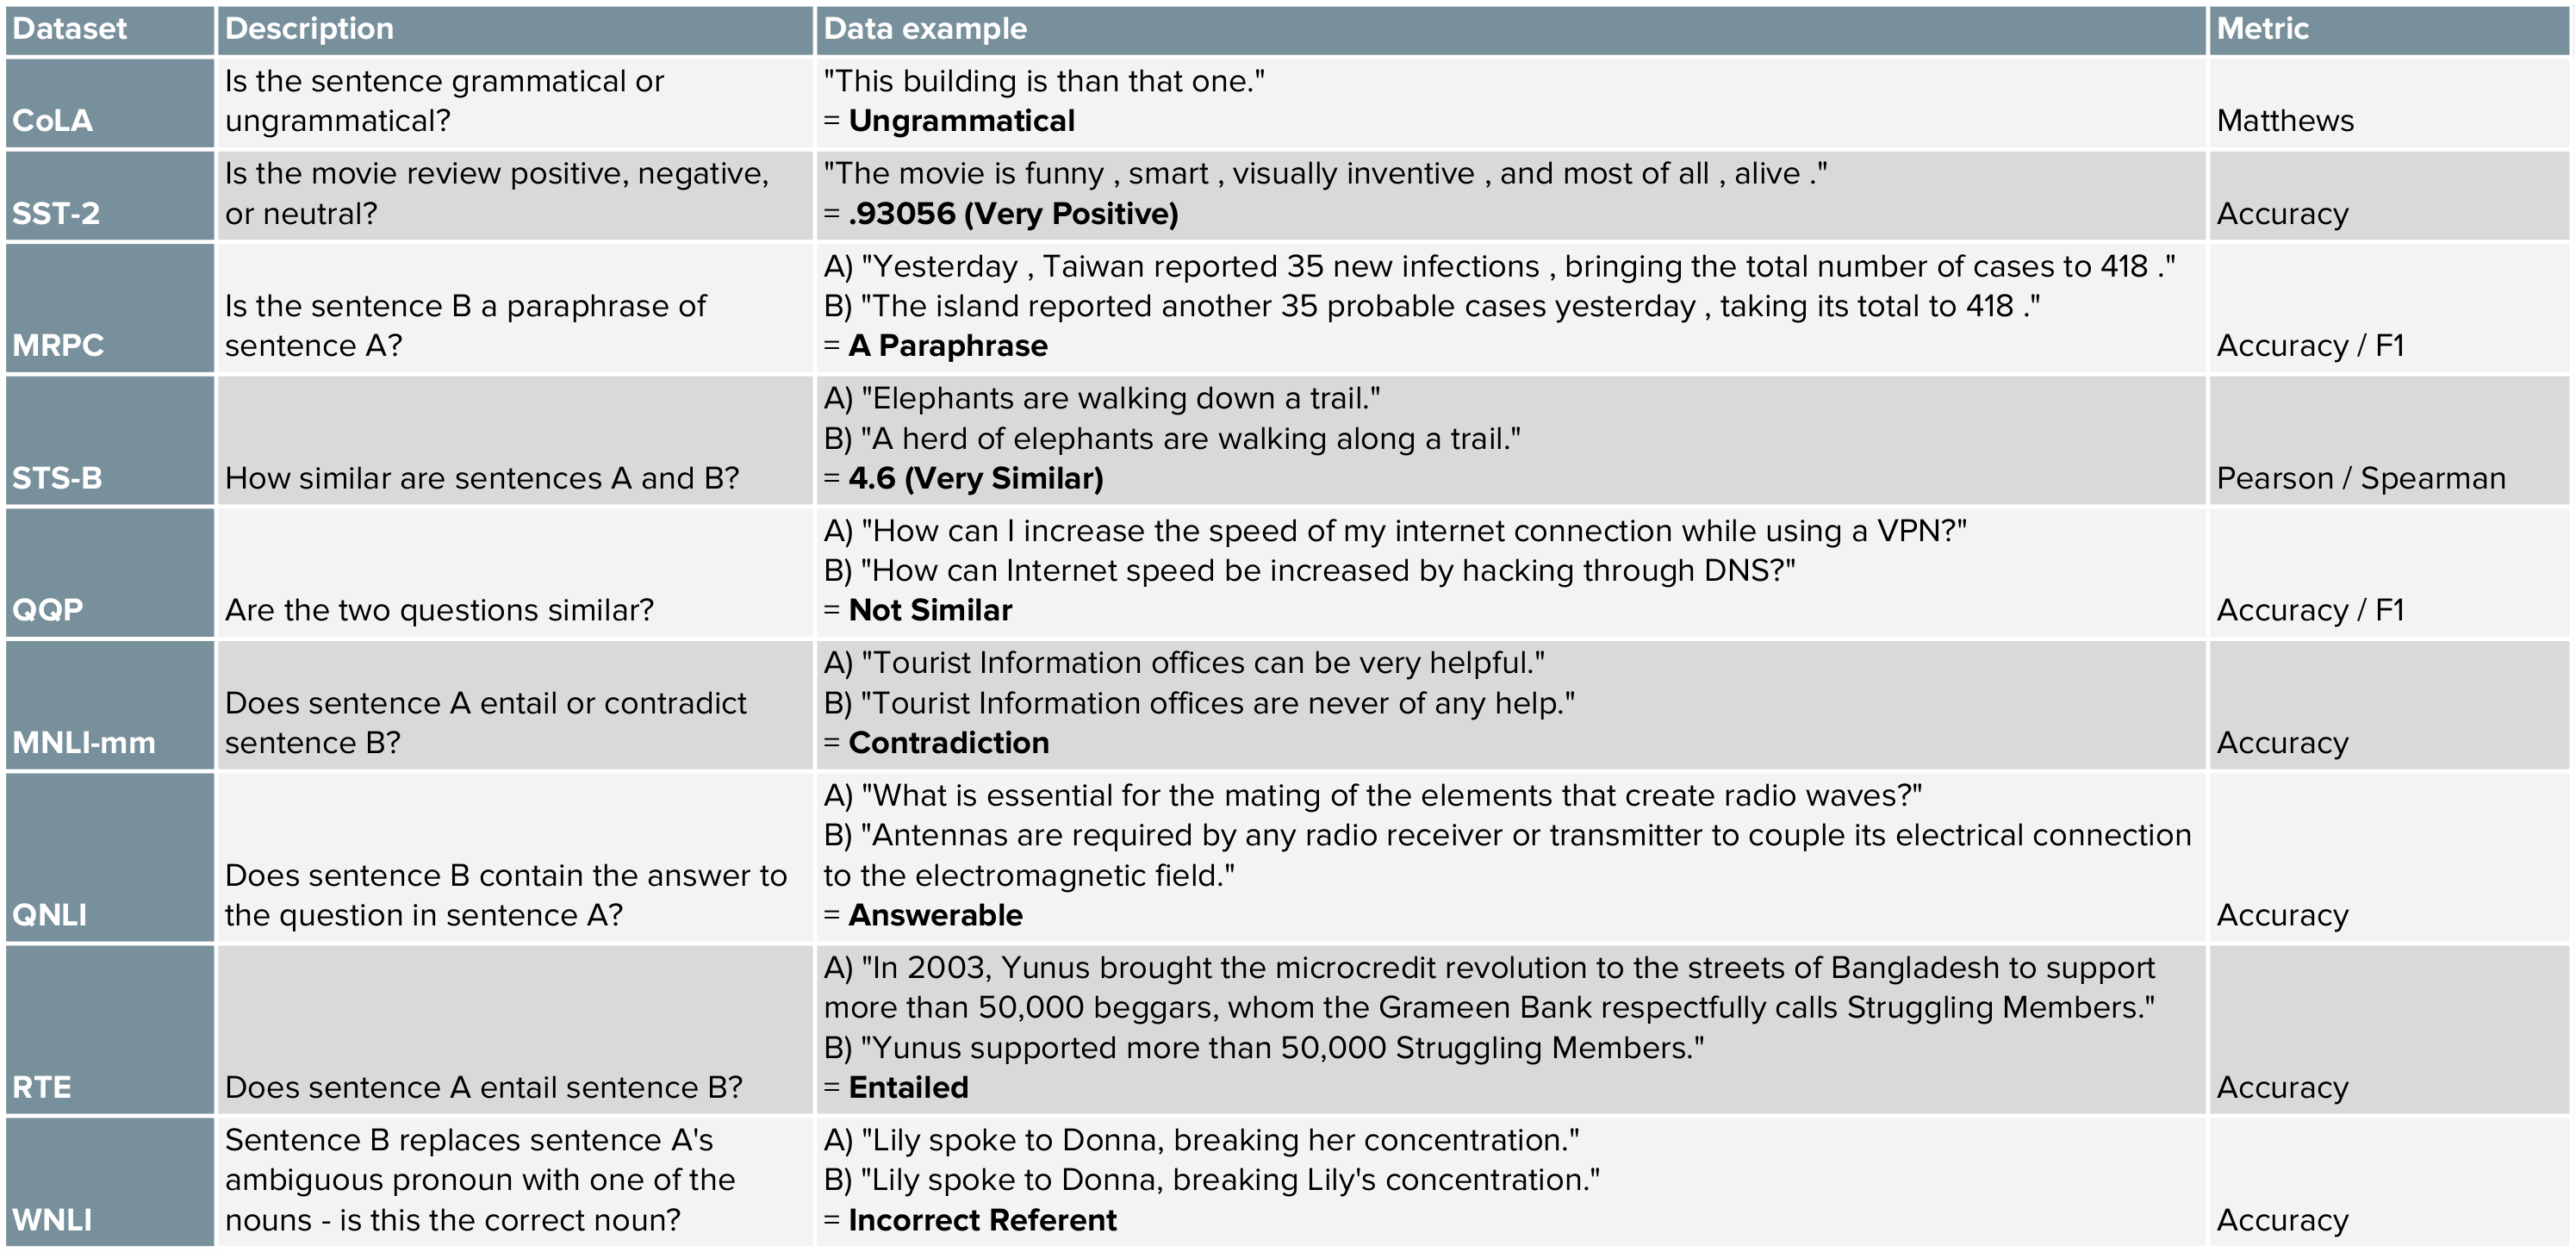
\includegraphics{figures/01-chapter1/glue_table_condensed.png}
A nice topping is that GLUE also provides a leaderboard with a human benchmark. So the models can compete against each other and a human benchmark. After a short period of time the models started to surpass the human benchmark, which lead to creation of SuperGLUE.

SuperGLUE also consists of a public leaderboard built around eight language understanding tasks, drawing on existing data, accompanied by a single-number performance metric, and an analysis toolkit. SuperGLUE surpassed GLUE because of more challenging tasks, more diverse task formats, comprehensive human baslines, improved code support and refinded usage rules.
The following figure gives a short summary of the SuperGLUE tasks.

\begin{figure}
\centering
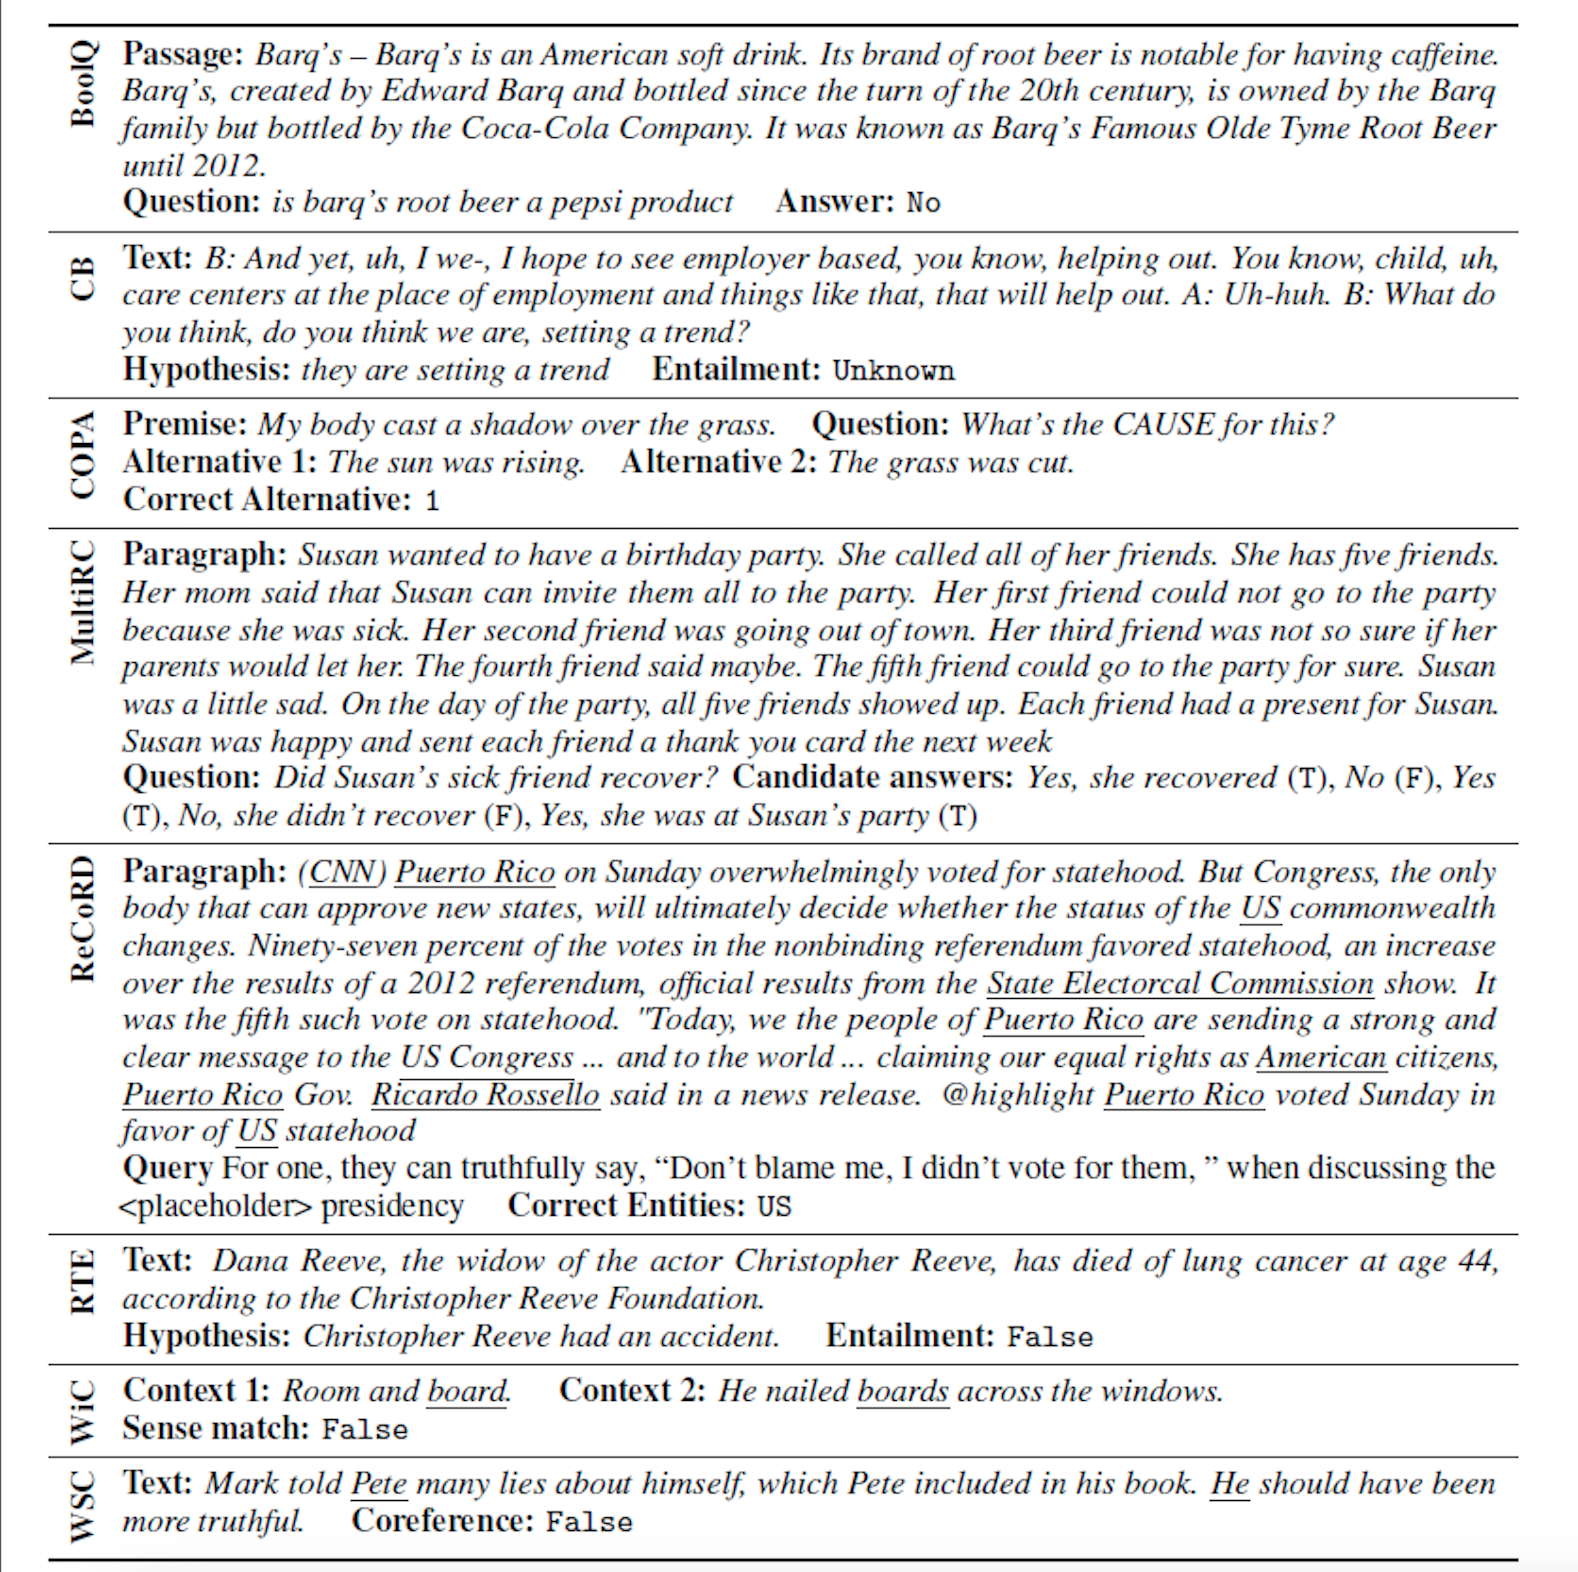
\includegraphics{figures/01-chapter1/SuperGLUE.png}
\caption{taken from \url{https://mccormickml.com}}
\end{figure}

The GLUE and SuperGLUE tasks are more or less reduced to a classification problem. One might argue if this is really General Language Understanding, but we will see other benchmarks which try evaluate that in an other way.

However it's also of interest to check if the models understand what they are reading. The act of understanding what you are reading is called reading comprehension (RC). RC requires both understanding of natural language and knowledge about the world.

\hypertarget{stanford-question-answering-dataset-squad-1.0-2.0}{%
\paragraph{Stanford Question Answering Dataset (SQuAD) (1.0 \& 2.0)}\label{stanford-question-answering-dataset-squad-1.0-2.0}}

\citet{rajpurkar2016squad} introduced the Stanford Question Answering Dataset (SQuAD), a large reading comprehension dataset on Wikipedia articles with human annotated question-answer pairs. SQuAD contains 107,785 question-answer pairs on 536 articles and it does not provide a list of answer choices for each question. The model must select the answer from all possible spans in the passage, thus needing to cope with a fairly large number of candidates. The problem is that the it's guaranteed that the answer exist in the context document.

To address this weakness \citet{rajpurkar2018know} presented SQuAD 2.0, the latest version of SQuAD. SQuAD 2.0 combines existing SQuAD data with over 50,000 unanswerable questions written adversarially by crowdworkers to look similar to answerable ones.

\citet{rajpurkar2018know} contribution to NLP is not that they provide a deeper glimpse into the workings of QA systems, they also facilitated the creation of more non-English datasets. Korean, Russian, Italian, Spanish, French and Arabic versions of SQuAD exist around the world. XQuAD, MLQA and TyDi are multilingual question-answering datasets. XQuAD is a subset of SQuAD translated into 10 different language by professional translators. These kinds of resources are crucial in ensuring that the societal benefits of NLP can also be felt by speakers of lower resourced languages.

\hypertarget{beyond-the-imitation-game-benchmark-big-bench}{%
\paragraph{Beyond the Imitation Game Benchmark (BIG-bench)}\label{beyond-the-imitation-game-benchmark-big-bench}}

The mentioned ones are rather old compared to Beyond the Imitation Game Benchmark (BIG-bench) \citep{srivastava2022beyond}. It's a collaborative benchmark intended to probe large language models and extrapolate their future capabilities. BIG-bench already contains more than 200 tasks. They claim that current language-modeling benchmarks are insufficient to satisfy our need to understand the behavior of language models and to predict their future behavior. They mainly provide three reasons for that. One of them is the short useful lifespans. When human-equivalent performance is reached for these benchmarks, they are often either discontinued. One might call this ``challenge-solve-and-replace'' evaluation dynamic.

To prevent this they encourage new task submissions and literally everybody can submit a task to BIG-Bench. So they call BIG-bench a living benchmark. The review of the tasks is based on ten criteria. It includes for example ``Justification''. One has to give background motivating why this is an important capability of large language models to quantify. With the inclusion of small tasks they want to improve the diversity of topics covered and enable domain experts to contribute tasks without the difficulties of distributed human labeling.

Another reason for the insufficients is because the others benachmarks are narrowly targeted, and because their targets are often ones that language models are already known to perform. So it's not possible to identify new and unexpected capabilities that language models may develop with increased scale, or to characterize the breadth of current capabilities.

Finally, many current benchmarks use data collected through human labeling that is not performed by experts or by the task authors. Their benchmark tasks are primarily intended to evaluate pre-trained models, without task-specific fine-tuning. By focusing on such tasks in the zero- and few-shot evaluation setting, it becomes possible to provide meaningful scores for even those tasks with a very small number of examples.

The ``everybody can submit'' strategy also leads to inclusion a variety of tasks covering non-English languages. Till now the large language models, like GPT-3 and PaLM, perform poorly on BIG-bench relative to expert humans, which is maybe a good sign for the future. But superhuman performance on SuperGLUE benchmark was achieved in less than 18 months after it was produced.

\hypertarget{wmt}{%
\paragraph{WMT}\label{wmt}}

There is a family of datasets which is the most popular datasets used to benchmark machine translation systems. \href{https://machinetranslate.org/wmt}{Workshop on Machine Translation (WMT)} is the main event for machine translation and machine translation research. This conference is held annually. WMT includes competitions on different aspects of machine translation. These competitions are known as shared tasks. Typically, the task organisers provide datasets and instructions. Then teams can submit their output of their models. The submissions are ranked with human evaluation.

Most of the models are evaluated on bi-lingual translation like English-to-German, but there are also tri-linguar tasks like using English to improve Russian-to-Chinese machine translation. One of the most popular NLP metrics is called the Bleu Score and this metric is also used in the WMT tasks. It is based on the idea that the closer the predicted sentence is to the human-generated target sentence, the better it is. Bleu Scores are between 0 and 1, but a score of 0.6 or 0.7 is considered the best you can achieve.

Problematic is that \citet{bowman2021will} claim that the evaluation for many natural language understanding (NLU) tasks are broken. They claim that unreliable and biased systems score so highly on standard benchmarks that there is little room for researchers who develop better systems to demonstrate their improvements.
They provide four criteria to handle this:

\begin{enumerate}
\def\labelenumi{\arabic{enumi}.}
\tightlist
\item
  Good performance on the benchmark should imply robust in-domain performance on the task
\item
  Benchmark examples should be accurately and unambiguously annotated
\item
  Benchmarks should offer adequate statistical power
\item
  Benchmarks should reveal plausibly harmful social biases in systems, and should not incentivize the creation of biased systems
\end{enumerate}

Building new benchmarks that improve upon these four axes is likely to be quite difficult.

\hypertarget{checklist}{%
\paragraph{CheckList}\label{checklist}}

Inspired by principles of behavioral testing in software engineering, \citet{ribeiro2020beyond} introduced CheckList, a model-agnostic and task-agnostic methodology for testing NLP models. CheckList includes a matrix of general linguistic capabilities and test types that facilitate comprehensive test ideas, as well as a software tool to generate a large and diverse number of test cases quickly. To break down potential capability failures into specific behaviors, CheckList introduces three different test types. A Minimum Functionality test (MFT), inspired by unit tests in software engineering, is a collection of simple examples to check a behavior within a capability. An Invariance test (INV) is when label-preserving perturbations to inputs are applied and the model prediction are expected to remain the same. A Directional Expectation test (DIR) is similar, except that the label is expected to change in a certain way.

Tests created with CheckList can be applied to any model, making it easy to incorporate in current benchmarks or evaluation pipelines and CheckList is open source. Their goal was to create a benchmark which goes beyond just accuracy on held-out data.

\hypertarget{computer-vision-benchmarks}{%
\subsubsection{Computer Vision Benchmarks}\label{computer-vision-benchmarks}}

CV models try to answer visual tasks. A visual task is a task which can be solved only by visual input. Often visual task can be solved as a binary classification problem, which is called image classification, but there are also numerous other applications for CV. This chapter will focus on image classification, semantic segmentation and object detection with their usual benchmarks datasets.

\hypertarget{imagenet-versions}{%
\paragraph{ImageNet Versions}\label{imagenet-versions}}

It's not only common to pre-train your model on ImageNet datasets it's also common to benchmark the models on them. There are many different variants of ImageNet. There is ImageNet-R, a version with non-natural images such as art, cartoons and sketches, or ImageNet-A, which is a a more challenging version because they use adversarial images \citep{goodfellow2014explaining}, or ImageNet-V2 \citep{recht2019imagenet}. The last was created to check whether there is an over-fitting on the classic pre-training ImageNet dataset. They followed the creation process of the original dataset and tested to what extent current classification models generalize to new data. \citet{recht2019imagenet} found accuracy drops for all models and suggested that these drops are not caused by adaptivity, but by the models' inability to generalize to slightly ``harder'' images than those found in the original test sets.

The goal of image classification is to classify the image by assigning a label. Typically, Image Classification refers to images in which only one object appears. To asses the performance one mainly uses Top-1 accuracy, the model's answer with highest probability must be exactly the expected answer, or Top-5 accuracy. Top-5 accuracy means that any of five highest probability answers must match the expected answer. \citet{beyer2020we} tried to answer the question ``Are we done with ImageNet?'' in their paper. Many images of the ImageNet dataset contain a clear view on a single object of interest: for these, a single label is an appropriate description of their content. However many other images contain multiple, similarly prominent objects, limiting the relevance of a single label \citep{beyer2020we}. In these cases, the ImageNet label is just one of many equally valid descriptions of the image and as a result an image classifier can be penalized for producing a correct description that happens to not coincide with that chosen by the ImageNet label.

In short a single label per image is not sufficient in many cases. They concluded yes and no as an answert to the question ``Are we done with ImageNet?''. The shortcomings of ImageNet labels and their accuracy were identified and they provided a new ImageNet validation set ReaL \citep{beyer2020we} (``Reassessed Labels'') and also a new metric, called ReaL accuracy \citep{beyer2020we}. The ReaL accuracy measures the precision of the model's top-1 prediction, which is deemed correct if it is included in the set of labels. these findings suggested that although the original set of labels may be nearing the end of their useful life, ImageNet and its ReaL labels can readily benchmark progress in visual recognition for the foreseeable future.

An addition of a localization tasks to the classification tasks results into object detection. It is used to analyze more realistic cases, like mentioned above, in which multiple objects may or may not exist in an image. The location of an object is typically represented by a bounding box.

\hypertarget{ms-coco-object365}{%
\paragraph{MS-COCO \& Object365}\label{ms-coco-object365}}

In the recent years, the Microsoft COCO dataset or the Object365 data have become the standards to evaluate object detection algorithms, but it's also possible to use a ImageNet dataset. The primary challenge metric is called mean Average Precision (mAP) at Intersection over Union (IoU) \(=\).50:.05:.95. The IoU is the intersection of the predicted and ground truth boxes divided by the union of the predicted and ground truth boxes. IoU, also called Jaccard Index, values range from 0 to 1. Where 0 means no overlap and 1 means perfect overlap. But how is precision captured in the context of object detection? Precision is known as the ratio of \(True~Positive/(True~Positive+False~Positive)\). With the help of the IoU threshold, it's possible to decide whether the prediction is True Positive(TP), False Positive(FP), or False Negative(FN). The example below shows predictions with IoU threshold ɑ set at 0.5.

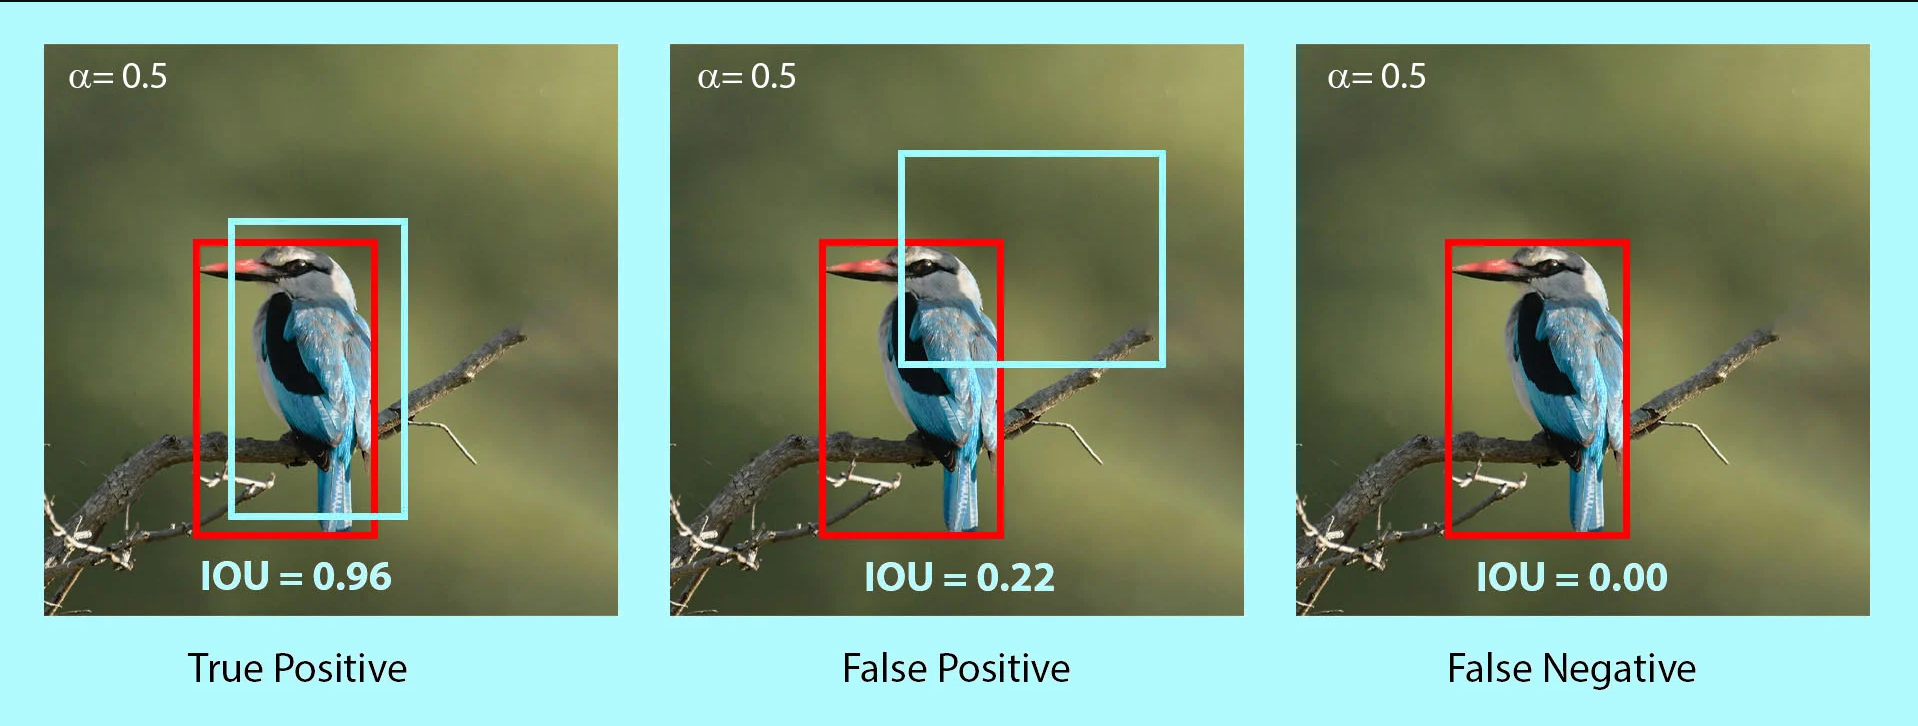
\includegraphics{figures/01-chapter1/4-birds-prediction-types-1.png}
The .50:.05:.95 means that one uses 10 IoU thresholds of \(\{0.50, 0.55, 0.60, \dots ,0.95\}\). COCO uses this as primary metric, because it rewards detectors with better localization \citep{coco_eval}.

Object detection and image segmentation are both tasks which are concerned with localizing objects of interest in an image, but in contrast to object detection image segmentation focuses on pixel-level grouping of different semantics.

Image segmentation can be splitted into various tasks including instance segmentation, panoptic segmentation, and semantic segmentation. Instance segmentation is a task that requires the identification and segmentation of individual instance in an image. Semantic segmentation is a task that requires segmenting all the pixels in the image based on their class label. Panoptic segmentation is a combination of semantic and instance segmentation. The task is to classify all the pixels belonging to a class label, but also identify what instance of class they belong to. Panoptic and instance segmentation is often done on COCO.

\hypertarget{ade20k}{%
\paragraph{ADE20k}\label{ade20k}}

Semantic segmentation can be done one ADE20K\citep{zhou2017scene}. ADE are the first three letters of the name Adela Barriuso, who single handedly annotated the entire dataset and 20K is a reference to being roughly 20,000 images in the dataset. This dataset shows a high annotation complexity, because any image in ADE20K contains at least five objects, and the maximum number of object instances per image reaches 273. To asses the performance of a model on the ADE20K dataset one uses the mean IoU. It indicates the IoU between the predicted and ground-truth pixels, averaged over all the classes.

In contrast to the object detection task, the definition of TP, FP, and FN is slightly different as it is not based on a predefined threshold. TP is now the area of intersection between Ground Truth and segmentation mask. FP is the predicted area outside the Ground Truth. FN is the number of pixels in the Ground Truth area that the model failed to predict. The calculation of IoU is the same as in object detection tasks. It's the intersection of the predicted and ground truth boxes aka. TP divided by the union of the predicted and ground truth boxes, which is essentially \(TP + FN + FP\).
A example is shown down below.

\begin{figure}
\centering
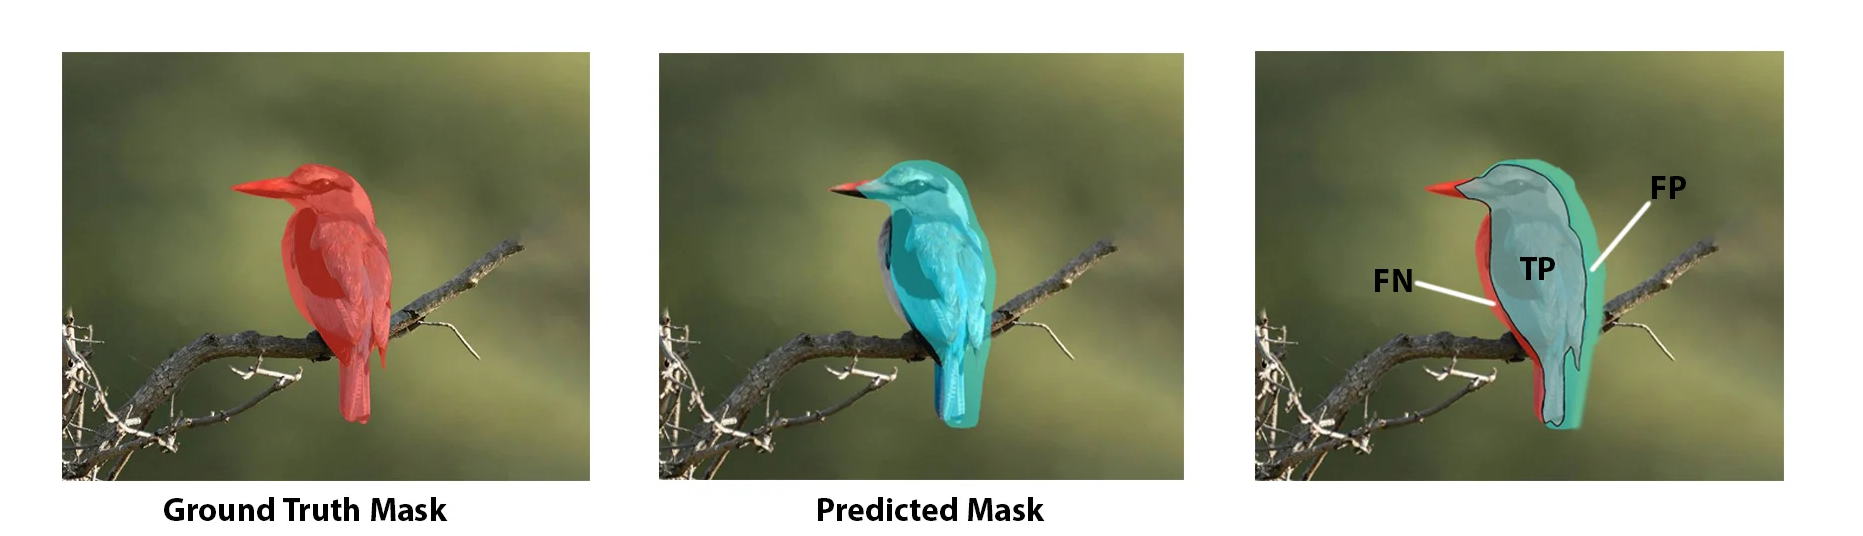
\includegraphics{figures/01-chapter1/5-segmentation-iou.png}
\caption{taken from \url{https://learnopencv.com}}
\end{figure}

\hypertarget{multi-modal-benchmarks}{%
\subsubsection{Multi-Modal Benchmarks}\label{multi-modal-benchmarks}}

Visual understanding goes well beyond object recognition or semantic segmentation. With one glance at an image, a human can effortlessly imagine the world beyond the pixels. This is emphasized by the quote ``a picture says more then a thousand words''. High-order of cognition and commonsense reasoning about the world is required to infer people's actions, goals, and mental states. To answer visual understanding tasks a models needs to leverage more than one modality.

\hypertarget{visual-commonsense-reasoning-vcr}{%
\paragraph{Visual Commonsense Reasoning (VCR)}\label{visual-commonsense-reasoning-vcr}}

Visual understanding tasks require seamless integration between recognition and cognition and this task can be formalize as Visual Commonsense Reasoning (VCR). \citet{zellers2019recognition} introduce a new dataset called VCR. It consists of 290k multiple choice QA problems derived from 110k movie scenes. The key recipe for generating non-trivial and high-quality problems at scale is Adversarial Matching. Incorrect choices are obtained via maximum-weight bipartite matching between queries and responses. This matching transforms rich annotations into multiple choice questions with minimal bias. VCR casted as a four-way multiple choice task.

The underlying scenes come from the Large Scale Movie Description Challenge and YouTube movie clips and they searched for interesting an diverse situations to ensure this they trained and applied an ``interestingnes filter''. The most interesting images were passed to Workers of Amazon Mechanical Turk. Additional context in form of video caption was given to the worker. After reading this they had to propose one to three questions about the image. For each question, they had to provide a reasonable answer and a rationale. This results is an underlying dataset with high agreement and diversity of reasoning. Almost every answer and rationale is unique. To make these cognition-level questions simple to ask, and to avoid the clunkiness of referring expressions, VCR's language integrates object tags ({[}person2{]}) and explicitly excludes referring expressions (`the woman on the right.'). These object tags are detected from Mask-RCNN. The following types of questions are in the benchmarks: 38\% Explanation (`Why is {[}person11{]} wearing sunglasses inside?'), 24\% Activity ('What are {[}person1{]} and person{[}2{]} doing?``), 13\% Temporal (''What will {[}person6{]} do after unpacking the groceries?"), 8\% Mental, 7\% Role, 5\% Scene, 5\% Hypothetical.

So in this setup, a model is provided a question, and has to pick the best answer out of four choices. Only one of the four is correct. If the model answered correctly a new question, along with the correct answer, is provided. Now the model has to justify it by picking the best rationale out of four choices. The first part is called Question Answering (\(Q\rightarrow A\)) and the second part Answer Justification (\(QA\rightarrow R\)). They combine both parts into a \(Q\rightarrow AR\) metric, in which a model only gets a question right if it answers correctly and picks the right rationale. If it gets either the answer or the rationale wrong, the entire prediction will be wrong. Models are evaluated in terms of accuracy.

The results at the release were that humans find VCR easy (over 90\% accuracy), and state-of-the-art vision models struggle (∼45\%). At the moment of writing, the best model achieves 85.5 in (\(Q\rightarrow A\)), 87.5 in (\(QA\rightarrow R\)) and 74.9 in \(Q\rightarrow AR\). So the models are closing the gap but VCR is still far from solved. An ``simpler'' approach to evaluate vision-language models is to ask questions without reasoning about an image.

\hypertarget{visual-question-answering-1.0-2.0-vqa}{%
\paragraph{Visual Question Answering 1.0 \& 2.0 (VQA)}\label{visual-question-answering-1.0-2.0-vqa}}

For this reason \citet{antol2015vqa} created an open-ended answering task and a multiple-choice task. Their dataset contains roughly 250k images, 760k questions, and 10M answers. 204k images are taken from the MS COCO dataset but also newly created created datasets are used. Three questions were collected for each image or scene. Each question was answered by ten subjects along with their confidence. The dataset contains over 760K questions with around 10M answers. ``what''-, ``how''-, ``is''- questions are mainly used in the benchmark. But they had major flaws in their creation. An model which blindly answering ``yes'' without reading the rest of the question or looking at the associated image results in a VQA accuracy of 87\% or the most common sport answer ``tennis'' was the correct answer for 41\% of the questions starting with ``What sport is'', and ``2'' is the correct answer for 39\% of the questions starting with ``How many'' \citep{antol2015vqa}.

\citet{zhang2016yin} pointed out a particular `visual priming bias' in the VQA dataset. \citet{zhang2016yin} showed that language provides a strong prior that can result in good superficial performance, without the underlying models truly understanding the visual content. \citet{zhang2016yin} collected a balanced dataset containing pairs of complementary scenes to reduce or eliminate the strong prior of the language. \citet{goyal2017making} did the same and made a second iteration of the Visual Question Answering Dataset and Challenge (VQA v2.0). \citet{goyal2017making} balanced the popular VQA dataset \citep{antol2015vqa} by collecting complementary images such that every question in balanced dataset is associated with not just a single image, but rather a pair of similar images that result in two different answers to the question. The dataset is by construction more balanced than the original VQA dataset and has approximately twice the number of image-question pairs.

\hypertarget{gqa}{%
\subsubsection{GQA}\label{gqa}}

\citet{hudson2019gqa} introduced the GQA dataset for real-world visual reasoning and compositional question answering. It consists of 113K images and 22M questions of assorted types and varying compositionality degrees, measuring performance on an array of reasoning skills such as object and attribute recognition, transitive relation tracking, spatial reasoning, logical inference and comparisons. They also proposed Consistency, Validity and Plausibility as new measures to get more insight into models' behavior and performance. Consistency measures responses consistency across different questions. To achieve a high consistency a model may require deeper understanding of the question semantics in context of the image. The validity metric checks whether a given answer is in the question scope, e.g.~responding some color to a color question. The plausibility score goes a step further, measuring whether the answer is reasonable, or makes sense, given the question (e.g.~elephant usually do not eat pizza).

They even made a comparison between GQA and VQA 2.0. They came to the conclusion that the questions of GQA are objective, unambiguous, more compositional and can be answered from the images only, potentially making this benchmark more controlled and convenient for making research progress on. Conversely, VQA questions tend to be a bit more ambiguous and subjective, at times with no clear and conclusive answer. Finally, we can see that GQA provides more questions for each image and thus covers it more thoroughly than VQA.

\hypertarget{generative-benchmarks}{%
\paragraph{Generative Benchmarks}\label{generative-benchmarks}}

Almost everybody is talking right now about generative models like DALL-E2, Imagen, Parti. It seems like every month a new one is presented. But how can we compare these models? Automatic image quality and automatic image-text alignment are two reasonable evaluation metrics. Fréchet Inception Distance (FID) can be used as primary automated metric for measuring image quality. The Frechet Inception Distance compares the distribution of generated images with the distribution of real images that were used to train the generator. A small value is wanted, as it's a distance measure. Text-image fit can be captured through automated captioning evaluation. For this an image output by the model is captioned with a model, which is able to do image captioning. The similarity of the input prompt and the generated caption is then assessed via BLEU, CIDEr, METEOR and SPICE and also human evaluation is done. Here different generative models are used with the same prompts and the human is asked to choose which output is a higher quality image and which is a better match to the input prompt. One always has to keep in mind, that the images of the generative models are always ``cherry picked''. They do not typically represent, for example, a single shot interaction in which the model directly produces such an image. To make this clear, \citet{parti} showed their way of growing the cherry tree.

\begin{figure}
\centering
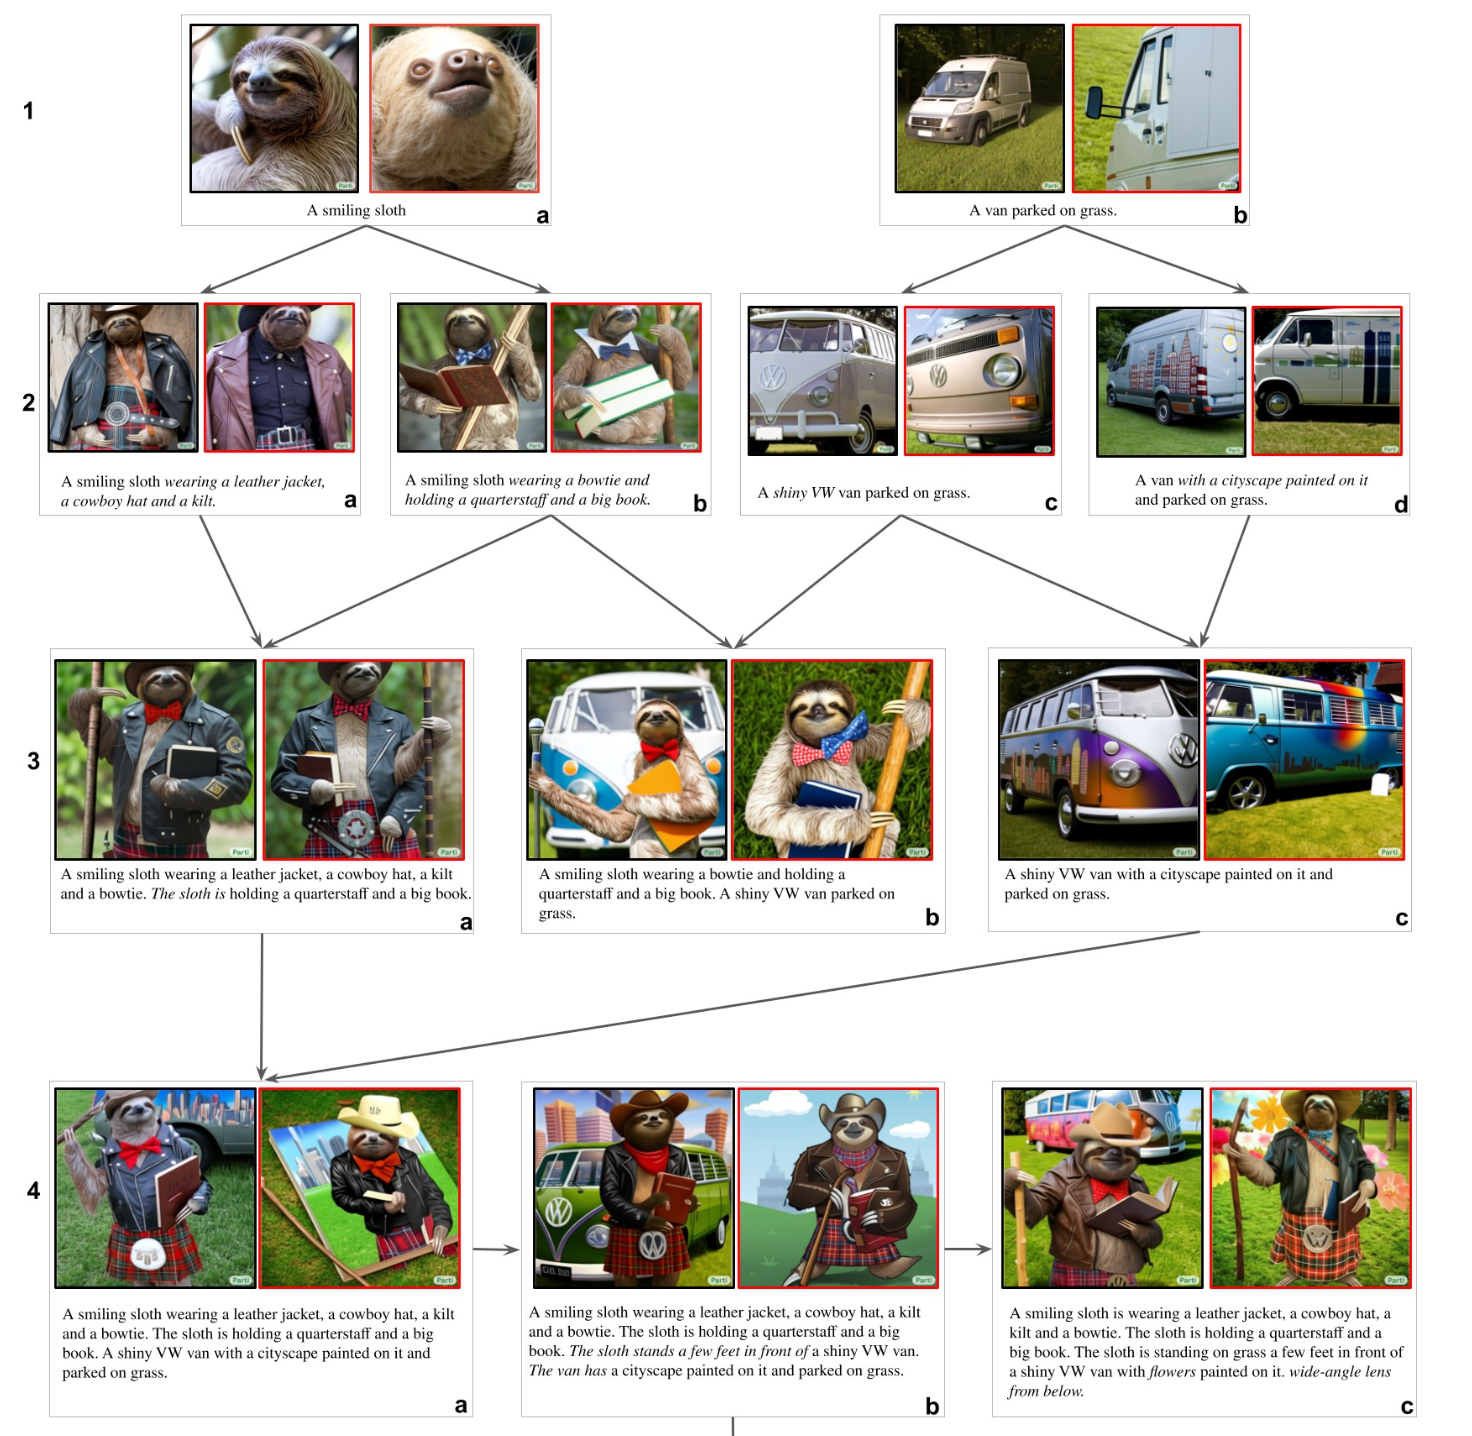
\includegraphics{figures/01-chapter1/Parti_Growing.png}
\caption{taken from Parti Paper}
\end{figure}

\hypertarget{partiprompts-drawbench-localized-narratives}{%
\paragraph{PartiPrompts, DrawBench, Localized Narratives}\label{partiprompts-drawbench-localized-narratives}}

In a sense, this is a form of model whispering as one stretches such models to their limits. Besides to that they also present PartiPrompts (P2) which is a set of over 1600 (English) prompts curated to measure model capabilities across a variety of categories and controlled dimensions of difficulty. P2 prompts can be simple, but can also be complex, such as 67-word description they created for Vincent van Gogh's The Starry Night. DrawBench is a similar dataset. Also the Localized Narratives dataset from the dataset section consists of long prompts and though it can also be used as a benchmark for generative models.

Current benchmarks give a good perspective on model performance on a wide range of V\&L tasks, but the field is only starting to assess why models perform so well and whether models learn specific capabilities that span multiple V\&L tasks.

\hypertarget{foil-it}{%
\paragraph{FOIL it!}\label{foil-it}}

\citet{shekhar2017foil} proposed an automatic method for creating a large dataset of real images with minimal language bias and some diagnostic abilities. They extended the MS-COCO dataset and created FOIL-COCO. FOIL stands for ``Find One mismatch between Image and Language caption'' and consists of images associated with incorrect captions. The captions are produced by introducing one single error (or `foil') per caption in existing, human-annotated data. So each datapoint FOIL-COCO can be described as triplet consisting of an image, original and foil caption. Their data generation process consists of four main steps:

\begin{enumerate}
\def\labelenumi{\arabic{enumi}.}
\tightlist
\item
  Generation of replacement word pairs
\item
  Splitting of replacement pairs into training and testing
\item
  Generation of foil captions
\item
  Mining the hardest foil caption for each image
\end{enumerate}

The models are evaluated on three different tasks. The first one is Correct vs.~foil classification. Given an image and a caption, the model is asked to mark whether the caption is correct or wrong. The aim is to understand whether LaVi models can spot mismatches between their coarse representations of language and visual input. The second task is Foil word detection. Given an image and a foil caption, the model has to detect the foil word. The aim is to evaluate the understanding of the system at the word level. The last task Foil word correction. Given an image, a foil caption and the foil word, the model has to detect the foil and provide its correction. The aim is to check whether the system's visual representation is fine-grained enough to be able to extract the information necessary to correct the error. Their hypothesis is that systems which, like humans, deeply integrate the language and vision modalities, should spot foil captions quite easily.

\hypertarget{valse}{%
\paragraph{VALSE}\label{valse}}

Vision And Language Structured Evaluation (VALSE) \citep{parcalabescu-etal-2022-valse} builds on the same idea. This benchmark aims to gauge the sensitivity of pre-trained V\&L models to foiled instances. They coverd a wide spectrum of basic linguistic phenomena affecting the linguistic and visual modalities: existence, plurality, counting, spatial relations, actions, and entity coreference. To generate the foils they first use strong language models to propose foil and second they use natural language inference to filter out captions that still can describe the image. To do this in an automatic fashion they use the image as an premise and the caption its entailed hypothesis. Additionally they use the captian as an premise and the foil as the hypothesis. If an NLI model predicts the foil to be neutral or a contradiction with respect to the caption, they see this as an indicator for a good foil. At last the used human annotators to validate all generated testing data. Mainly the MS-COCO dataset is used. VALSE is as a task-independent, zero-shot benchmark to assess the extent to which models learn to ground specific linguistic phenomena as a consequence of their pretraining.

\hypertarget{other-benchmarks}{%
\subsubsection{Other Benchmarks}\label{other-benchmarks}}

As we don't live in a world with unlimited resources, it's also important to keep track of how much energy is consumed to train the models and how big the carbon footprint is. \citet{strubell2019energy} investigated some NLP models and benchmarked model training and development costs in terms of dollars and estimated \(CO_2\) emissions. They came to the result that training a single BERT base model without hyperparameter tuning on GPUs requires the same energy as a trans-American flight. On average a human is responsible for 5t \(CO_2\) per year and \citet{strubell2019energy} estimated that the training procedure of a big Transformer with neural architecture search emitted 284t of \(CO_2\). Works \citep[\citet{henderson2020towards}]{lottick2019energy} have released online tools to benchmark their energy usage and initiatives such as the \href{https://sites.google.com/view/sustainlp2020/organization}{SustainNLP workshop} have since taken up the goal of prioritizing computationally efficient hardware and algorithms. These findings are just some points one should keep in mind.

In the following chapters we will see how the multimodal architectures use these datasets and also how they perform on the given benchmarks.

\hypertarget{multimodal-architectures}{%
\chapter{Multimodal architectures}\label{multimodal-architectures}}

\emph{Authors: Luyang Chu, Karol Urbanczyk, Giacomo Loss, Max Schneider, Steffen Jauch-Walser}

\emph{Supervisor: Christian Heumann}

Multimodal learning refers to the process of learning representations from different types of input modalities, such as image data, text or speech.
Due to methodological breakthroughs in the fields of Natural Language Processing (NLP) as well as Computer Vision (CV), in recent years multimodal models have gained increasing attention as they are able to strengthen predictions and better emulate the way humans learn.
This chapter focuses on discussing images and text as input data.
The remainder of the chapter is structured as follows:

The first part ``Image2Text'' discusses how transformer-based architectures improve meaningful captioning for complex images using a new large scale, richly annotated dataset COCO \citep{mccoco, cornia2020m2}.
Whether it is seeing a photograph and describing it or parsing a complex scene and describing its context, it is not a difficult task for humans.
But it is much more complex and challenging for computers.
We start with focusing on images as input modalities.
In 2014 Microsoft COCO was developed with a primary goal of advancing the state-of-the-art (SOTA) in object recognition by diving deeper into a broader question of scene understanding \citep{mccoco}.
COCO stands for Common Objects in Context.
It addresses three core problems in scene understanding: object detection (non-iconic views), segmentation, and captioning.
For tasks like machine translation and language understanding in NLP, transformer-based architecture is widely used.
However, the potential of these applications in the multi-modal context has not been fully covered.
With the help of the COCO dataset, a transformer-based architecture: Meshed-Memory Transformer for Image Captioning (\(M^2\)) will be introduced to improve both image encoding and the language generation steps \citep{cornia2020m2}.
The performance of the (\(M^2\)) Transformer and different fully-attentive models will be evaluated and compared on the COCO dataset.

Next, in ``Text2Image'', the idea of incorporating textual input in order to generate visual representations is described.
Current advancements in this field have been made possible largely due to recent breakthroughs in NLP, which first allowed for learning contextual representations of text.
Transformer-like architectures are being used to encode the input into embedding vectors, which are later helpful in guiding the process of image generation.
The chapter looks into details and discusses two SOTA model architectures by OpenAI, which both condition on text representations.
Surprisingly, none of them uses a GAN approach - a method which probably has been seen as the go-to idea for image generation over the last years.
The first model is DALL-E \citep{ramesh2021dalle}, which essentially combines Variational Encoder (VAE) with Autoregressive Transformer.
In the first step, VAE is being trained to learn downsized image representations.
Such embeddings are concatenated with text embeddings into one text-image pair input.
However, both of them use different dimensionality and vocabulary size.
In the second step, the transformer is trained on a next token prediction task given these data pairs.
Finally, at inference time, the model is able to generate images in the following way:

\begin{enumerate}
\def\labelenumi{\arabic{enumi}.}
\tightlist
\item
  Encode text input into text embedding
\item
  Use trained transformer from step 2 to generate image embedding
\item
  Use VAE from step 1 to generate image from image embedding
\end{enumerate}

The next approach to text-to-image generation is a GLIDE model \citep{nichol2021glide}.
GLIDE stands for Guided Language to Image Diffusion for Generation and Editing.
Its idea is to use Diffusion Models.
In its core, Diffusion Model is a simple idea -- random noise is being added to the image in an iterative fashion, and then model learns how to reconstruct this image.
In the case of GLIDE this learning process is conditioned on the text prompt, which is first passed through a transformer.
Both models differ in their results.
While DALL-E's resulting images might have been overwhelming back in the beginning of 2021, GLIDE is thought to significantly improve on photorealism and resolution the generated images.
Since the field has already seen further improvements following GLIDE, these new developments are also going to be mentioned in the chapter.

The third part, ``Images supporting Language Models'', deals with the integration of visual elements in pure textual language models.
Distributional semantic models such as Word2Vec and BERT assume that the meaning of a given word or sentence can be understood by looking at how (in which context) and when the word or the sentence appear in the text corpus, namely from its ``distribution'' within the text.
But this assumption has been historically questioned, because words and sentences must be grounded in other perceptual dimensions in order to understand their meaning \citep[see for example the ``symbol grounding problem'';][]{harnad1990symbol}.
For these reasons, a broad range of models has been developed with the aim to improve pure language models, leveraging on the addition of other perceptual information, such as visual ones.
This subchapter focuses in particular on the integration of visual elements (images) to support pure language models for various tasks at the word-level and sentence-level.
The starting point is always a language model, on which visual representations (extracted often with the help of large pools of images like MS COCO, see chapter ``Img2Text'' for further references) are to be ``integrated''.
But how?
There has been proposed a wide range of solutions:
On one side of the spectrum, textual elements and visual ones are learned separately and then ``combined'' together whereas on the other side, the learning of textual and visual features takes place simultaneously/jointly.

\begin{figure}

{\centering 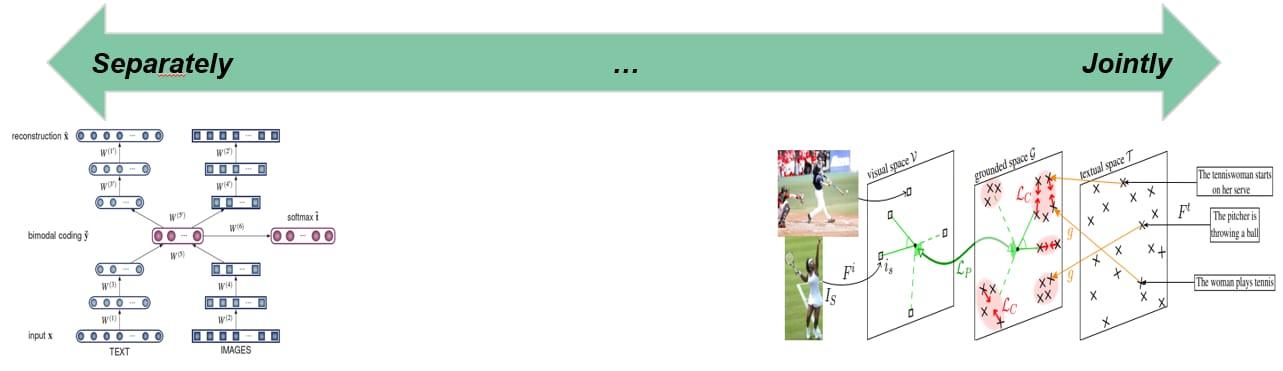
\includegraphics[width=1\linewidth]{figures/02-chapter2/Img_Ch_Intro} 

}

\caption{Left, Silberer et al., 2014: stacked autoencoders to learn higher-level embeddings from textual and visual modalities, encoded as vectors of attributes. Right, Bordes et al., 2020: textual and visual information fused in an Intermediate space denoted as “grounded space”; the “grounding objective function” is not applied directly on sentence embeddings but trained on this intermediate space, on which sentence embeddings are projected.}\label{fig:unnamed-chunk-1}
\end{figure}

For example, \citet{silberer2012grounded} implement a model where a one-to-one correspondence between textual and visual space is assumed.
Text and visual representations are passed to two separate unimodal encoders and both outputs are then fed to a bimodal autoencoder.
On the other side, \citet{bordes2020incorporating} propose a ``text objective function'' whose parameters are shared with an additional ``grounded objective function''.
The training of the latter takes place in what the authors called a ``grounded space'', which allows to avoid the one-to-one correspondence between textual and visual space.
These are just introductory examples and between these two approaches there are many shades of gray (maybe more than fifty\ldots).
These models exhibit in many instances better performance than pure language models, but they still struggle on some aspects, for example when they deal with abstract words and sentences.

Afterwards, in ``Text supporting Image Models'', approaches where natural language is used as supervision for CV models are described.
Intuitively these models should be more powerful compared to models supervised solely by manually labeled data, simply because there is much more training data available.
An important example for this is the CLIP model \citep{radford2021learning} with its new dataset WIT (WebImageText) comprising 400 million text-image pairs scraped from the internet.\\
Similar to ``Text2Image'' the recent successes in NLP have inspired new approaches in this field.
Most importantly pre-train methods, which directly learn from raw text \citep[e. g. GPT-n, Generative Pre-trained Transformer;][]{brown2020language}.
So, CLIP stands for Contrastive Language-Image Pre-training.
A transformer-like architecture is used for jointly pre-training a text encoder and an image encoder.
For this the contrastive goal to correctly predict which natural language text pertains to which image inside a certain batch, is employed.
Training this way turned out to be more efficient than to generate captions for images.\\
This leads to a flexible model, which at test time uses the learned text encoder as a ``zero-shot'' classifier on embeddings of the target dataset's classes.
The model, for example, can perform optical character recognition, geo-location and action-recognition.
Performance-wise CLIP can be competitive with task-specific supervised models, while never seeing an instance of the specific dataset before.
This suggests an important step towards closing the ``robustness gap'', where machine learning models fail to meet the expectations set by their previous performance -- especially on ImageNet test-sets -- on new datasets.

Finally, ``Text plus Images'' discusses how text and image inputs can be incorporated into a single unifying framework in order to get closer to a general self-supervised learning model.
There are two key advantages that make such a model particularly interesting.
Similar to models mentioned in previous parts, devoid of human labelling, self-supervised models don't suffer from the same capacity constraints as regular supervised learning models.
Nevertheless, while there have been notable advances in dealing with different modalities, it is often unclear to which extend a model structure generalizes across different modalities.
Rather than potentially learning modality-specific biases, a general multipurpose framework can help increase robustness while also simplifying the learner portfolio and thereby better emulating human learning processes.\\
Data2vec \citep{baevski2022data2vec} is a new multimodal self-supervised learning model which uses a single framework for either speech, NLP or computer vision.
This is in contrast to earlier models which used different algorithms for different modalities.
The core idea of data2vec, developed by MetaAI, is to predict latent representations of the full input data based on a masked view of the input in a self-distillation setup using a standard transformer architecture \citep{baevski2022data2vec}.
As a result, the main improvement is in the framework, not the underlying models themselves.
For example, the transformer architecture follows \citet{vaswani2017attention}.
Transformers have several advantages over CNNs, such as encoding the relative position of features (citation needed).
The central building block of the data2vec framework is a student-teacher structure that allows the learning process to occur without supervision.
To achieve this, inputs serve both as training data and as learning targets by being masked.
A key issue to be aware of is model collapse, i.e the model collapsing into a constant representation.
Normalization helps prevent that, as well as the domination of certain layers with high norm.
The encoding, normalization and masking strategies are modality-specific.
However, the learning objective remains the same across all modalities.
The model is trained to predict the model representation of the original unmasked training sample.
As a result of the use of self-attention in creating teacher representations, the data2vec model works with continuous and contextualized targets which are richer in information than a fixed set of targets based on local context as used in most prior work.
On top of that, working with latent representations of the network itself can be seen as a simplification of many prior modality-specific models \citep{baevski2022data2vec}.
As far as the results are concerned, data2vec is effective in all three modalities.
It sets new SOTA scores on computer vision, speech recognition as well as speech learning benchmarking sets.

\hypertarget{img2text}{%
\section{img2text}\label{img2text}}

*Author: Luyang Chu

*Supervisor: Christian Heumann

\hypertarget{microsoft-coco-common-objects-in-context}{%
\subsection{2.1.1 Microsoft COCO: Common Objects in Context}\label{microsoft-coco-common-objects-in-context}}

Understanding of visual scenes plays an important role in computer vision research (CV)
Many tasks are included in it, such as image classification, object detection, object localization and semantic scene labeling.
Through the computer vision research history, Image Datasets have played a critical role. They are not only essential for training and evaluating new algorithms, but also lead the research to new challenging directions.\citep{mccoco} In the early year, researchers developed Datasets{[}345{]} which enabled the direct comparison of hundreds of image recognition algorithms, that was the early evolution in object recognition. Recent years, ImageNet dataset {[}1{]} which contains millions of images has enabled breakthroughs in both object classification and detection research using new deep learning algorithms.
With the goal of advancing the state-of-art in object recognition especially scene understanding, a new large scale data called Microsoft COCO was published in 2014. MS COCO focuses on three core problems in scene understanding: detecting non-iconic views, detecting the semantic relationships between objects and precise localization of image objects.\citep{mccoco}
MS COCO Dataset contains 91 common object categories with a total of 328,000 images as well as 2,500,000 labeled instances. All these images could be recognized by a 4 year old child.82 categories include more than 5000 labeled The labeled instances which may support the detection of relationships between objects is much larger per image in COCO (7.7) than in ImageNet(3.0)\citep{mccoco}. In order to provide precise localization of object instances, only ``Thing'' categories like car, table, dog will be included. objects which do not have clear boundaries like sky, sea, grass, will not be included. In current object recognition research, algorithms perform well on images with iconic views. These images always contains the single object category in the center of the image. To accomplish the goal of detecting the contextual relationships between objects, more complex images with multiple objects or natural images which comes from our daily life are gathered for the Dataset.

2.Image collection and annotation 2.1 categories2.2 non-iconic2.3 annotation
COCO is a large-scale richly annotated Datatset, the progress of building consists of two phases:Data collection and image annotation.

In order to select representative object categories for Images in COCO, researchers collected several categories from different dataset like PASCAL VOC and other sources. All these object categories can be recognized by children between 4 to 8. The quality of the object categories were ensured by co-authors.Co-authors scale the categories from 1 to 5 depending on their common occurrence, practical applications and diversity from other categories \citep{mccoco}.The final number pf the list is 91, which includes all the categories from PASCAL VOC

With the help of representative object categories, COCO want to collect a dataset which a majority of these images are non-iconic. Images are roughly divided into three types:iconic-object images, iconic-scene images and non-iconic images\citep{mccoco} (Images needs to be added)
Images are collected through two strategies, firstly images from Flickr which contains photos uploaded by amateur photographer with keywords are collected. Secondly, Searching for pairwise combination of object categories like ``dog + car'' are used by researchers to gather more non-iconic images and images with rich contextual relationships.

Due to the the scale of the dataset and the high cost of the annotation process, the design of a high quality annotation pipeline with efficient cost is a difficult task.
The annotation pipeline for COCO is splitted into three primary tasks: 1. category labeling, 2.instance spotting, and 3. instance segmenting.

\begin{figure}

{\centering 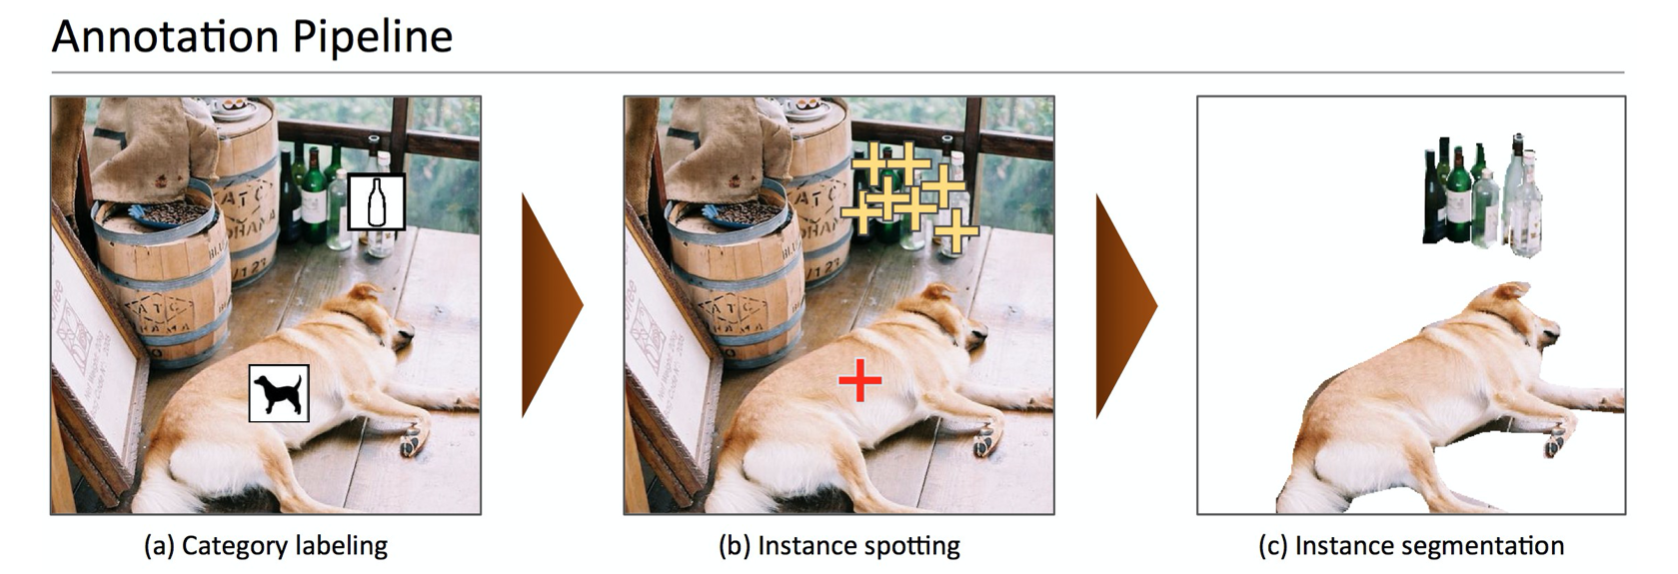
\includegraphics[width=1\linewidth]{figures/02-chapter2/2.1 annotation pipeline} 

}

\caption{Left, [@mccoco]}\label{fig:unnamed-chunk-2}
\end{figure}

As we can see in the Image(), object categories in each image will be determined in the first step. Due to the large number of Datasets and categories, they used a hierarchical approach instead of doing binary classification for each category. All the 91 categories have divided into 11 super-categories.The worker will examine the existence of a single instance for a given super-category. This hierarchical approach has helped to reduce the time for labeling. However, the first phase still took ∼20k worker hours to complete.
In the next step, all instances of the object categories in an image were labeled, at most 10 instances of a given category per image will be labeled by each worker. Each image was labeled by 8 workers for a total of ∼10k worker hours.
In the final segmenting stage, each object instance is segmented, the segmentations for other instances and the specification of the object instance by a worker in the previous stage will also shown to the worker.
( all workers are required to complete a training task for each object category. The training task required workers to segment an object instance. )
To ensure good quality an explicit verification step on each segmented instance was performed.
(high cost of time and money \ldots\ldots.)

3.datasets ---\textgreater{} further development, the pro cons
In recent years, researchers have developed several pre-trained datasets and benchmarks which helped the developemnt of Algorithms for CV.(from \ldots. simple ones?)
Each of these datasets varies significantly in size, list of labeled categories and types of images.
ImageNet containing millions of images has enabled breakthroughs in both object classification and detection research using a new class of deep learning algorithms.ImageNet was created to capture a large number of object categories, many of which are fine-grained. SUN focuses on labeling scene types and the objects that commonly occur in them. Finally, PASCAL VOC's primary application is object detection in natural images. MS COCO is designed for the detection and segmentation of objects occurring in their natural context. \citep{mccoco}
3.1.comparison with other datasets like ImageNet Pascal and SUN using the Fig from \citep{mccoco}

\begin{figure}

{\centering 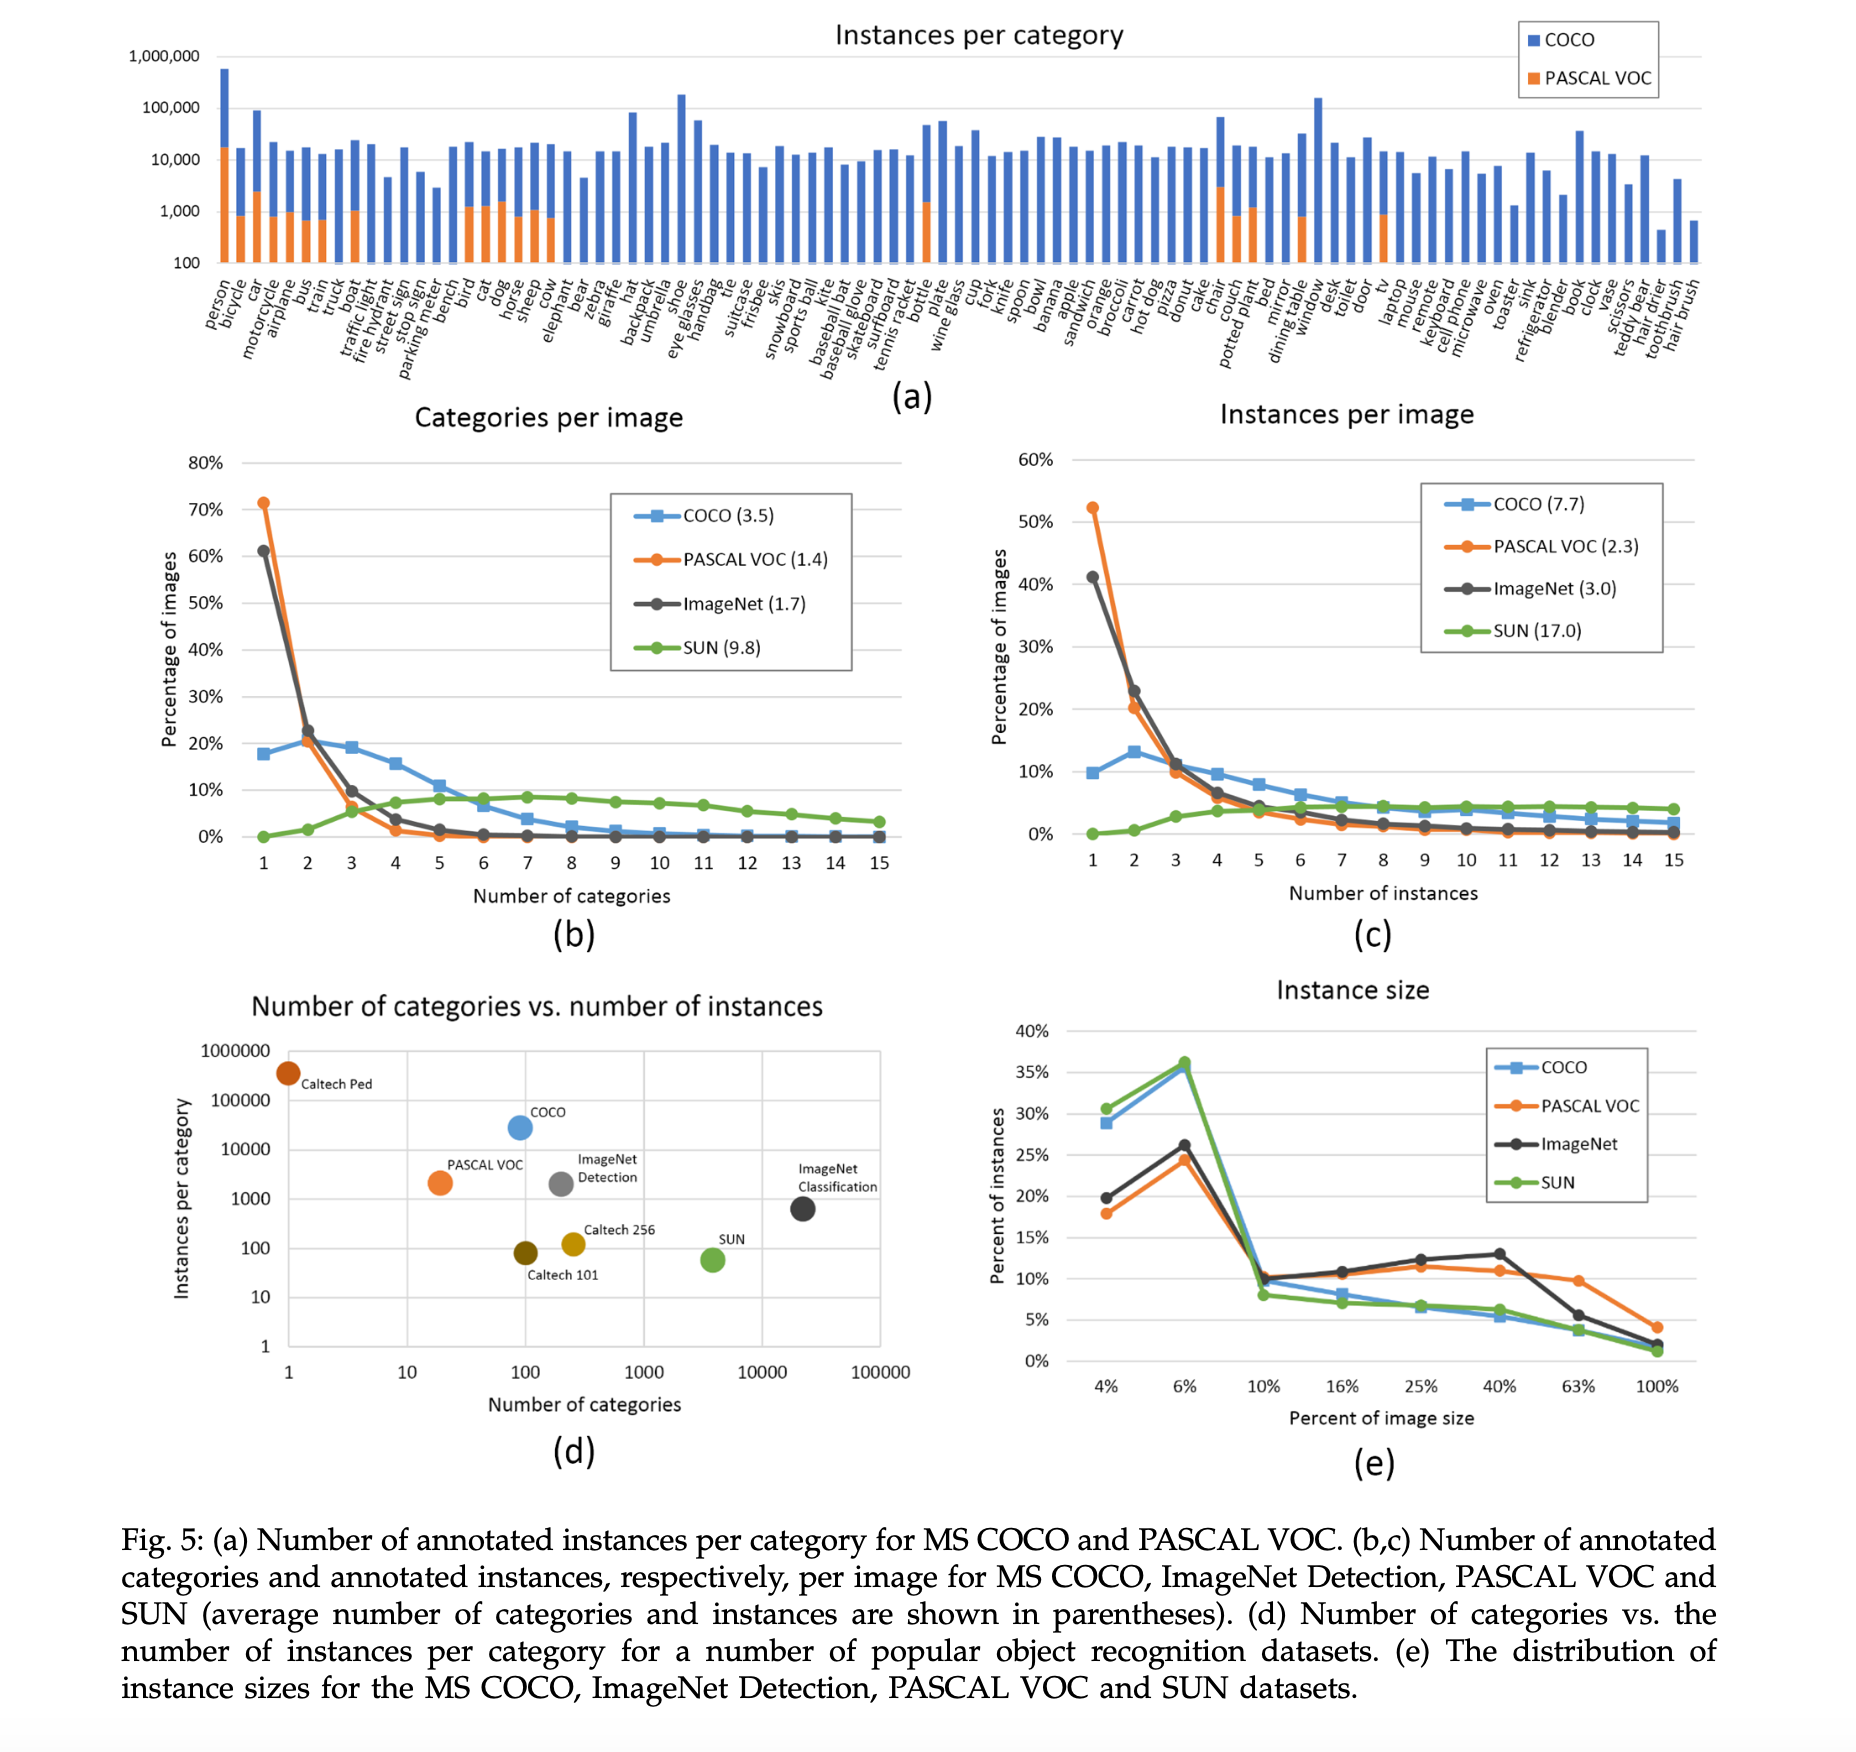
\includegraphics[width=1\linewidth]{figures/02-chapter2/2.1 coco cmparison} 

}

\caption{Left, [@mccoco]}\label{fig:unnamed-chunk-3}
\end{figure}

3.2.conclusion further development and pros cons\ldots{}
new large scale data set for detecting and segmenting objects found in everyday life
vast cost and over 70,000 worker hours
advancement of object detection and segmentation algorithms
focus non-iconic images of objects in natural environments
rich contextual information with many objects present per image.
a good benchmark for other types of labels, including scene types, attributes and full sentence written descriptions
using coco for the Meshed-Memory Transformer in 2.1.2

Questions \& pros cons
only label ``things'', but labeling ``stuff'' may also provide significant contextual information
typical vision datasets are labor intensive and costly to create
teaching only a narrow set of visual concepts;
standard vision models are good at one task and one task only, and require significant effort to adapt to a new task;
models that perform well on benchmarks have disappointingly poor performance on stress tests

\hypertarget{meshed-memory-transformer-for-image-captioning-m2}{%
\subsection{\texorpdfstring{2.1.2 Meshed-Memory Transformer for Image Captioning (\(M^2\))}{2.1.2 Meshed-Memory Transformer for Image Captioning (M\^{}2)}}\label{meshed-memory-transformer-for-image-captioning-m2}}

\begin{enumerate}
\def\labelenumi{\arabic{enumi}.}
\tightlist
\item
  what is \(m^2\) intro, the goal of it.
  Transformer-based architectures not only for language understanding.
  Exploring their applicability to multi-modal contexts like image captioning\citep{cornia2020m2}
\end{enumerate}

Image captioning: describe visual content of an image in human language.
Understand and model the relationships between visual and textual elements
Generate a sequence of output words.
\(m^2\)
A Meshed Transformer with Memory for Image Captioning
Improves both the image encoding and the language generation steps
Encoder: a multi-level representation of the relationships between image regions with a priori knowledge
Decoder: a mesh-like connectivity betwwen encoder and decoder to exploit low- and high-level features
Compare performance of the Transformer and different fully-attentive models with recurrent ones
2. \(m^2\) Transformer architecture \citep{cornia2020m2}

\begin{figure}

{\centering 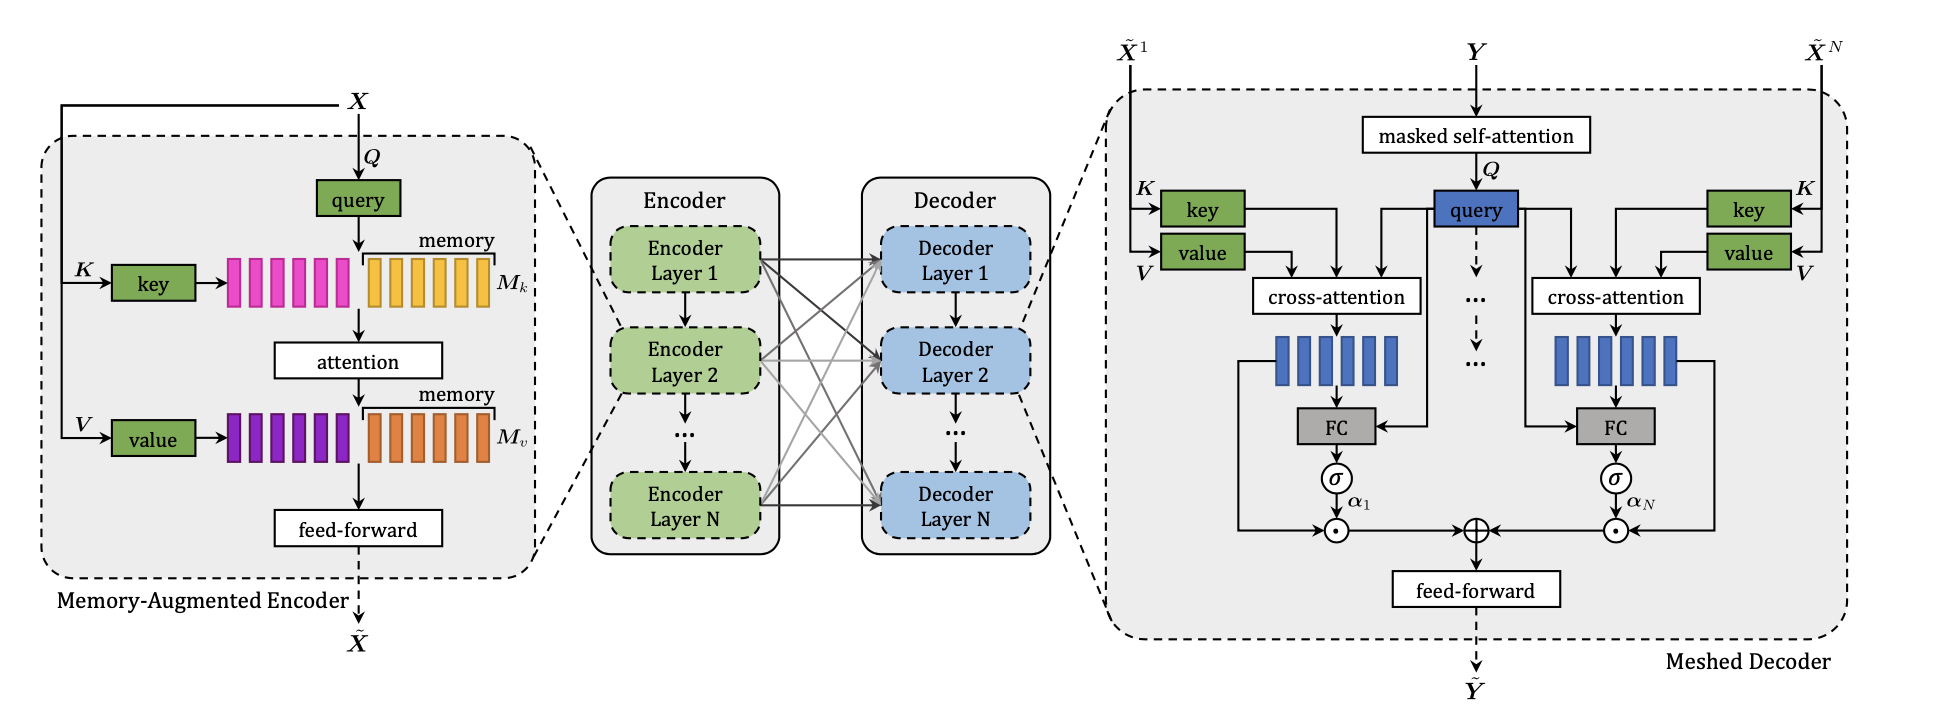
\includegraphics[width=1\linewidth]{figures/02-chapter2/2.1 m2} 

}

\caption{Left, [@mccoco]}\label{fig:unnamed-chunk-4}
\end{figure}

inspiration from the Transformer model{[}5{]}for machine translation with two new concerns
a. Image regions and their relationships encoded through multilevel encoder, take low and high level relations into account
use using persistent memory vectors to learn and encode a priori knowledge
b. exploits both low- and high-level visual relationships through the multi-layer decoder using the weights from a learnable gating mechanism fat each level
A mesh connectivity schema between encoder and decoder layers
2.1 Transformer ( should i provide short revisit for thr Transformer architecture? THE BASIC?)
All interactions between word and image-level features are modeled by using scaled dot-product attention
Attention operates on three sets of vectors, namely a set of queries Q, keys K and values V , and takes a weighted sum of value vectors according to a similarity distribution between query and key vectors.
where Q is a matrix of nq query vectors, K and V both contain nk keys and values, all with the same dimensionality, and d is a scaling factor.
\[ Attention(Q, K, V) = softmax(\frac{QK^T}{\sqrt{d}}) V, \]
2.2 Encoder with stacks of attentive layers.
Process image regions and their relationships between regions
Image region X
Attention used to get permutation invariant encoding of X through the self-attention operations
\[ S(X) = Attention(W_q X, W_k X, W_vX) \]
\$ W\_q, W\_k, W\_v\$ are learnable weights (depend solely on the pairwise similarities between linear projections of the input set X)
Output : a weighted sum of the values X
Significant limitation of self-attention: cannot model prior knowledge on relationships between image regions.
To overcome the limitation, introduce Memory-Augmented Attention by extending the keys and values with additional prior information which does not depend on image region X.
Initialize additional keys and values as plain learnable vectors which can be directly updated via SGD.
\[M_{mem}(X) = Attention(W_qX, K, V )\]
\[K = [W_kX,M_k]\]
\[V =[W_vX,M_v]\]
\(M_k\) and \(M_v\) are learnable matrices
Encoding layer: embed memory-augmented operator into a Transformer-like layer, output applied to position-wise feed-forward layer
\[ F(X)_i= U\sigma(V X_i +b)+c;\]
\(X_i\) indicates the i-th vector of the input set, and \(F(X)_i\) the i-th vector of the output. Also, \(\sigma(·)\) is the ReLU activation function, V and U are learnable weight matrices, b and c are bias terms.

Enclose the output within a residual connection and a layer norm operation.

\[ Z = AddNorm(M_{mem}(X))\]
\[ \tilde{X}=AddNorm(F(Z))\]

Full encoder: multiple encoding layers in sequence, the i-th layer uses the output set computed by layer i − 1.
higher encoding Layers can exploit and refine relationships already identified by previous layers,
N encoding layers \(\rightarrow\) multi level output \(\tilde{X} = (\tilde{X}^1 \dots \tilde{X}^n)\)

2.3 decoder with stacks of attentive layers
Conditioned on both previously generated words and region encodings
Input: Vector \(Y\) and output from all encoding layers \(\tilde{X}\) , connected through gated cross-attentions
Meshed Cross-Attention.
Perform a cross-attention with all encoding layers

\(C(·, ·)\) stands for the encoder-decoder cross-attention
\[M_{mesh}(\tilde{X}, Y) =\sum_{i = 1}^{N}\alpha_i C(\tilde{X^i}, Y) \]
C(·, ·) stands for the encoder-decoder cross-attention
\[ C(\tilde{X^i}, Y) = Attention(W_q Y, W_k \tilde{X^i}, W_v \tilde{X^i}) \]
\(\alpha_i\) is a matrix of weights same size as the cross-attention results
models single contribution of each encoding layer, and the relative importance between different layers.
\[\alpha_i = \sigma(W_i [Y,C(\tilde{X^i}, Y)]+b_i)\]
\(\sigma\) sigmoid activation function
Prediction of a word should only depend on previously predicted words
Decoder layer comprises a masked self- attention operation
Connection between queries derived from the t-th element of its input sequence Y with keys and values
Contains a position-wise feed-forward layer as well
\[Z = AddNorm(M_{mesh}(X,AddNorm(S_{mask}(Y )))\]
\[\tilde{Y} = AddNorm(F(Z)),\]
\(S_{mask}\): a masked self-attention over time
Input word vectors, and the t-th element of its output sequence make the prediction of a word at time t + 1, conditioned on \(Y≤t\). After taking a linear projection and a softmax operation, this encodes a probability over words in the dictionary.

2.4. Comparison
(not sure)detailed ? test on coco
or just simple explained

\begin{figure}

{\centering 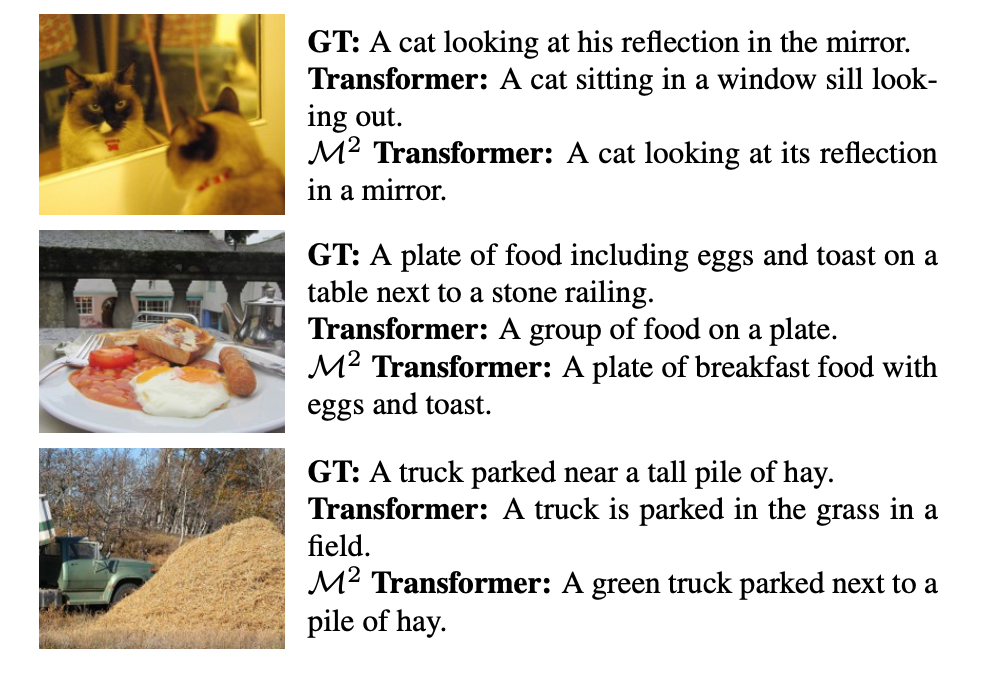
\includegraphics[width=1\linewidth]{figures/02-chapter2/2.1 m2 example} 

}

\caption{Left, [@mccoco]}\label{fig:unnamed-chunk-5}
\end{figure}

3.conclusion and bridge to next subsection

connections with other subtopics
multimodal tasks

--References( not finished)---------------------------
1.J. Deng, W. Dong, R. Socher, L.-J. Li, K. Li, and L. Fei-Fei, ``ImageNet: A Large-Scale Hierarchical Image Database,'' in CVPR, 2009.
2.M. Everingham, L. Van Gool, C. K. I. Williams, J. Winn, and A. Zis- serman, ``The PASCAL visual object classes (VOC) challenge,'' IJCV, vol.~88, no. 2, pp.~303--338, Jun.~2010
3.L. Fei-Fei, R. Fergus, and P. Perona, ``Learning generative visual models from few training examples: An incremental bayesian approach tested on 101 object categories,'' in CVPR Workshop of Generative Model Based Vision (WGMBV), 2004
4.G. Griffin, A. Holub, and P. Perona, ``Caltech-256 object category dataset,'' California Institute of Technology, Tech. Rep.~7694, 2007
5.N. Dalal and B. Triggs, ``Histograms of oriented gradients for
human detection,'' in CVPR, 20
6. Ashish Vaswani, Noam Shazeer, Niki Parmar, Jakob Uszko- reit, Llion Jones, Aidan N Gomez, Łukasz Kaiser, and Illia Polosukhin. Attention is all you need. In Advances in Neural Information Processing Systems, 2017.
7. StevenJRennie,EtienneMarcheret,YoussefMroueh,Jarret Ross, and Vaibhava Goel. Self-critical sequence training for image captioning. In Proceedings of the IEEE Conference on Computer Vision and Pattern Recognition, 2017
8..Peter Anderson, Xiaodong He, Chris Buehler, Damien Teney, Mark Johnson, Stephen Gould, and Lei Zhang. Bottom-up and top-down attention for image captioning and visual question answering. In Proceedings of the IEEE Con- ference on Computer Vision and Pattern Recognition, 2018.

\emph{Author:} Karol Urbańczyk
\#\# Text-2-image

\emph{Supervisor:} Jann Goschenhofer

\begin{itemize}
\tightlist
\item
  introduce the concept in few sentences
\item
  choice of recent break-throughs is subjective, many important ones not mentioned (GAWWN, LAFITE, Make-a-Scene, probably many others)
\end{itemize}

Intention of this chapter is to grasp how the field of text-2-image modelling has been changing over the recent years. We will start with basic concepts that has been around since 2014 and end with the state-of-the-art approaches, as of August 2022. Since the field is developing in a rapid pace, with break-through models being announced every quarter, we are aware this chapter might soon not be fully covering the field. However, we must notice that cutting edge capabilities of these models tend to come from the scale and software engineering tricks. Therefore, we believe that focusing on the core concepts should make this chapter have a universal character.

\hypertarget{seeking-objectivity}{%
\subsection{Seeking objectivity}\label{seeking-objectivity}}

\begin{itemize}
\tightlist
\item
  Objectivity in comparing generated images is very hard to grasp
\item
  However, there are some most common datasets and measures that are being used
\item
  This subchapter will quickly present them
\end{itemize}

\hypertarget{datasets-1}{%
\subsubsection{Datasets}\label{datasets-1}}

\begin{itemize}
\tightlist
\item
  COCO
\item
  CUB
\item
  Oxford 102
\end{itemize}

\hypertarget{measures}{%
\subsubsection{Measures}\label{measures}}

\begin{itemize}
\tightlist
\item
  FID (Frechet Inception Distance)
\item
  IS (Inception Score)
\item
  Human evaluations - photorealism / caption similarity
\end{itemize}

\hypertarget{generative-adversarial-networks}{%
\subsection{Generative Adversarial Networks}\label{generative-adversarial-networks}}

\begin{itemize}
\tightlist
\item
  quick intro focusing on why it is crucial to start from GANs
\end{itemize}

\hypertarget{vanilla-gan-for-image-generation}{%
\subsubsection{Vanilla GAN for Image Generation}\label{vanilla-gan-for-image-generation}}

\begin{itemize}
\tightlist
\item
  intro of GAN
\end{itemize}

\hypertarget{conditioning-on-text}{%
\subsubsection{Conditioning on Text}\label{conditioning-on-text}}

\begin{itemize}
\tightlist
\item
  how to encode the text and use it in the generation process
\item
  show some results
\end{itemize}

\hypertarget{stacking-generators}{%
\subsubsection{Stacking generators}\label{stacking-generators}}

\begin{itemize}
\tightlist
\item
  intro of StackGAN, show some results
\end{itemize}

\hypertarget{is-attention-all-you-need}{%
\subsubsection{Is attention all you need?}\label{is-attention-all-you-need}}

\begin{itemize}
\tightlist
\item
  intro of AttGAN, show some results
\end{itemize}

\hypertarget{variational-autoencoder}{%
\subsubsection{Variational Autoencoder}\label{variational-autoencoder}}

\begin{itemize}
\tightlist
\item
  Introducing the concept of VAE
\item
  How is it helpful in generating images
\end{itemize}

\hypertarget{dall-e-starting-post-gan-era}{%
\subsection{Dall-E starting post-GAN era}\label{dall-e-starting-post-gan-era}}

\begin{itemize}
\tightlist
\item
  Intro: OpenAI, dataset used, not public, etc
\item
  VQ-VAE and dVAE
\item
  Details how it's working. Combining Transformer with VQ-VAE. Training vs inference
\item
  Results and image examples
\end{itemize}

\hypertarget{glide}{%
\subsection{GLIDE}\label{glide}}

\begin{itemize}
\tightlist
\item
  Intro
\item
  Diffusion concept
\item
  details how GLIDE is working
\item
  results / scores
\item
  Limitations / strengths \& weaknesses
\end{itemize}

\hypertarget{dall-e-2}{%
\subsection{Dall-E 2}\label{dall-e-2}}

\begin{itemize}
\tightlist
\item
  Intro (mention PR move)
\item
  details how it is working
\item
  results / scores
\item
  Limitations / strengths \& weaknesses
\end{itemize}

\hypertarget{imagen}{%
\subsection{Imagen}\label{imagen}}

\begin{itemize}
\tightlist
\item
  Intro
\item
  details how it is working
\item
  results / scores
\item
  Limitations / strengths \& weaknesses
\end{itemize}

\hypertarget{parti}{%
\subsection{Parti}\label{parti}}

\begin{itemize}
\tightlist
\item
  Intro
\item
  details how it is working
\item
  results / scores
\item
  Limitations / strengths \& weaknesses
\end{itemize}

\hypertarget{open-source-community}{%
\subsection{Open-Source Community}\label{open-source-community}}

\begin{itemize}
\tightlist
\item
  Although most of the recent work comes from OpenAI and Google, there are very interesting directions taken by the open community
\item
  Mentioning the models and quickly what is happening. VQGAN+CLIP, Latent Diffusion models for sure
\item
  Maybe some links for the reader to play with?
\end{itemize}

\hypertarget{discussion}{%
\subsection{Discussion}\label{discussion}}

Mention the following points and why they matter

\begin{itemize}
\tightlist
\item
  potential business use cases
\item
  open vs closed-source (mention dall-e mini)
\item
  copyrights
\item
  biases
\end{itemize}

\hypertarget{images-supporting-language-models}{%
\section{Images supporting language models}\label{images-supporting-language-models}}

*Author: Giacomo Loss

*Supervisor: Matthias Assenmacher

\hypertarget{words-in-non-symbolic-contexts}{%
\subsection{Words In (Non-Symbolic) Contexts}\label{words-in-non-symbolic-contexts}}

Imagine you were alone in a foreign country, you could not speak the language and the only resource you had were a dictionary in the foreign language. You see a word written on a sign but you cannot understand its meaning. What could you do? One idea would be do open the dictionary and look the word up. The problem is that the word is defined by using other words in the foreign language. As a second step you would thus look these new words up and continue like that in further steps to the ``infinity and beyond'' (cit. Buzz Lightyear). But even after looking every single word in the dictionary up, you would still not be able to understand the meaning of the word written on the sign. If on that sign, next to the unknown word, something else was instead depicted, for example an image of a fork and a knife, you might speculate that the word indicates something which has to do with food, like a restaurant. And this without explicitly knowing the meaning of the word. This example is inspired by the work of Stevan Harnad, which formulated at the beginning of the 90's the so called \emph{Symbol Grounding Problem} (\citet{harnad1990symbol}). It asserts that it is not possible to understand the meaning (semantics) of a word by just looking at other words because words are essentially meaningless symbols. It is possible to understand the meaning only if the word is put in a context, a perceptual space, other than that of written language: the word must be \emph{grounded} in non-symbolic representations, like images, for example. Over the past 10 years there has been a whopping development of distributional semantic models (DSMs, henceforth), especially after the Word2vec (\citet{mikolov2013efficient}) revolution. This family of models assumes that the meaning of words and sentences can be inferred by the ``distribution'' of those words and sentences within a text corpus (the \emph{Distributional Hypothesis} formulated by \citet{harris1954distributional}). But the \emph{Symbol Grounding Problem} mentioned earlier suggests that DSMs do not resemble the way words are learned by humans, which is in multimodal perceptual contexts. For these reasons, models have been developed with the goal to integrate further modalities (like visual ones) in pure language models, assuming that grounding words and sentences in other perceptual contexts should lead to a better understanding of their semantics and, as a result, to better performance in pure language tasks.

The focus of this subchapter are models which empower pure language models with visual modalities in form of images: their goal is to obtain better semantic representations (in form of embedding vectors) of words. First, a quick recap of the main pure language models will be provided. After that, the historical evolution of the integration of images as visual modalities into pure language models will be discussed: from simple concatenation of textual and visual modalities, to the projection of visual elements in a common grounded space and more recently, the use of Transformers (see figure \ref{fig:img-hist}). Eventually, a comprehensive evaluation of the different models against benchmarks will be carried out.

Again, the focus is on how to employ visual elements to obtain embeddings able to capture the semantics of words. More concrete applications, such as those in the field of machine translation are out of scope and will be only marginally addressed at the end of the subchapter.

\begin{figure}

{\centering 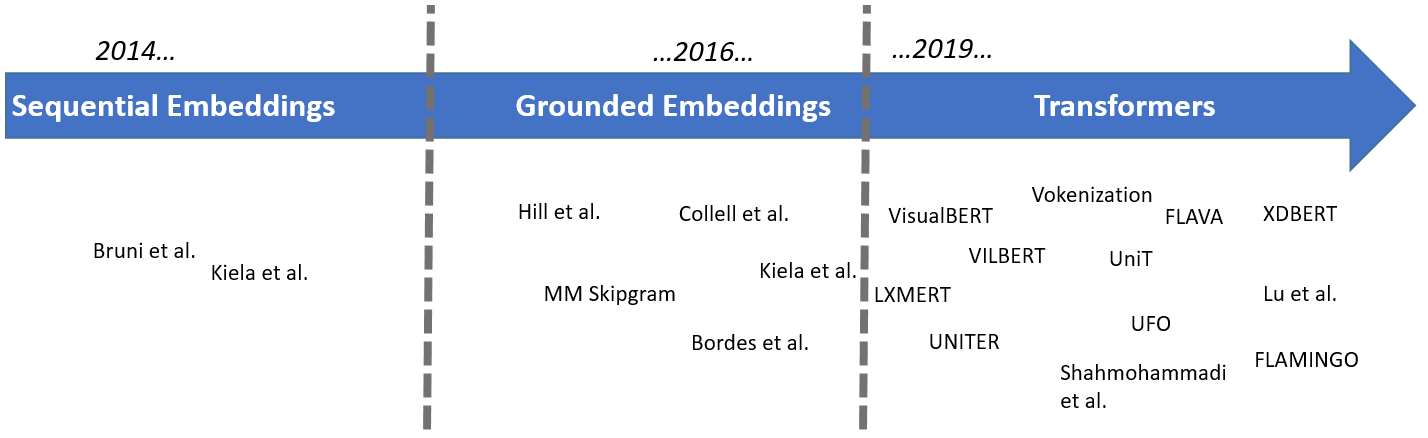
\includegraphics[width=1\linewidth]{figures/02-03-img-support-text/Img-Hist} 

}

\caption{Historical evolution of models which integrate visual information into pure language models. }\label{fig:img-hist}
\end{figure}

\hypertarget{word-embeddings-survival-kit}{%
\subsection{Word-Embeddings: Survival-Kit}\label{word-embeddings-survival-kit}}

In other parts of this books, the most important NLP-models and the latest developments in the field are extensively described. In this section, some information will be provided, which might be helpful to understand some of the aspects discussed in this subchapter. As it may have been inferred in the introduction, the starting point is always a pure language model, namely a model which employs only textual inputs in order to generate word embeddings, which are representations of words in form of numerical vectors.
The most widely used pure language models in the papers presented in this subchapter are the following three:

\begin{itemize}
\tightlist
\item
  \textbf{Skipgram} (Word2vec, \citet{mikolov2013efficient}), where given a target word, the probability of the neighboring (surrounding) words in a pre-defined window has to be maximized. Trainig takes place either through a \emph{hierarchical softmax} or through \emph{negative sampling}, which involves maximizing the probability of words which are real neighbors and minimizing that of words which are not real neighbors (the ``negative samples'')
\item
  \textbf{GloVe} (\citet{pennington2014glove}), which is based on words co-occurrence across the \emph{entire} corpus, with the goal of minimizing the difference between the dot product of the embedding vectors of two words and the logarithm of the number of co-occurrences
\item
  \textbf{BERT} (\citet{devlin2018bert}): two pre-training tasks to obtain word-embeddings:

  \begin{itemize}
  \tightlist
  \item
    Masked Language Modelling (MLM): given a sentence with {[}MASK{]}ed tokens, the goal is to predict these masked tokens
  \item
    Next Sentence Prediction (NSP): given two sentences A and B, the goal is to predict if B follows from A
  \end{itemize}
\end{itemize}

Two additional remarks to conclude this section. First, Skipgram and GloVe generate embeddings which are \emph{``context-free''}: they do not take into account the context in which words occur. On the contrary, BERT is designed to represent words given the context (sentence) in which they occur: we can thus have different embeddings for the same word, depending on the context.
Second, the inputs of these models are \emph{tokens}: with the help of a \emph{tokenizer}, which can be different for different models, the text is split in ``chunks'', called \emph{tokens} (and they are not necessarily single words).

\hypertarget{the-beginning-sequential-multimodal-embeddings}{%
\subsection{The Beginning: Sequential Multimodal Embeddings}\label{the-beginning-sequential-multimodal-embeddings}}

Supposing we add linguistic and visual feature representations related to a particular word, how could we fuse them? One intuitive idea would be to \emph{concatenate} the textual and visual modalities. Let \(V_{text}\) be the textual (vectorial) representation of a word and let \(V_{img}\) be its visual (vectorial) representation, a fused representation \(F\) of a certain word \(w\) might take the following simplified form:

\[F=\gamma(V_{text})\bigoplus(1-\gamma)V_{img}\]

where \(\gamma\) is a tuning parameter which controls the relative contribution of both modalities to the final fused representation. \citet{bruni2014multimodal} propose a model where the meaning of a target word is represented in the form of a semantic vector and all vectors are collected in a \emph{text-based semantic matrix}; textual embeddings are computed based on (transformed) co-occurrence counts of words in a pre-defined window. The starting point to obtain an image-based representation of certain target word is a dataset of labeled images. For each image associated to the target word (which means that the target word is to be found in the image's caption), low-level features called ``local descriptors'' - which incorporate geometric information of specific areas of a certain picture - are extracted and then these descriptors are assigned to clusters (\emph{bags}) of ``visual words''\footnote{See for example \citet{bosch2007image} for more details on this technique, called ``bag-of-visual-words''.}. Afterwards, for each target word, visual word occurrences are summed up together to obtain the occurrence counts related to the target word. These image-based semantic vectors are then transformed and collected in an \emph{image-based semantic matrix}. The two matrices are then concatenated and projected into a common latent multimodal space with a singular value decomposition. Thanks to this process a \emph{textual \textbf{mixed} matrix} and a \emph{visual \textbf{mixed} matrix} are extracted and then combined together according to different fusion strategies to build the multimodal embeddings. In this first, relatively cumbersome (historically motivated) example, the vector representation of an image is obtained with non-trivial features engineering.

In recent years, the use of neural networks has made an ``automatic feature selection'' possible. This is what for example \citet{kiela2014learning} propose, extracting visual features from the first seven layers of a convolutional neural network (proposed by \citet{krizhevsky2012imagenet}) trained on 1.6 million images from the ImageNet database (\citet{deng2009imagenet}), which produces scores for 1,512 object categories. The linguistic part of the model relies on the Skipgram model by \citet{mikolov2013efficient} and consists of 100-dimensional vector representations. The multimodal representation is again obtained by concatenation of both modalities.

\begin{figure}

{\centering 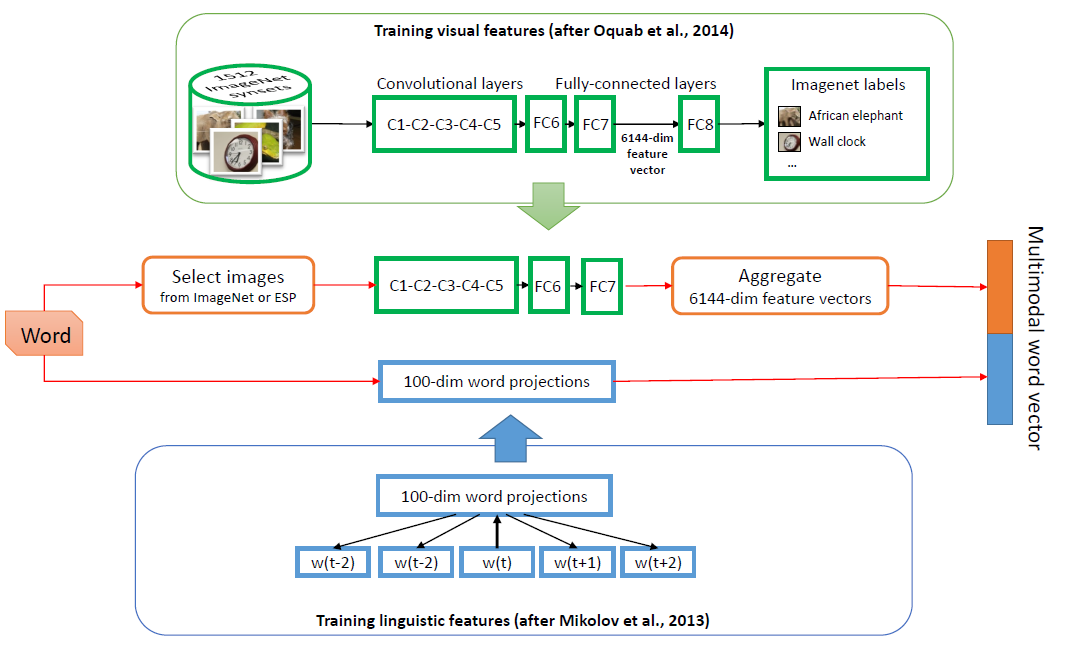
\includegraphics[width=1\linewidth]{figures/02-03-img-support-text/img-kiela2014-01} 

}

\caption{From @kiela2014learning. Textual and visual features vectors are concatenated.}\label{fig:img-kiela2014-01}
\end{figure}

Another notable example of concatenation/sequential combination of textual and visual modalities is the work of \citet{silberer2014learning}: textual and visual modalities are represented by separate vectors of textual and visual attributes. During training, these textual and visual inputs vectors are separately fed to denoising (unimodal) autoencoders, the training objective of which is the reconstruction of a certain corrupted input - e.g.~through masking noise - from a latent representation. Their outputs are then jointly fed to a bimodal autoencoder to be mapped to a multimodal space, on which a softmax layer (classification layer) is added, which allows the architecture to be fine-tuned for different tasks.

\hypertarget{the-grounded-space}{%
\subsection{The Grounded Space}\label{the-grounded-space}}

The aforementioned models assume implicitly a one-to-one correspondence between text and images: a visual representation is extracted only from words which are associated to a concrete image. This is a limitation, for two partially overlapping reasons. One one hand, how can we depict words for which no image is available in our training set? Is it possible to \emph{imagine} visual representations purely from linguistic ones? On the other hand, could we hypothetically find a visual representation for each word? This might be true for concrete words but when it comes to abstract ones, it is not always possible to find suitable visual representations or, said in other terms, many words are not visually grounded. For this reasons, researches have addressed the question: could we map textual and visual elements to a grounded space and design models able to generalize images and words beyond those in the training set? Well, the answer is yes!

\citet{lazaridou2015combining} propose a multimodal Skip-gram architecture where the objective function of a Skip-gram is ``augmented'' with an additional visual objective: \[\frac{1}{T}\sum_{t=1}^{T}\left(\mathcal{L}_{ling}(w_{t})+\mathcal{L}_{vision}(w_{t})\right)\]

where \(\mathcal{L}_{ling}\) is the Skip-gram loss function and \(\mathcal{L}_{vision}\) is the additional visual loss for the target word \(w_{t}\). In particular, \(\mathcal{L}_{vision}\) has the form of a hinge loss, the goal of which is to make the (vectorial) linguistic representation of a certain word more similar to its visual representation:

\[\mathcal{L}_{vision}(w_{t})=-\sum_{w^{'}\sim P_{n}(w)}\left(max(0,\gamma-cos(z_{w_{t}},v_{w_{t}})+cos(z_{w_{t}},v_{w^{'}})\right)\]

where \(v_{w^{'}}\) is a visual representation of a randomly chosen word \(w^{'}\) (drawn from a probability distribution \(P_{n}(w)\)) used as negative sample, \(v_{w_{t}}\) is the corresponding visual vector and \(z_{w_{t}}\) is the target multimodal word representation which has to be learned by the model. It is nothing more than a linear transformation of a word representation \(u_{w_{t}}\): \(z_{w_{t}}=M^{u\rightarrow v}u_{w_{t}}\) and \(M^{u\rightarrow v}\) is a cross-modal mapping matrix from linguistic inputs to a visual representation. It is important to remark that during training, for words which do not have associated images, \(\mathcal{L}_{vision}\) gets set to zero. When this cross-modal mapping matrix is estimated, it is then possible to find a visual representation for new words, which do not have a related image in the training set: the model allows to \emph{imagine} new words. This is what is meant with grounded space: a perceptual (visual, in this case) space where a word is \emph{grounded}, put in context.

\begin{figure}

{\centering 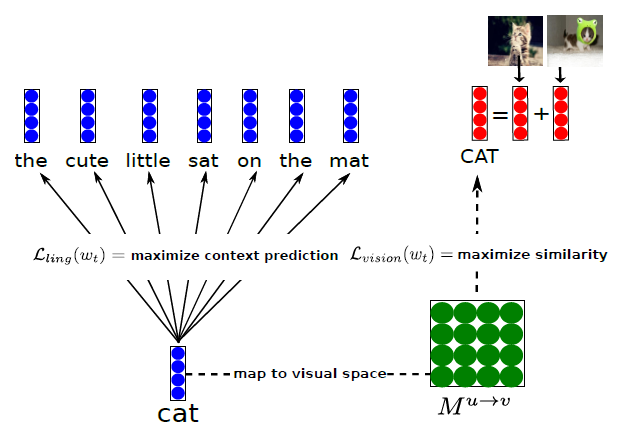
\includegraphics[width=0.8\linewidth]{figures/02-03-img-support-text/img-lazaridou2015combining01} 

}

\caption{From @lazaridou2015combining. The linguistic embedding of the word 'cat' is mapped to a visual space, such that the similarity of vector representations of words and associated images is maximized.}\label{fig:img-lazaridou2015-01}
\end{figure}

Similar instances of a cross-modal mapping can be found for example in \citet{kottur2016visual} (a multimodal extension of the CBOW model specification of word2vec) and in \citet{collell2017imagined}, where visual features are obtained from the forward pass of a CNN, pre-trained on ImageNet (\citet{deng2009imagenet}) and a mapping function from the textual space to the visual space is obtained as a result of the training process. Also in this case it is possible to generate a visual representation from the embedding of a certain word, not necessarily present in the training set. In particular, they propose two specifications of the mapping function: a simple linear mapping and neural network with a single hidden layer. Last but not least, \citet{hill2014learning} recognize that concrete nouns are more likely to have a visual representation. For this reason, they map a set of concrete words (CSLB, \citet{devereux2014centre}) to ``bags of perceptual/visual features'' and every time one of these words is encountered during training, the Skip-gram model they are using stops training on that sentence and instead continues the training on a newly created ``pseudo-sentence'', which takes into consideration the aforementioned bag of perceptual features. This list is unfortunately not exhaustive and there are other models with similar ideas, for example \citet{ailem2018probabilistic} or \citet{kiros2018illustrative}.

The aforementioned papers and related models focus on the modeling of semantics of words. Nonetheless, there are models designed to address tasks at sentence-level, such as sentiment analysis or sentence entailment. \citet{kiela2017learning} employ a bidirectional Long Short-Term Memory (LSTM, \citet{hochreiter1997long}) architecture to model sentence representations, in order to gain information from the text in both directions. The goal is again to encode a sentence and ground it in an image. Textual embeddings are obtained with GloVe (\citet{pennington2014glove}) and they are then projected on a grounded space with a linear mapping. This grounded word vector serves as input for the bidirectional LSTM, which is trained together with the linear mapping. Their model is versatile and depending on the loss function specification, it can not only propose alternative captions to an image (which is a way to frame sentence equivalence tasks) but also predict captions from images or perform both tasks at the same time. This last point highlights an important characteristic of many of the models discussed in this subchapter: even though the focus is on the empowerment of pure language models with the addition of visual elements, some of the models discussed here can be used for purposes other than pure language tasks. The control over which task is performed is usually exercised by either specifying different loss functions (as in the last model described) or setting properly certain hyperparameters (such as in the previously described model by \citet{silberer2014learning}).\\

\hypertarget{the-transformers-era}{%
\subsection{The Transformers Era}\label{the-transformers-era}}

A turning point for the field of NLP was \citet{vaswani2017attention}'s paper ``Attention is all you need'', where the authors proposed for two machine translation tasks a novel architecture, the Transformer (not to be confused with the giant robots from the Michael Bay's blockbuster movies!), which leverages only the attention mechanism. Even though an exhaustive description of the Transformer architecture is beyond the scope of this subchapter, it is worth mentioning why they became so popular over the past four years in the field of NLP (among others), in comparison to Recurrent Neural Networks (RNNs) and Long Short-Term Memory networks (LSTMs).

Well, the three main properties of Transformers are the following:

\begin{itemize}
\tightlist
\item
  Self-Attention
\item
  Parallel input processing
\item
  Positional embeddings\footnote{It may be argued that this point is a necessity to be able to work on sequences rather than a strength.}
\end{itemize}

When feeding for example a textual sentence to a RNN, the network deals with one word after the other in a sequential fashion and one of the known issues is the fact that information contained in earlier parts of the sequence tend to ``fade away'' as the sentence is analyzed further: newer inputs carry a larger influence on the outputs at a given step. LSTMs try to mitigate this problem by introducing a component called ``gate'', which regulates the information flow, namely which information from the past inputs need to be ``remembered'' by the model. The goal is to capture long-term dependencies among different parts of the sentence fed into the model.\\
On the contrary, thanks to the Self-Attention mechanism, at each step Transformers can access previous steps, thus limiting to a minimum the loss of information. Moreover, inputs are processed not sequentially but all at the same time, thus allowing to capture dependencies by looking at the sentence \emph{as a whole} and this could make a fundamental difference in many downstream applications: for example in the German language, in dependent clauses (``Nebensaetze''), the verb comes at the end of the phrase but it determines the verbal case of the nouns that come \emph{before} the verb. Thus Transformer could potentially capture the dependencies between the verb coming at the end of the sentence and the words at the beginning. Lastly, Transformers encode for every input information on its position within a sentence, since it is often the case, that the importance and meaning of a certain word varies depending on its position within a sentence. These were the Transformers, in a nutshell.

But Transformers did not only bring a change of paradigm in terms of architectures. First, while for models in the pre-Transformers era described before, the focus was on the ability of word embeddings to capture similarity among words, now the focus has shifted more on downstream tasks (more on this later in the evaluation section), encompassing not only pure linguistic ones but also tasks with visual components, such as for example, visual question answering. It is now more difficult (but not impossible) to draw a line between models where ``images support pure language models'' (the object of this subchapter) and models which could be actually categorized as ``vision and language'' models but they can be employed also to solve pure linguistic tasks. This issue brings another peculiarity of many Transformers-base models, namely their ``universal vocation'': without loss of generality we could say that the idea is now to design powerful (multimodal) pre-training (mostly \emph{self-supervised}) tasks capable of generating task-agnostic representations, whose encoded knowledge can be efficaciously transferred to diverse downstream tasks, limiting the amount of labeled data necessary to fine-tune the models (this is the so-called \emph{few-shot learning}).

Let's briefly discuss two examples, Flava (\citet{singh2022flava}) and UniT (\citet{hu2021unit}). Flava has two separate encoders for images and text and a multimodal encoder, all based on the Vision Transformer (\citet{dosovitskiy2020image}). Unimodal pre-training consists of masked image modeling (where a set of image patches are to be reconstructed from other unmasked image patches) and masked language modeling. Multimodal pre-training tasks consist instead of a global contrastive loss (maximization of cosine similarities between paired images and text), a masked multimodal modeling (where image patches and text tokens are masked) and an image-text matching task. The model is pre-trained jointly on unimodal and multimodal datasets and then evaluated (fine-tuned) on 22 vision tasks, 8 pure linguistic tasks and 5 vision and language tasks.\\
UniT has an image encoder and a text encoder, a multimodal domain-agnostic decoder and task-specific heads. There is no pre-training on multimodal data and the model is trained end-to-end on 7 tasks (vision, language and vision an language) and 8 datasets, with the idea that solving different tasks across domains in a jointly fashion should prevent general knowledge from being lost due to fine-tuning over particular downstream tasks.

These two examples clearly show what it is meant by ``universal vocation'' of many modern Transformer-based models. But there are still models specifically designed to solve pure language tasks and in the following pages, two of them will be described.

\hypertarget{vokenization}{%
\subsubsection{Vokenization}\label{vokenization}}

It is often difficult for a child to describe the meaning of a certain word. A child might not be able to describe what a lion is but if he is given pictures of different animals he might be very well able to point at the picture of a lion. \emph{Visual pointing} could thus act as a form of supervision to natural language. Is it possible to build within a pure language model a form of visual supervision, which mimics the visual pointing often adopted by children? This is exactly the problem that \citet{tan2020vokenization} try to address: how to associate to each textual representation (token) a visual representation (Voken).

Let's suppose we had a dataset of word(token)-image pairs. We could integrate in the pre-training framework of pure language models the following \emph{Voken-Classification} task:

\[\mathcal{L}_{VOKEN-CLS}(s)=-\sum_{i=1}^{l}log\ p_{i}(v(w_{i};s)|s) \]
\[\textbf{h}_{1}, \textbf{h}_{2},...,\textbf{h}_{l}=languagemodel(w_{1},w_{2},...,w_{l}) \]
\[p_{i}(v|s)=softmax_{v}\{W\textbf{h}_{i}+b\}\]
where \(\{h_i\}\) is the feature representation of each token in a sentence \(s=\{w_i\}\) extracted from a language model (such as BERT) and the vokens originate from a \textbf{finite} set of images \(X\). Each \(h_i\) is then transformed into a probability distribution through a softmax layer, with the voken-classification loss defined as the negative log-likelihood of all related vokens.\\
The model architecture would then be:

\begin{figure}

{\centering 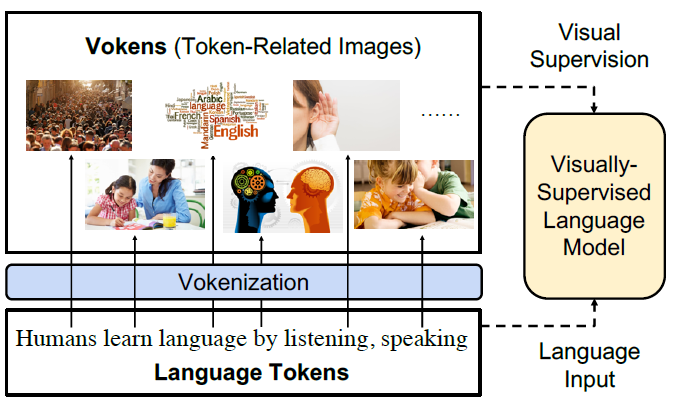
\includegraphics[width=0.7\linewidth]{figures/02-03-img-support-text/img-tan2020-04} 

}

\caption{From @tan2020vokenization. Visually supervised the language model with token-related images, called Vokens.}\label{fig:img-tan2020-04}
\end{figure}

Everything sounds fantastic! There is only one small pitfall: a set of \(X\) of images for all tokens does not exist! Could we find a proxy for such a set? One might consider image-captioning datasets such as MS COCO (\citet{lin2014microsoft}). But also this suboptimal solution is problematic.

\begin{figure}

{\centering 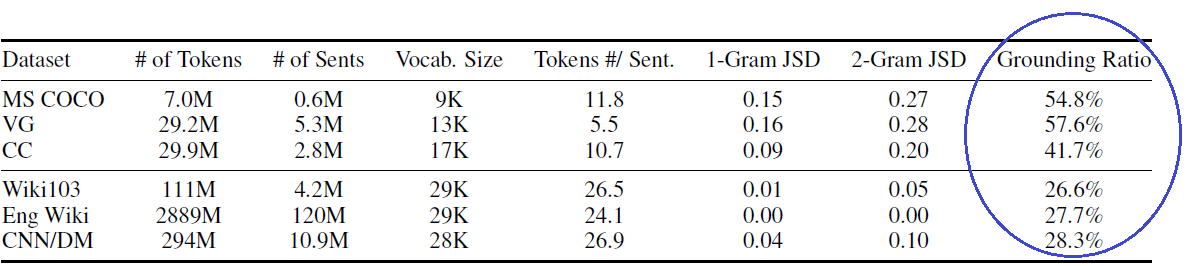
\includegraphics[width=1\linewidth]{figures/02-03-img-support-text/img-tan2020-01} 

}

\caption{From @tan2020vokenization. Statistics of image-captioning dataset and other natural language corpora. VG, CC, Eng Wiki, and CNN/DM denote Visual Genome, Conceptual Captions, English Wikipedia, and CNN/Daily Mail, respectively. JSD represents Jensen–Shannon divergence to the English Wikipedia corpus.}\label{fig:img-tan2020-01}
\end{figure}

The \emph{Grounding Ratio} is defined as the proportion of tokens in a dataset which are related to a specific visual representation (i.e.~the tokens are \emph{visually grounded}), such as ``dog'', ``table'' and the like. In figure \ref{fig:img-tan2020-01} it is striking that only around one third of tokens contained in pure language corpora such Wiki103, English Wikipedia and CNN/DM are visually grounded in image captioning datasets\footnote{From an operative point of view, the authors consider a token type ``visually grounded'' if it has more than 100 occurrences in MS COCO}. It is not possible to rely (only) on image captioning datasets to build the Voken-Classification task. But the fact that a word/token does not have a visual representation in one of these datasets, it does not mean that it is not possible to visually represent the word/token. Would it be possible to associate images to words/tokens not directly visually grounded? Well, the answer is yes!

\begin{figure}

{\centering 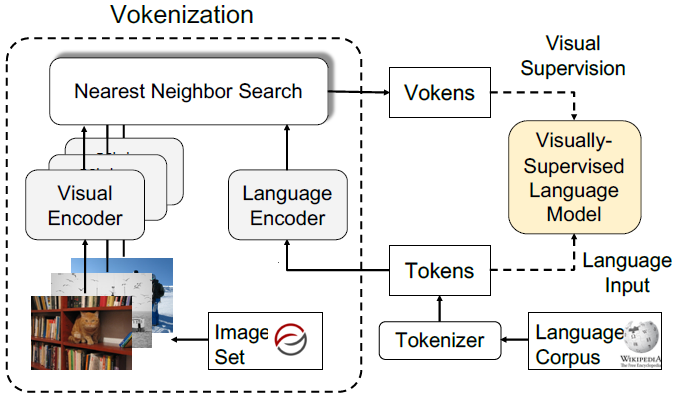
\includegraphics[width=0.8\linewidth]{figures/02-03-img-support-text/img-tan2020-05} 

}

\caption{From @tan2020vokenization. The Vokenization process. A contextualized image (visual token, Voken) is retrieved for every token in a sentence and with this visual token, visual supervision is performed.}\label{fig:img-tan2020-05}
\end{figure}

The \textbf{Vokenization} is a process to \emph{assign} every token \(w_i\) contained in a sentence \(s\) to a visual representation (called \emph{voken}) originating not from a generative model but rather from a finite set of images \(X=\{x_1,...,x_n\}\). The voken \(v(w_i;s)\) is the image from \(X\) which maximizes the following \emph{Relevance Score Function}:
\[v(w_i;s)=arg\ max_{x\in X}r_{\theta^{*}}(w_i,x,s)\]
This function takes into account not only the token \(w_i\) itself, but also the context (the sentence) and it is parametrized by \(\theta\) with \(\theta^{*}\) being the optimal value (which has to be estimated).

\hypertarget{the-relevance-score-function-model-training-inference}{%
\paragraph{The Relevance Score Function: Model, Training, Inference}\label{the-relevance-score-function-model-training-inference}}

The Relevance Score Function is defined as the inner product of the language feature representation \(f_{\theta}(w_i,s)\) and the visual feature representation \(g_{\theta}(x)\):
\[f_{\theta}(w_i,s)^Tg_{\theta}(x)\]
Supposing \(h_1,...,h_l\) and \(e\) are the embeddings originating from pre-trained language and visual encoders respectively (in the paper the authors use BERT and ResNeXt), the language and visual representations are obtained first by applying multi-layer perceptrons \(w\_mlp_{\theta}\) and \(x\_mlp_{\theta}\) to downproject the embeddings from the pre-trained models to a common vector space and secondly they are normalized (with L2-Norm):

\[ \textbf{f}_{\theta}(w_{i};s)= \frac{w{\_}mlp_{\theta}(\textbf{h}_{i})}{||w{\_}mlp_{\theta}(\textbf{h}_{i})||} \]
\[ \textbf{g}_{\theta}(x)= \frac{x{\_}mlp_{\theta}(\textbf{e})}{||x{\_}mlp_{\theta}(\textbf{e})||} \]
With respect to the training of the model, to estimate the optimal value for the parameter \(\theta\), image-captioning datasets, which are collections of sentence-image pairs, are employed. Operationally, for every sentence \(s_k\) associated to image \(x_k\) in the image-captioning dataset, each token \(w_i\) in \(s\) is associated to \(x_k\) and the \emph{hinge loss} is used to estimate the optimal value of \(\theta^*\):

\[ \mathcal{L}_{\theta}(s,x,x')=\sum_{i=1}^{l}max(0,M-r_{\theta}(w_{i},x,s)+r_{\theta}(w_{i},x',s))\]

The goal is to maximize the Relevance Score Function between aligned token-image pairs \((w_i,x;s)\) and to minimize the score for unaligned pairs \((w_i,x^{'};s)\) by at least a margin \(M\), with \(x^{'}\) being a randomly sampled image from the image captioning dataset \textbf{not} associated to sentence \(s\).

Once we have the language feature representation \(f_{\theta}(w_i,s)\) for each token in our language corpus and the optimal estimate of \(\theta\), how is it possible to find the image \(x\) encoded with the visual feature representation \(g_{\theta}(x)\), which maximizes the Relevance Score Function? As said earlier, the function is expressed as the inner product of the textual and visual representations and since the feature vectors have euclidean norm equal to 1, the inner product maximization problem is equivalent to a nearest neighbor search problem. It is just sufficient to find the vector \(g_{\theta}(x)\) which is the nearest neighbor of \(f_{\theta}(w_i,s)\)\footnote{The proof is straightforward. Let \(X\in \mathbb{R}^l\) and have euclidean norm equal to 1, which means \(||X||_{2}=1\). In the nearest neighbor search we need to find the vector \(Y\in \mathbb{R}^l\), also with norm equal to 1, which has minimal euclidean distance with \(X\). This is the quantity to be minimized:
  \begin{align*}
  d(X,Y) &=\sqrt{\sum_{i=1}^{l}{(x_i-y_i)^2}}
    \\&\stackrel{squared}{=} \sum_{i=1}^{l}{x_i^2}+\sum_{i=1}^{l}{y_i^2}-2\sum_{i=1}^{l}{x_iy_i}
    \\&\stackrel{}{=}||X||_{2}^2+||Y||_2^2-2X^TY
    \\&\stackrel{Norm-1}{=}1+1-2X^TY
    \\&\stackrel{}{=}2(1-X^TY)
  \end{align*}
  And through these simple algebraic manipulations, it is possible to see that minimizing the euclidean distance between \(X\) and \(Y\) is equivalent to maximize \(X^TY\), which is the inner product. This proves the equivalence between inner product maximization and nearest neighbor search.}.

With this process, it is thus possible to assign a visual representation, a voken, to any word/token in a language corpus, pooling from a finite set of images. The problem of the low Grounding Ratio outlined above is solved and the Voken-Classification task could be integrated in the pre-training framework of any pure language model. Moreover, the authors propose a method called \emph{Revokenization}, which allows to transfer vokens generated using a particular tokenizer to frameworks which employ other tokenizers.

\hypertarget{one-step-further-the-power-of-imagination}{%
\subsubsection{One Step Further: The Power Of Imagination}\label{one-step-further-the-power-of-imagination}}

Wikipedia defines \emph{imagination} as ``the production or simulation of novel objects, sensations, and ideas in the mind without any immediate input of the senses''. Indeed, humans do not only associate words with real images, but also leverage the ability to \emph{imagine} words/concepts: imagination can help the human brain solve problems with limited supervision or sample points by empowering its generalization capabilities. Until now we discussed language models supported by visual information in form of \emph{real} images (e.g.~those retrieved from image-captioning datasets). But with the recent advancements in the field of generative models for images, it is for sure worth investigating if these generative models can help pure language models to produce better representations of words. In particular, the framework proposed by \citet{lu2022imagination}, \textbf{iACE (Imagination-Augmented Cross-Modal Encoder)} will now be discussed: the idea is simply to use a generative model to obtain a visual representation of a textual input and then use these imagined representations as ``imagination supervision'' to pure language models.

\begin{figure}

{\centering 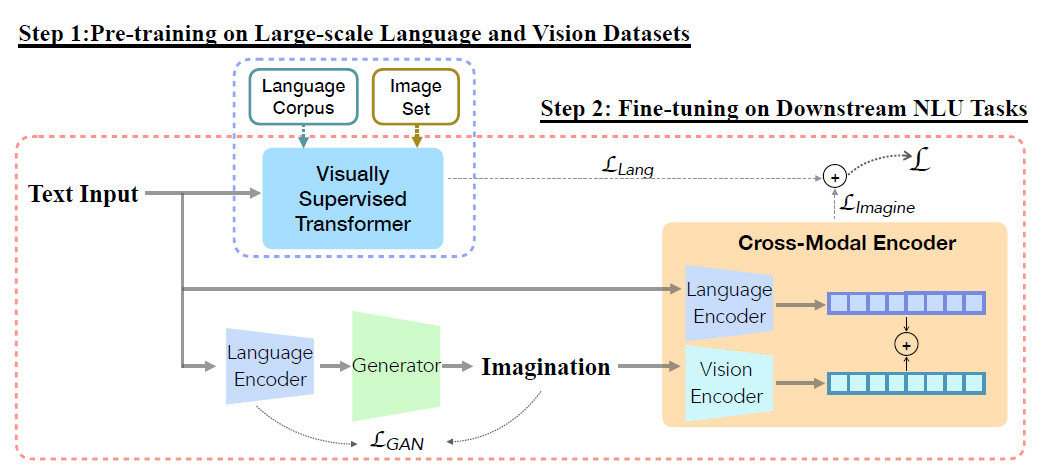
\includegraphics[width=1\linewidth]{figures/02-03-img-support-text/img-lu2022-01} 

}

\caption{From @lu2022imagination. The generator $G$ visualize imaginations close to the encoded texts by minimizing $\mathcal{L}_{GAN}$. The cross-modal encoder $E_c$ learns imagination-augmented language representation. Two-step learning procedure consists of: 1) pre-train a Transformer with visual supervision from large-scale language corpus and image set, 2) fine-tune the visually supervised pre-trained Transformer and the imagination-augmented cross-modal encoder on downstream tasks.}\label{fig:img-lu2022-01}
\end{figure}

This framework has two main components:

\begin{itemize}
\tightlist
\item
  the \textbf{imagination generator \(G\)}: given an input text \(x\), VQGAN (\citet{esser2021taming}) is used to render an ``imagination'' \(i\) of \(x\) and CLIP (\citet{radford2021learning}) is used to see how well the generated image \(i\) is aligned to the input text \(x\). This generative framework is known as VQGAN+CLIP
\item
  \textbf{Cross-modal Encoder \(E_c\)}: the input text and the rendered imagination are firstly encoded with a language and a visual encoder respectively and then CLIP is employed as cross-modal encoder with inputs being text-imagination pairs
\end{itemize}

The learning procedure is composed of two main steps (depicted in figure \ref{fig:img-lu2022-01}): the first step consists in the pre-training of a visually supervised Transformer. In particular, the Voken-Classification task described before is employed, alongside a masked language modeling task. This is the baseline model, where no information from the ``imagination'' procedure comes yet into play. The second step is the \emph{imagination-augmented fine-tuning} with two downstream datasets \(D\) (GLUE, \citet{wang2018glue} and SWAG, \citet{zellers2018swag}).\\
On one side, the visually-supervised Transformer (the baseline) relies only on the textual input during the fine-tuning phase and the following loss function is employed:

\[ \mathcal{L}_{Lang}=-\sum_{j=1}^{|D|}\sum_{k=1}^{K}y_{k}\ log\ p_{k}(d_{j}(t)|D) \]

On the other hand, the \emph{iACE} is trained to minimize the following cross-entropy loss:

\[ \mathcal{L}_{Imagine}=-\sum_{j=1}^{|D|}\sum_{k=1}^{K}y_{k}\ log\ p_{k}(d_{j}(t,v)|D) \]

with \(t\) and \(v\) being the textual and imagined features representations respectively, \(j\) indicates the \(j\)-th data sample in dataset belonging to dataset \(D\), \(K\) is the number of classes and \(p_k\) is the conditional distribution of \(d_j\).
Training takes place in a jointly fashion and both losses, the imagination-augmented one \(\mathcal{L}_{Imagine}\) and the pure language loss \(\mathcal{L}_{Lang}\) are linearly combined, with \(\lambda\) being a balance factor:

\[\mathcal{L}=\lambda\mathcal{L}_{Imagine}+(1-\lambda)\mathcal{L}_{Lang} \]

To sum up, this model-agnostic framework uses \emph{generated images} for visual supervision and could be integrated on top of pure language models (such as BERT) or visually supervised models (such as the Voken model, which uses Vokens, real images for visual supervision).

\hypertarget{was-it-worth}{%
\subsection{Was It Worth?}\label{was-it-worth}}

In this subchapter we investigated how visual inputs can support pure language models in capturing the semantics of words. We started with simple concatenation of linguistic and visual features and ended up with Transformer-based models, which are able to shape different word embeddings for the same word by taking into account also the context (the sentence). But now the question arises: with the addition of visual information, do we obtain word embeddings that are better than those from pure language models? In other words, is what we all have so far discussed worth? Well, as it is often the case in scientific research, the answer is: ``it depends!''

Individual evaluation of each single model might not be ideal because each model has its peculiarities and it is impractical to make a direct comparison among them. It is more useful to capture and discuss the themes which are common to many models, in order to understand their strengths and weaknesses. This is how we will proceed and we will also differentiate between evaluation before Transformers and evaluation after Transformers.

\hypertarget{evaluation-in-the-pre-transformers-era}{%
\subsubsection{Evaluation In The Pre-Transformers Era}\label{evaluation-in-the-pre-transformers-era}}

Before the advent of Transformers, the evaluation focus was on the degree of alignment between learned semantic representations (word embeddings) and representations by human speakers, in form of correlation between model-based and human-based word-similarity judgments. Three main types of similarity are usually considered:

\begin{itemize}
\item
  Semantic similarity, e.g.~``pasta is similar to rice''
\item
  Semantic relatedness, e.g.~``Bear is related to mountain''
\item
  Visual similarity, e.g.~``cucumbers look like zucchinis''
\end{itemize}

The evaluation pipeline could be summarized as follows:

\begin{figure}

{\centering 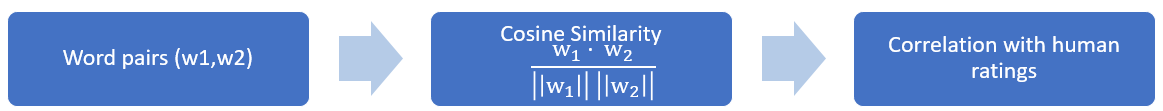
\includegraphics[width=1\linewidth]{figures/02-03-img-support-text/img-eval01} 

}

\caption{Pipeline for intrisinsic evaluation of semantic representations. In the first step, the cosine similarity between two word embeddings w1 and w2 is used as similariry measure and in a second step, the correlation with human speakers'assessment is computed to gauge the quality of the embeddings. The higher the correlation, the better the embeddings.}\label{fig:img-eval01}
\end{figure}

Word embeddings are vectors and to measure the degree of similarity between two vectors, the \emph{Cosine Similarity} is often used in the literature. In an ideal setting, we would have word embeddings with the following characteristics: if two words are semantically similar, the two embedding vectors should be similar and their cosine similarity should go towards 1. If the two words are unrelated, the embedding vectors should be orthogonal to each other and as a consequence, the cosine similarity should go towards zero. Lastly, if two words are negatively related, the two embedding vectors should point at opposite directions and the cosine similarity should go towards -1.
Once these similarity measures between word pairs are computed, in order to measure the quality of the embeddings several benchmarks can be employed, such as MEN (\citet{bruni2014multimodal}), WordSim353 (\citet{agirre2009study}) and SimLex999 (\citet{hill2015simlex}). These datasets could be described as collections of word pairs and associated similarity ratings by human speakers. Operationally, this means that real people were asked if a pair of words was related or not and to which degree, on a scale between -1 (negatively related) to +1 (semantically equivalent). The higher the correlation between the cosine similarity and the similarity judgments by humans, the higher the quality of the word embeddings. Having done this methodological premise, let's discuss the performance of these pre-Transformer models!

Since the goal of these models is to enhance pure language models with the addition of visual inputs, the baseline in the evaluation is always one (or more) pure language model(s). Well, do visually grounded embeddings outperform non-grounded ones? What emerges from virtually all papers is that visual grounding can actually help get a better semantic representation of \emph{concrete} concepts, such as ``cat'', ``table'', ``bicycle'', whereas they do not help much with the representation of abstract concepts such as ``love'' and ``peace''.

\begin{figure}

{\centering 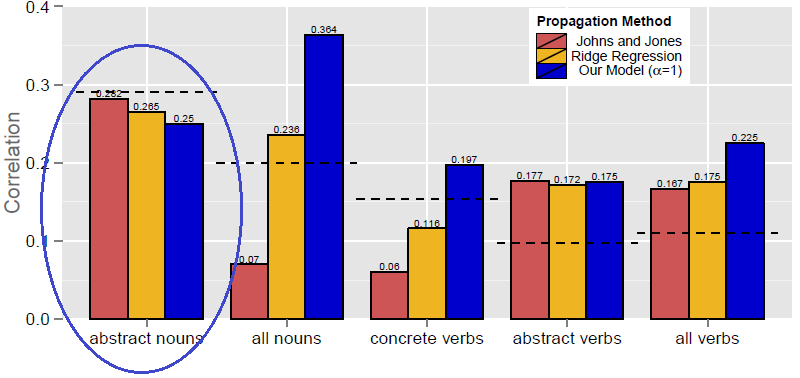
\includegraphics[width=1\linewidth]{figures/02-03-img-support-text/img-2014hill-01} 

}

\caption{From @hill2014learning: Each bar represents a different model settings and the dashed line indicates the pure linguistic benchmark model.}\label{fig:img-2014hill-01}
\end{figure}

In figure \ref{fig:img-2014hill-01} we can see that pure language models still perform better than models with visual inputs when it comes to the representation of abstract \emph{nouns}. Another example is \citet{kiela2017learning}: they found that their models perform better when tested on datasets with a higher degree of concreteness and the same conclusion is reached by \citet{collell2017imagined}, which state that visual information can empower the representations of concepts that are to a certain extent visual. To sum up, effective semantic representation of abstract concepts constitute the main limitation common to many of the models discussed in this section.

\hypertarget{evaluation-in-the-post-transformers-era}{%
\subsubsection{Evaluation In The Post-Transformers Era}\label{evaluation-in-the-post-transformers-era}}

A limitation of the \emph{intrinsic} evaluation metrics is the high degree of subjectivity: the \emph{similarity} between two concepts depends in many instances on the experience, cultural background and preferences of the human observers. This is why the evaluation focus has now shifted to a more \emph{extrinsic} dimension: how well do the models perform in downstream tasks? The problem of the ``lack of objectivity'' is thus solved because on downstream tasks there is no room for opinions. The datasets used to train the models are also different and the most widely used are:

\begin{itemize}
\tightlist
\item
  GLUE (\citet{wang2018glue}): 9 tasks, including single-sentence tasks (e.g.~sentiment analysis), similarity tasks (e.g.~paraphrasing), inference tasks (e.g.~textual entailment)
\item
  SQuAD (\citet{rajpurkar2016squad}): question/answer pairs
\item
  SWAG (\citet{zellers2018swag}): multiple choice questions about grounded situations
\end{itemize}

As previously discussed, many Transformer-based models have universal vocation: they are built to solve a heterogeneous range of tasks from the language and vision domain. If we thus consider only performance on pure language tasks, the following two tables from \citet{tan2020vokenization} are insightful:

\begin{figure}

{\centering 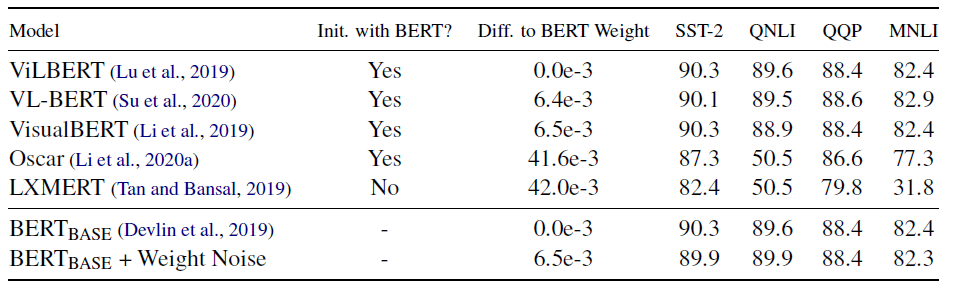
\includegraphics[width=1\linewidth]{figures/02-03-img-support-text/img-tan2020-02} 

}

\caption{From @tan2020vokenization. Results of vision-and-language pre-trained models (universal models) on GLUE tasks compared to baseline models (BERT).}\label{fig:img-tan2020-02}
\end{figure}

\begin{figure}

{\centering 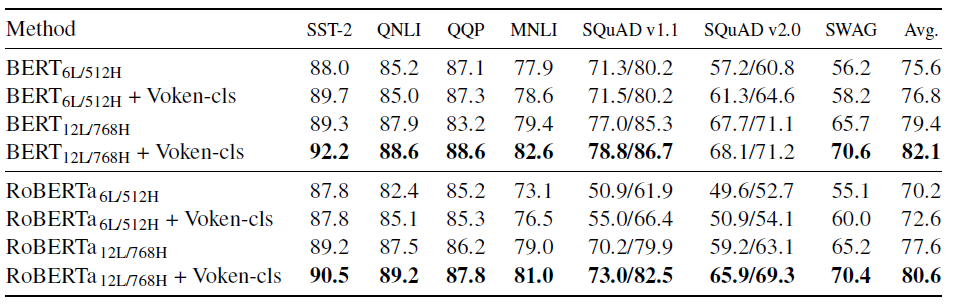
\includegraphics[width=1\linewidth]{figures/02-03-img-support-text/img-tan2020-03} 

}

\caption{From @tan2020vokenization. Fine-tuning results of different pre-trained models w/ or w/o the voken classification task (denoted as“Voken-cls”).}\label{fig:img-tan2020-03}
\end{figure}

It is straightforward: unlike in the pre-Transformers Era, where grounded word embeddings could improve performance over baselines, Transformer-based universal models \textbf{do not} outperform pure language models such as BERT or RoBERTa. Nonetheless, the addition of visual supervision (the Voken-Classification task) in the pre-training framework can boost performance above the level of pure language models.

\citet{pezzelle2021word} analyzed the \emph{intrinsic} quality of embeddings of some vision and language (``universal'') models:

\begin{figure}

{\centering 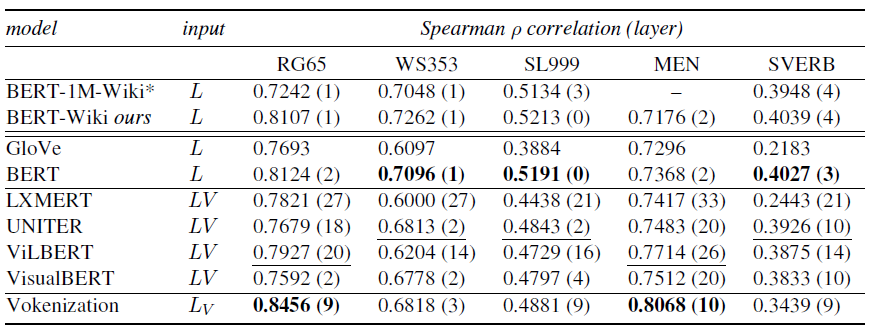
\includegraphics[width=1\linewidth]{figures/02-03-img-support-text/img-pezzele2021-01} 

}

\caption{From @pezzelle2021word. Spearman’s rank correlation between similarities computed with representations by all tested models and human similarity judgments in the five evaluation benchmarks.}\label{fig:img-pezzele2021-01}
\end{figure}

\begin{figure}

{\centering 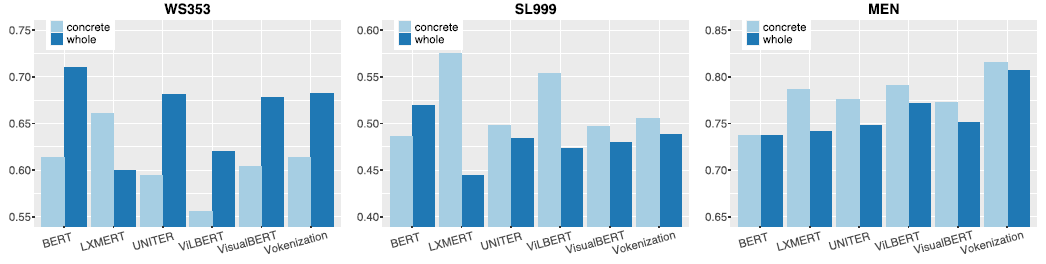
\includegraphics[width=1\linewidth]{figures/02-03-img-support-text/img-pezzele2021-02} 

}

\caption{From @pezzelle2021word. Correlation between model and human similarity ratings on WordSim353, SimLex999 and MEN. Each barplot reports results on both the whole benchmark and the most concrete subset of it.}\label{fig:img-pezzele2021-02}
\end{figure}

From this \emph{intrinsic} evaluation perspective (which was popular in the pre-Transformers Era), vision and language models do not generally outperform domain-specific models such as BERT and also in this case the only real competitor of pure language models is a model with visual supervision (again, Vokenization).\\
The bar plots depict correlation between human- and model-based similarity ratings, differentiating between the most \emph{concrete} concepts contained in a certain dataset\footnote{See \citet{brysbaert2014concreteness} for information on how \emph{concreteness} of a word can be estimated.} and the whole dataset (thus including more abstract concepts). The results confirm the trend: multimodal models are more effective than pure language models at representing concrete words but in many instances they still lag behind when it comes to more abstract concepts.

Last but not least, few words need to be spent on a topic which has been steadily gaining relevance: \textbf{Few-Shot Learning}. To train and test models, a large pool of paired images and texts is often needed and the creation of many of the datasets used in fine-tuning required a huge data collection effort, which had to be performed by human agents. This implies that the creation of such data pools can be very costly. For this reason, there is a growing interest in creating models able to cope with low-resource settings. This boils down to the question: can a model perform well on downstream tasks even with just a \emph{limited number} of training examples? The goal is actually once again, to mimic how humans learn: a person does not need to see one thousand pictures of a table, to be able to recognize a table\ldots{}

\begin{figure}

{\centering 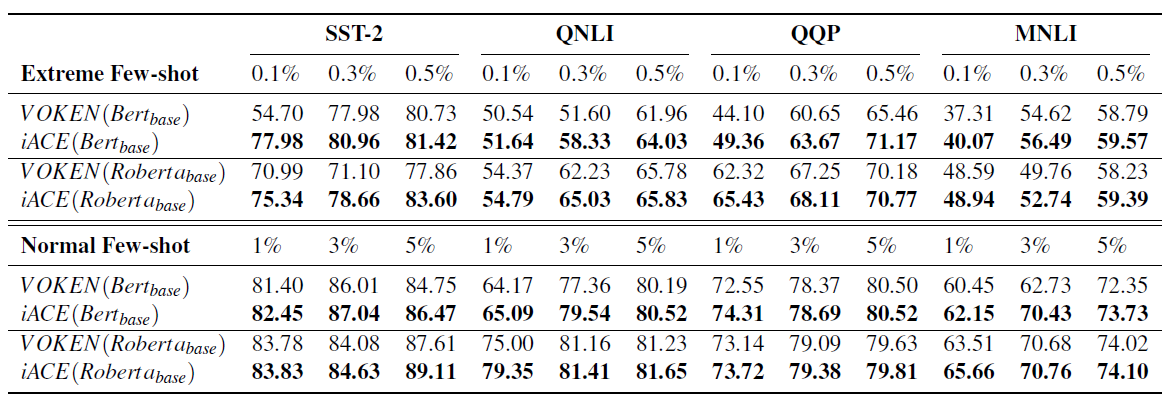
\includegraphics[width=1\linewidth]{figures/02-03-img-support-text/img-lu2022-02} 

}

\caption{From @lu2022imagination. Model-agnostic improvement in Few-shot Setting with GLUE benchmark.}\label{fig:img-lu2022-02}
\end{figure}

This table from \citet{lu2022imagination}, where models are trained using only up to 5\% of the training set, shows for example the ability for a model supervised with ``imagination'' (which was a generated visual representation of a certain textual input) to outperform models with only simple visual supervision (the Voken-model). This is just an example, but the ability to perform well in \emph{few-shot} settings has become the touchstone of the evaluation modern multimodal models.

\hypertarget{the-end-of-this-story}{%
\subsection{The End Of This Story}\label{the-end-of-this-story}}

We started this story with the \emph{Symbol Grounding Problem}, which affirms that to grasp the meaning of a word, the word has to be put in a context other than the pure linguistic one. We thus investigated some of the architectures proposed to ground words in a visual space in form of static images. The goal (hope) is to better capture the semantics of words, in form of better word embeddings, to be employed in heterogeneous tasks, from \emph{semantic-similarity} to downstream tasks, such as \emph{sentiment analysis}.\\
From this brief analysis it emerges that grounding words in images can actually improve the representation of \emph{concrete} concepts, whereas visual grounding does not seem to add value to pure language models when it comes to \emph{abstract} concepts. Nonetheless, forms of visual supervision like the \emph{Voken-Classification} task or the employment of generative models which allow to \emph{imagine} words, such as in the \emph{iACE-Framework}, might be the right way to bridge this gap.\\
The Transformers have been a revolution in the field of NLP and with their advent, the trend has now become to build models with pre-training tasks capable of generating powerful task-agnostic word representations. The knowledge gained with these tasks can be then transferred to downstream tasks with the goal to limit the amount of labeled data necessary to fine-tune models. Labeling data is indeed costly: this is why the ability of a model to generalize well when exposed to just few training examples has been steadily gaining importance as evaluation metric. This was the so called \emph{few-shot learning}. Moreover, Transformer-based models have ``universal vocation'': they tend to be multimodal and multi-task, encompassing vision, language and vision and language tasks. This idea might be appealing because humans learn by being exposed to a multitude of different inputs and tasks. But as we have seen, pure language models such as BERT tend to still outperform multimodal multi-task models. There is definitely room for improvement.\\
One might wonder whether the grounding of words in images is the right way to seek a better representation of words. Well, humans learn using all five senses and maybe the answer might be to incorporate in the models more heterogeneous perceptual information: not only static images but also videos, speech and the like. The debate is still open: the story \emph{goes on}\ldots{}

Last but not least, a mention needs to be made on concrete applications of these image-empowered word-embeddings. The use of images to support linguistic models has been experimented in several fields, from \emph{Dialogue Response Generation} (e.g.~\citet{sun2021multimodal}) to \emph{Machine Translation}, where for example \citet{ive2019distilling} found images to improve the quality of translation when the textual context is generic and/or ambiguous. The number of potential applications of the models described in this subchapter is growing steadily in the scientific community. But this is yet \emph{another} story\ldots{}

\hypertarget{appendix-selected-models---summary}{%
\subsection{Appendix: Selected Models - Summary}\label{appendix-selected-models---summary}}

The following table contains a summary of selected language models augmented with visual components. For each model, the following information are reported:

\begin{itemize}
\item
  Pure language model and pretraining data
\item
  Visual features and pretraining data
\item
  Fusion strategy of the two modalities
\item
  Benchmarks/baselines for evaluation:

  \(\color{green}\blacktriangle\) better performance over baseline(s)\\
  \(\color{orange}\bullet\) mixed performance results over baseline(s)\\
  \(\color{red}\blacktriangledown\) worse performance over baseline(s)\\
\end{itemize}

The table is available in a more readable format \href{Table-ch2-3-final.pdf}{here}.

\begin{longtable}[]{@{}llllllllll@{}}
\toprule
\begin{minipage}[b]{0.00\columnwidth}\raggedright
Year\strut
\end{minipage} & \begin{minipage}[b]{0.06\columnwidth}\raggedright
Paper\strut
\end{minipage} & \begin{minipage}[b]{0.04\columnwidth}\raggedright
Language model (LM)\strut
\end{minipage} & \begin{minipage}[b]{0.02\columnwidth}\raggedright
LM-Pre-training sources\strut
\end{minipage} & \begin{minipage}[b]{0.07\columnwidth}\raggedright
Visual elements (IMG)\strut
\end{minipage} & \begin{minipage}[b]{0.05\columnwidth}\raggedright
IMG-Pre-training sources\strut
\end{minipage} & \begin{minipage}[b]{0.25\columnwidth}\raggedright
Multimodal representation and model description\strut
\end{minipage} & \begin{minipage}[b]{0.08\columnwidth}\raggedright
Testset/Fine-tuning\strut
\end{minipage} & \begin{minipage}[b]{0.05\columnwidth}\raggedright
Baseline(s)/model settings/comparison to other models\strut
\end{minipage} & \begin{minipage}[b]{0.13\columnwidth}\raggedright
Results\strut
\end{minipage}\tabularnewline
\midrule
\endhead
\begin{minipage}[t]{0.00\columnwidth}\raggedright
2014\strut
\end{minipage} & \begin{minipage}[t]{0.06\columnwidth}\raggedright
Bruni, Elia, Nam-Khanh Tran, and Marco Baroni. ``Multimodal distributional semantics.''~Journal of artificial intelligence research~49 (2014): 1-47.\strut
\end{minipage} & \begin{minipage}[t]{0.04\columnwidth}\raggedright
Distributional model expressed as a matrix with rows as ``semantic vectors'' representing the meaning of a set of target words. The model is based on co-occurrence counts of words (as a result, the matrix is a squared one).\strut
\end{minipage} & \begin{minipage}[t]{0.02\columnwidth}\raggedright
- ukWaC, 1.9B tokens- Wackypedia, 820M tokens.\strut
\end{minipage} & \begin{minipage}[t]{0.07\columnwidth}\raggedright
(i) Local descriptors to extract low-level visual features(ii) Assign local descriptors to cluster of visual words (bag of words) to build the vector representation of an image(iii) Sum up visual words co-occurrence to across all images/instances to get co-occurrence counts related to a target word (the resulting matrix is a squared one).\strut
\end{minipage} & \begin{minipage}[t]{0.05\columnwidth}\raggedright
ESP-Game dataset, 100K images.\strut
\end{minipage} & \begin{minipage}[t]{0.25\columnwidth}\raggedright
Only words for which there is a related image are considered.Two steps to build multimodal representations:(i) Textual and visual matrices are concatenated and projected into a common latent multimodal space with a singular value decomposition. From this matrix, the ``textual mixed matrix'' and the ``visual mixed matrix'' are extracted(ii) Association between words is assessed with cosine similarityTwo fusion methods to estimate similarity of pairs:- Feature level fusion: linear combination of textual and visual mixed matrix and then similarity estimation- Scoring level fusion: word similarity computed on both textual and visual mixed matrices separately and then the final score is a linear combination of the twoIn both methods the weights in the linear combinations are hyperparameter.\strut
\end{minipage} & \begin{minipage}[t]{0.08\columnwidth}\raggedright
- WordSim353- MEN.\strut
\end{minipage} & \begin{minipage}[t]{0.05\columnwidth}\raggedright
- Text mixed embeddings only- Visual mixed embeddings only- Equally weighted versions of feature and scoring level fusion model settings- Several ``fine tuned'' versions of fusion and scoring level fusion model settings.\strut
\end{minipage} & \begin{minipage}[t]{0.13\columnwidth}\raggedright
\(\color{green}\blacktriangle\)Multimodal word representations enhance performance of purely textual or visual embeddings\(\color{orange}\bullet\)No alternative model used as a means of comparison.\strut
\end{minipage}\tabularnewline
\begin{minipage}[t]{0.00\columnwidth}\raggedright
2014\strut
\end{minipage} & \begin{minipage}[t]{0.06\columnwidth}\raggedright
Hill, Felix, and Anna Korhonen. ``Learning abstract concept embeddings from multi-modal data: Since you probably can't see what I mean.''~Proceedings of the 2014 Conference on Empirical Methods in Natural Language Processing (EMNLP). 2014.\strut
\end{minipage} & \begin{minipage}[t]{0.04\columnwidth}\raggedright
Skipgram.\strut
\end{minipage} & \begin{minipage}[t]{0.02\columnwidth}\raggedright
400m word Text8 Corpus.\strut
\end{minipage} & \begin{minipage}[t]{0.07\columnwidth}\raggedright
Mapping of words w to a bag of perceptual features b(w), extracted from external sources and encoded in an associative array P. Generation of pseudo sentences based on these perceptual features to be fed into the language model.\strut
\end{minipage} & \begin{minipage}[t]{0.05\columnwidth}\raggedright
- ESP-Game (100K images)- CSLB Property Norms.\strut
\end{minipage} & \begin{minipage}[t]{0.25\columnwidth}\raggedright
~Extension of the Skipgram injecting perceptual information by generating pseudo-sentences based on a bag-of-visual-words. A hyperparameter \(\alpha\) controls the level of perceptual information relative to linguistic input.\strut
\end{minipage} & \begin{minipage}[t]{0.08\columnwidth}\raggedright
USF Dataset.\strut
\end{minipage} & \begin{minipage}[t]{0.05\columnwidth}\raggedright
- Concatenation of linguistic and perceptual features- Canonical Correlation Analysis applied on vectors of both modalities- SVD of matrix of concatenated multimodal representations.\strut
\end{minipage} & \begin{minipage}[t]{0.13\columnwidth}\raggedright
\(\color{green}\blacktriangle\)Concepts, which can directly be represented in the perceptual modality (e.g.~concrete verbs and nouns)\(\color{green}\blacktriangle\)Propagation of perceptual input from concrete concepts (nouns and verbs) to enhance the representation of abstract verbs, those for which no direct representation in the visual space is available\(\color{red}\blacktriangledown\)Abstract nouns (for which is more difficult to find a concrete visual representation) are still more efficiently learned from language-only models.\strut
\end{minipage}\tabularnewline
\begin{minipage}[t]{0.00\columnwidth}\raggedright
2014\strut
\end{minipage} & \begin{minipage}[t]{0.06\columnwidth}\raggedright
Douwe Kiela and Léon Bottou. 2014. Learning Image Embeddings using Convolutional Neural Networks for Improved Multi-Modal Semantics. In Proceedings of the 2014 Conference on Empirical Methods in Natural Language Processing (EMNLP), pages 36--45, Doha, Qatar. Association for Computational Linguistics.\strut
\end{minipage} & \begin{minipage}[t]{0.04\columnwidth}\raggedright
Skipgram.\strut
\end{minipage} & \begin{minipage}[t]{0.02\columnwidth}\raggedright
- Text8 Corpus (400M words)- British National Corpus (100M words).\strut
\end{minipage} & \begin{minipage}[t]{0.07\columnwidth}\raggedright
Seventh layer of a CNN to extract 6144-d features vectors for images, obtained in two ways:- CNN-Mean (average of all features vectors representing images)- CNN-Max (component-wise maximum of all features vectors)\strut
\end{minipage} & \begin{minipage}[t]{0.05\columnwidth}\raggedright
- ImageNet (12.5M images)- Esp-Game (100K images).\strut
\end{minipage} & \begin{minipage}[t]{0.25\columnwidth}\raggedright
Concatenation of visual and textual embeddings.\strut
\end{minipage} & \begin{minipage}[t]{0.08\columnwidth}\raggedright
- MEN- WordSim353 (it captures not only ``relatedness'' but also ``similarity''.\strut
\end{minipage} & \begin{minipage}[t]{0.05\columnwidth}\raggedright
- Skipgram (text-only baseline)- Embeddings - visual only.\strut
\end{minipage} & \begin{minipage}[t]{0.13\columnwidth}\raggedright
\(\color{green}\blacktriangle\)CNN-Mean better on MEN: averaging might capture relatedness better. CNN-Max better on WordSim353.\strut
\end{minipage}\tabularnewline
\begin{minipage}[t]{0.00\columnwidth}\raggedright
2014\strut
\end{minipage} & \begin{minipage}[t]{0.06\columnwidth}\raggedright
Silberer, Carina, and Mirella Lapata. ``Learning grounded meaning representations with autoencoders.''~Proceedings of the 52nd Annual Meeting of the Association for Computational Linguistics (Volume 1: Long Papers). 2014.\strut
\end{minipage} & \begin{minipage}[t]{0.04\columnwidth}\raggedright
Vectors of textual attributes are extracted.\strut
\end{minipage} & \begin{minipage}[t]{0.02\columnwidth}\raggedright
- McRae et al.'s (2005).\strut
\end{minipage} & \begin{minipage}[t]{0.07\columnwidth}\raggedright
Vectors of visual attributes are extracted.\strut
\end{minipage} & \begin{minipage}[t]{0.05\columnwidth}\raggedright
Same dataset as in Silberer et al.~(2013): taxonomy of 636 visualattributes (e.g., has wings, made of wood) andnearly 700K images from ImageNet (Deng et al.,2009) describing more than 500 of McRae et al.'s(2005) nouns.\strut
\end{minipage} & \begin{minipage}[t]{0.25\columnwidth}\raggedright
Stacked (denoising) autoencoders for each single modality and the outputs are concatenated and fed to a stacked bimodal autoencoder which map the inputs to a joint hidden layer.\strut
\end{minipage} & \begin{minipage}[t]{0.08\columnwidth}\raggedright
With McRae et al.'s (2005), two tasks:- word similarity- word categorization.\strut
\end{minipage} & \begin{minipage}[t]{0.05\columnwidth}\raggedright
- Unimodal autoencoders only- Kernelized Canonical Correlation, Hardoon et al.~(2004)- Bruni et al.~(2014).\strut
\end{minipage} & \begin{minipage}[t]{0.13\columnwidth}\raggedright
\(\color{green}\blacktriangle\)Bimodal models outperform unimodal ones\(\color{red}\blacktriangledown\)Training is on attribute-based inputs. Not widely used in the field.\strut
\end{minipage}\tabularnewline
\begin{minipage}[t]{0.00\columnwidth}\raggedright
2015\strut
\end{minipage} & \begin{minipage}[t]{0.06\columnwidth}\raggedright
Lazaridou, Angeliki, Nghia The Pham, and Marco Baroni. ``Combining language and vision with a multimodal skip-gram model.''~arXiv preprint arXiv:1501.02598~(2015).\strut
\end{minipage} & \begin{minipage}[t]{0.04\columnwidth}\raggedright
Skipgram.\strut
\end{minipage} & \begin{minipage}[t]{0.02\columnwidth}\raggedright
Wikipedia 2009, 800M Tokens.\strut
\end{minipage} & \begin{minipage}[t]{0.07\columnwidth}\raggedright
Visual information for 5100 words with an entry in ImageNet, occur \textgreater500 times in the text corpus and have a~ concreteness score \(\geq\) 0.5; sample 100 images for each word and extract a 4096-d array with a CNN; average the vectors of 100 pictures associated to each word to get visual representation.\strut
\end{minipage} & \begin{minipage}[t]{0.05\columnwidth}\raggedright
ImageNet.\strut
\end{minipage} & \begin{minipage}[t]{0.25\columnwidth}\raggedright
The objective function is a linear composition of the language objective L-ling from the Skipgram and a visual objective L-vision.For the L-vision objective two variants are proposed:- MM Skipgram A (MMSA): aligning vectors of visual and linguistic representations (1:1 correspondence assumed)- MM Skipgram B (MMSB): estimate a cross-modal mapping matrix from linguistic onto visual representations.\strut
\end{minipage} & \begin{minipage}[t]{0.08\columnwidth}\raggedright
- MEN- SemSim- VisSim.\strut
\end{minipage} & \begin{minipage}[t]{0.05\columnwidth}\raggedright
- Kiela and Bottou (2014)- Bruni et al.~(2014)- Silberer \& Lapata (2014)- Skipgram (text-only baseline)- Embeddings - visual only- Concatenation- SVD.\strut
\end{minipage} & \begin{minipage}[t]{0.13\columnwidth}\raggedright
\(\color{green}\blacktriangle\)Both MMSA and MMSB better than simpler models (linguistic/vision only, concatenation SVD)\(\color{orange}\bullet\)MMSA and MMSB competitive in relatedness and visual similarity, despite having often less training data than other models\(\color{orange}\bullet\)Visual grounding less effective with abstract words\strut
\end{minipage}\tabularnewline
\begin{minipage}[t]{0.00\columnwidth}\raggedright
2017\strut
\end{minipage} & \begin{minipage}[t]{0.06\columnwidth}\raggedright
Collell, Guillem, Ted Zhang, and Marie-Francine Moens. ``Imagined visual representations as multimodal embeddings.''~Proceedings of the AAAI Conference on Artificial Intelligence. Vol. 31. No.~1. 2017.\strut
\end{minipage} & \begin{minipage}[t]{0.04\columnwidth}\raggedright
300-d GloVe.\strut
\end{minipage} & \begin{minipage}[t]{0.02\columnwidth}\raggedright
Common Crawl corpus, 840B tokens, 2.2M words.\strut
\end{minipage} & \begin{minipage}[t]{0.07\columnwidth}\raggedright
To extract visual features, the last hidden layer of~ a CNN is taken. For each concept, two different ways to combine the extracted visual features:- Averaging (averaging of al features vectors)- Maxpooling (component-wise maximum).\strut
\end{minipage} & \begin{minipage}[t]{0.05\columnwidth}\raggedright
Imagenet.\strut
\end{minipage} & \begin{minipage}[t]{0.25\columnwidth}\raggedright
Mapping from language to vision. No need of 1:1 correspondence between linguistic and visual inputs. Two different mappings are considered:- Linear (MAP-Clin)- Neural Network (MAP-Cnn).\strut
\end{minipage} & \begin{minipage}[t]{0.08\columnwidth}\raggedright
- MEN- WordSim353- SemSim- Simlex999-SimVerb3500- VisSim.\strut
\end{minipage} & \begin{minipage}[t]{0.05\columnwidth}\raggedright
- Kiela and Bottou (2014)- Lazaridou et al.~(2015)- Silberer \& Lapata (2014)- GloVe (text-only baseline)- Concatenation.\strut
\end{minipage} & \begin{minipage}[t]{0.13\columnwidth}\raggedright
\(\color{green}\blacktriangle\)Outperformance in all instances where words have associated images in the training set\(\color{red}\blacktriangledown\)Performance on the zero-shot learning still inferior in many instances to the textual baselines.\strut
\end{minipage}\tabularnewline
\begin{minipage}[t]{0.00\columnwidth}\raggedright
2018\strut
\end{minipage} & \begin{minipage}[t]{0.06\columnwidth}\raggedright
Kiela, Douwe, et al.~``Learning visually grounded sentence representations.''~arXiv preprint arXiv:1707.06320~(2017).\strut
\end{minipage} & \begin{minipage}[t]{0.04\columnwidth}\raggedright
- GloVe for word embeddings- Bidirectional LSTM for sentence representation.\strut
\end{minipage} & \begin{minipage}[t]{0.02\columnwidth}\raggedright
WebCrawl\strut
\end{minipage} & \begin{minipage}[t]{0.07\columnwidth}\raggedright
Image features obtained from the final layer of a ResNet-101.\strut
\end{minipage} & \begin{minipage}[t]{0.05\columnwidth}\raggedright
MS COCO.\strut
\end{minipage} & \begin{minipage}[t]{0.25\columnwidth}\raggedright
Word embeddings are projected to a ground space with a linear mapping. Linear mapping and Bi-LSTM are trained jointly.Three methods to ground sentences in images, captions or both:- Cap2Img: predict latent features of an image from its caption by mapping the (final) hidden state h(T) of the Bi-LSTM to the latent representation of the image. A ranking loss is to be minimized- Cap2Cap: given the caption pair (x,y) describing the same image, the goal is to maximize the joint probability of y given x. Negative log-likelihood as loss.- Cap2Both: Goal is to minimize the two loss functions above.In another setting, grounded and sentence-only (Skipthought) representations are concatenated with layer normalization~ to get the final sentence representations. Goal is to include information on less concrete concepts which are not likely to be represented in image-captioning databases but are present in language corpora.\strut
\end{minipage} & \begin{minipage}[t]{0.08\columnwidth}\raggedright
Intrinsic evaluation of word embeddings:- MEN- SimLex 999- Rare Words- WordSim-353Extrinsic evaluations:- Movie review Sentiment (MR)- Product reviews (CR)- Subjectivity classification (SUBJ)- Opinion polarity (MPQA)- Paraphrase identification (MSRP)- Sentiment classification (SST)- SNLI (Entailment)- SICK (Entailment).\strut
\end{minipage} & \begin{minipage}[t]{0.05\columnwidth}\raggedright
- Skipthought (text-only baseline).\strut
\end{minipage} & \begin{minipage}[t]{0.13\columnwidth}\raggedright
\(\color{green}\blacktriangle\)Word embeddings are of higher quality than those obtained with GloVe, measured on the following similarity benchmarks: MEN, SimLex999, Rare Words and WordSim-353\(\color{green}\blacktriangle\)In extrinsic evaluations, grounding increases performance but it is not clear which one of the three grounding strategies considered is dominant\(\color{orange}\bullet\)Performance seems to be driven in a smaller amount of instances by a larger number of parameters rather than effectiveness of grounding\(\color{orange}\bullet\)Performance is better when dataset have a higher level of concreteness.\strut
\end{minipage}\tabularnewline
\begin{minipage}[t]{0.00\columnwidth}\raggedright
2020\strut
\end{minipage} & \begin{minipage}[t]{0.06\columnwidth}\raggedright
Bordes, Patrick, et al.~``Incorporating visual semantics into sentence representations within a grounded space.''~arXiv preprint arXiv:2002.02734~(2020).\strut
\end{minipage} & \begin{minipage}[t]{0.04\columnwidth}\raggedright
- Skipthought.\strut
\end{minipage} & \begin{minipage}[t]{0.02\columnwidth}\raggedright
Toronto Book Corpus: 11M books, 74M ordered sentences, 13 words per sentence on average.\strut
\end{minipage} & \begin{minipage}[t]{0.07\columnwidth}\raggedright
Processing of visual elements with a pre-trained Inception v3 network (Szegedy et al., 2016).\strut
\end{minipage} & \begin{minipage}[t]{0.05\columnwidth}\raggedright
MS COCO: 118K/5K/41K (train/val/test) images.\strut
\end{minipage} & \begin{minipage}[t]{0.25\columnwidth}\raggedright
The objective function is composed of:- a textual objective Lt- a grounding objective Lg, which among its parameters has also those of the textual objective, which in turn profit from both objective functions.Lg is not applied directly on the sentence embeddings; it is trained on an intermediate space called the ``grounded space''. The sentence embeddings are projected to the grounded space with the projection function being a multi-layer perceptron. The goal is to move away from the 1:1 correspondence between textual and visual space.Lg the~ can be decomposed in two components, whose individual contribution is controlled by two hyperparameters:- Cluster Information (Cg): sentences associated with the same image(s) should be similar. The visual space is thus used to asses sentence similarity. The~ Max-margin ranking loss is used- Perceptual information (Pg): similarity between sentences in the grounded space~ should be correlated with similarity between corresponding images in the visual space. The loss is based on the negative Pearson correlation.Model scenarios include many compositions of the above mentioned elements.\strut
\end{minipage} & \begin{minipage}[t]{0.08\columnwidth}\raggedright
Intrinsic evaluation of word embeddings:- STS- SICKExtrinsic evaluations:- Movie review Sentiment (MR)- Product reviews (CR)- Subjectivity classification (SUBJ)- Opinion polarity (MPQA)- Paraphrase identification (MSRP)- Sentiment classification (SST)- SNLI (Entailment)- SICK (Entailment).\strut
\end{minipage} & \begin{minipage}[t]{0.05\columnwidth}\raggedright
- Skipthought (text-only baseline)For extrinsic evaluations:- Kiros et al.~(2014)- Kiela et al.~(2018)- Lazaridou et al.~(2015) - cross-modal- Collell et al.~(2017) - sequential/concatenation.\strut
\end{minipage} & \begin{minipage}[t]{0.13\columnwidth}\raggedright
\(\color{green}\blacktriangle\)Word embeddings are~ better than the textual benchmark for data with a high level of concreteness and are similar in performance with respect to more abstract concepts\(\color{green}\blacktriangle\)Projections on the grounded space are more effective than cross-modal projection and concatenation\(\color{orange}\bullet\)Not always best performance on entailment tasks (benchmarks SNLI, SICK).\strut
\end{minipage}\tabularnewline
\begin{minipage}[t]{0.00\columnwidth}\raggedright
2020\strut
\end{minipage} & \begin{minipage}[t]{0.06\columnwidth}\raggedright
Tan, Hao, and Mohit Bansal. ``Vokenization: Improving language understanding with contextualized, visual-grounded supervision.''~arXiv preprint arXiv:2010.06775~(2020).\strut
\end{minipage} & \begin{minipage}[t]{0.04\columnwidth}\raggedright
BERT, but it can be adapted to any language model (through Revokenization).\strut
\end{minipage} & \begin{minipage}[t]{0.02\columnwidth}\raggedright
English Wikipedia.\strut
\end{minipage} & \begin{minipage}[t]{0.07\columnwidth}\raggedright
ResNeXt.\strut
\end{minipage} & \begin{minipage}[t]{0.05\columnwidth}\raggedright
MS COCO.\strut
\end{minipage} & \begin{minipage}[t]{0.25\columnwidth}\raggedright
Language model with visual supervision. Each token in a sentence obtains a corresponding image (voken) assigned from a finite set of images. The voken is the image which maximize a Relevance Score Function between a token and all images in the aforementioned finite set of images. With this token-voken pairs a voken classification pre-training task is performed that can be built in pure language models alongside other pre-training tasks such MLM or Next-Sentence Prediction.\strut
\end{minipage} & \begin{minipage}[t]{0.08\columnwidth}\raggedright
- GLUE (only SST-2, QNLI, QQP, MNLI)- SQuAD- SWAG.\strut
\end{minipage} & \begin{minipage}[t]{0.05\columnwidth}\raggedright
- BERT (various versions)- VilBert- VL-BERT- VisualBERT- Oscar- LXMERT.\strut
\end{minipage} & \begin{minipage}[t]{0.13\columnwidth}\raggedright
\(\color{green}\blacktriangle\) Improvement over the purely self-supervised language model on multiple language tasks.\strut
\end{minipage}\tabularnewline
\begin{minipage}[t]{0.00\columnwidth}\raggedright
2021\strut
\end{minipage} & \begin{minipage}[t]{0.06\columnwidth}\raggedright
Hu, Ronghang, and Amanpreet Singh. ``Unit: Multimodal multitask learning with a unified transformer.''~Proceedings of the IEEE/CVF International Conference on Computer Vision. 2021.\strut
\end{minipage} & \begin{minipage}[t]{0.04\columnwidth}\raggedright
BERT-base with a learned task-specific vector (to capture task-specific information) as additional input, which is positioned at the beginning of the embedded token sequence.\strut
\end{minipage} & \begin{minipage}[t]{0.02\columnwidth}\raggedright
Pretrained version of the embeddings\strut
\end{minipage} & \begin{minipage}[t]{0.07\columnwidth}\raggedright
CNN (ResNet-50) to extract visual features map + transformer encoder to encode the features map to a set of hidden states. A learned task-task specific vector (to capture task-specific information) is concatenated to the beginning of the visual feature list before entering the encoder (architecture inspired by DETR).\strut
\end{minipage} & \begin{minipage}[t]{0.05\columnwidth}\raggedright
- MS COCO- Visual Genome.\strut
\end{minipage} & \begin{minipage}[t]{0.25\columnwidth}\raggedright
To both modalities is then applied a domain agnostic transformer architecture. As input the transformer takes the hidden states of either language or visual encoders or concatenation of both together with a task specific query embedding sequence. Self attention is applied in each layer among decoder hidden states and cross attention is applied to the encoded input modalities. The output is a set of decoded hidden states to which a task-specific head is applied (two-layer MPLP with GeLU activation and cross entropy loss).Training is done jointly on multiple tasks. At each training iteration, a task is randomly selected.Three settings (third one is the model described above):1.) Single-task training: each model is trained separately on each task2.) Multi-task training with separate decoders: a specific decoder for each task and jointly trained on all tasks3.) Multi-task training with shared decoder. In this setting, there are still task-specific heads for each task.\strut
\end{minipage} & \begin{minipage}[t]{0.08\columnwidth}\raggedright
Extrinsic evaluation.: GLUE:- QNLI- QQP- MNLI- SST2.\strut
\end{minipage} & \begin{minipage}[t]{0.05\columnwidth}\raggedright
BERT (text-only baseline).\strut
\end{minipage} & \begin{minipage}[t]{0.13\columnwidth}\raggedright
\(\color{green}\blacktriangle\)Model setting (1), single task training, outperforms all other settings and is comparable to the text-only baseline\(\color{red}\blacktriangledown\)Model setting (3), domain-agnostic, multi-task training with shared decoder across modalities exhibits a lower performance compared to domain-specific transformer models like BERT, the text-only baseline.\strut
\end{minipage}\tabularnewline
\begin{minipage}[t]{0.00\columnwidth}\raggedright
2021\strut
\end{minipage} & \begin{minipage}[t]{0.06\columnwidth}\raggedright
Shahmohammadi, Hassan, Hendrik Lensch, and R. Harald Baayen. ``Learning zero-shot multifaceted visually grounded word embeddings via multi-task training.''~arXiv preprint arXiv:2104.07500~(2021).\strut
\end{minipage} & \begin{minipage}[t]{0.04\columnwidth}\raggedright
- GloVe, 300d, 2.2M words- fastText, 300d, 2M.\strut
\end{minipage} & \begin{minipage}[t]{0.02\columnwidth}\raggedright
Pretrained version of the embeddings\strut
\end{minipage} & \begin{minipage}[t]{0.07\columnwidth}\raggedright
Image vectors obtained by transferring the penultimate layer of pretrained Inception-V3 trained on ImageNet. A neural network with one hidden layer and tanh activation is used to~ project the image vectors into the initial hidden state of the GRUs employed in the model.\strut
\end{minipage} & \begin{minipage}[t]{0.05\columnwidth}\raggedright
MS COCO.\strut
\end{minipage} & \begin{minipage}[t]{0.25\columnwidth}\raggedright
Given embeddings originating from a pretrained text-only model, the goal is to generate a mapping matrix M to ground word embeddings visually (the mapping matrix is used in both directions, to map text to grounded space and to map grounded embeddings back to the textual space)This is obtained by performing three different tasks:(i) Next word prediction with a GRU, given previous words in the sentence provided as image caption, together with the~ related image embedding vector(ii) Same as (i) but the sentence is provided backwards to another GRU(iii) Binary classification task if the representation of a given sentence in the grounded space obtained from (i) and (ii) matched the associated image.\strut
\end{minipage} & \begin{minipage}[t]{0.08\columnwidth}\raggedright
Limited to intrinsic evaluation:- MEN- SimLex999- Rare Words- MTurk771- WordSim353- SimVerb3500.\strut
\end{minipage} & \begin{minipage}[t]{0.05\columnwidth}\raggedright
- GloVe (text-only baseline)- fastText (text-only baseline)- Collell et al.~(2017)- Park \& Myaeng (2017)- Kiros et al.~(2018)- Kiela et al.~(2018).\strut
\end{minipage} & \begin{minipage}[t]{0.13\columnwidth}\raggedright
\(\color{green}\blacktriangle\)Textual baselines and related models are outperformed and the model seems to improve the textual vector space by aligning it with real-world relations from the images (similarity appears to be favoured by the model over relatedness)\(\color{green}\blacktriangle\)Embeddings related to less concrete words exhibit good quality compared to baselines.\strut
\end{minipage}\tabularnewline
\begin{minipage}[t]{0.00\columnwidth}\raggedright
2022\strut
\end{minipage} & \begin{minipage}[t]{0.06\columnwidth}\raggedright
Hsu, Chan-Jan, Hung-yi Lee, and Yu Tsao. ``XDBERT: Distilling Visual Information to BERT from Cross-Modal Systems to Improve Language Understanding.''~arXiv preprint arXiv:2204.07316~(2022).\strut
\end{minipage} & \begin{minipage}[t]{0.04\columnwidth}\raggedright
- BERT- ELECTRA.\strut
\end{minipage} & \begin{minipage}[t]{0.02\columnwidth}\raggedright
Wikipedia.\strut
\end{minipage} & \begin{minipage}[t]{0.07\columnwidth}\raggedright
CLIP as image-text matching system: two components, a text encoder (CLIP-T) and an image encoder (CLIP-ViT).\strut
\end{minipage} & \begin{minipage}[t]{0.05\columnwidth}\raggedright
not specified.\strut
\end{minipage} & \begin{minipage}[t]{0.25\columnwidth}\raggedright
3 adaptive tasks:- Joint Masked Language Modelling (MLM)- Same Sentence Prediction (MATCH)- CLIP Token ClassificationAfter that, concatenation with cross-modal encoder is performed.\strut
\end{minipage} & \begin{minipage}[t]{0.08\columnwidth}\raggedright
- GLUE- SWAG- READ.\strut
\end{minipage} & \begin{minipage}[t]{0.05\columnwidth}\raggedright
- BERT- ELECTRA.\strut
\end{minipage} & \begin{minipage}[t]{0.13\columnwidth}\raggedright
\(\color{green}\blacktriangle\)Better performance than pure language models, in particular in smaller datasets, which suggests that visual inputs improve generalization when the amount of training data is limited.\strut
\end{minipage}\tabularnewline
\begin{minipage}[t]{0.00\columnwidth}\raggedright
2022\strut
\end{minipage} & \begin{minipage}[t]{0.06\columnwidth}\raggedright
Lu, Yujie, et al.~``Imagination-Augmented Natural Language Understanding.''~arXiv preprint arXiv:2204.08535~(2022).\strut
\end{minipage} & \begin{minipage}[t]{0.04\columnwidth}\raggedright
- BERT-base- RoBERTa.\strut
\end{minipage} & \begin{minipage}[t]{0.02\columnwidth}\raggedright
Wikipedia.\strut
\end{minipage} & \begin{minipage}[t]{0.07\columnwidth}\raggedright
Same as in VOKENIZATION paper.\strut
\end{minipage} & \begin{minipage}[t]{0.05\columnwidth}\raggedright
MS COCO.\strut
\end{minipage} & \begin{minipage}[t]{0.25\columnwidth}\raggedright
The framework iACE is composed of two modules:1.) Imagination generator G: for each text input, VQGAN generates an ``imagined visual'' and CLIP is used to test how the generated image corresponds to the text and encodes the text and the image in a cross-modal embedding space and the objective function Lgan is to minimize the distance between these two embeddings2.) Imagination augmented cross-modal encoder. Specifically, CLIP is used, with the embeddings from the textual and visual encoder (fed with the visualized imaginations)~ within CLIP are then ``late fused''. The output is a set of ``imagination-augmented'' language representations.Learning procedure:1.) pre-training of a visually-supervised transformer following the Vokenization method2.) Imagination-augmented fine tuning, composed of two losses to be minimized:(i) L-imagine where the iACE framework tries to minimize the cross-entropy loss based on text embeddings and visually imagination embeddings, given a testsets and a number of classes to predict(ii)L-lang, where the visually supervised transformer only relies on textual inputsThe ``imagination-augmented'' is a composition of (i) and (ii) and the relative contribution of each loss is controlled with an hyperparameter.\strut
\end{minipage} & \begin{minipage}[t]{0.08\columnwidth}\raggedright
From GLUE and SWAG:- SST-2- QNLI- QQP- MultiNLI- MRPC- STS-BFocus is on few-shots learning (considering from 0.1\% to 5\% of the training dataset).\strut
\end{minipage} & \begin{minipage}[t]{0.05\columnwidth}\raggedright
- BERT (text-only baseline)- RoBERTa (text-only baseline)With and w/o Vokenization.\strut
\end{minipage} & \begin{minipage}[t]{0.13\columnwidth}\raggedright
\(\color{green}\blacktriangle\)Better performance of iACE over visually supervised transformers (VOKEN) in all instances of few-shots learning. Imagination can help existing language models to perform better in a setting with small training set (which means ``less human annotated data'').\strut
\end{minipage}\tabularnewline
\bottomrule
\end{longtable}

\hypertarget{text-supporting-computer-vision-models}{%
\section{Text supporting computer vision models}\label{text-supporting-computer-vision-models}}

\emph{Author: Max Schneider}

\emph{Supervisor: Jann Goschenhofer}

\hypertarget{intro}{%
\subsection{Intro}\label{intro}}

The text supported CV architectures presented in this chapter follow the spirit of .
This means, they stem from a line of research which takes a lot of inspiration from preceding advancements in NLP.
The aim is the incorporation of respective new findings into CV in order to improve the SOTA in this field, which has to main aspects:

\begin{enumerate}
\def\labelenumi{\arabic{enumi}.}
\tightlist
\item
  Researchers try to translate architectural concepts firstly used in NLP to the CV scenario, e.g., the vision transformer .
\item
  They leverage the power of these NLP models as building blocks inside bigger models, where they are used as text encoders for models where natural language is used as a very compelling source of supervision.
\end{enumerate}

This chapter is dedicated mainly to the second.
It has subchapters on the recent and relevant CV models CLIP, ALIGN, Florence, \ldots{} and discusses some of their core concepts related to natural language supervision. \\
For example, all the architectures employ some form of transformer-based language encoder \citep{vaswani2017attention} and CLIP excels even more when using a vision transformer as its image encoder.
They confirm that the potential, impressively demonstrated by models like GPT-3 \citep{brown2020language}, of this relatively recent architecture type is relevant for CV.\\
But language models like BERT and GPT-3 have a big impact on another aspect of their field:
They become to serve as so called foundation models, future architectures use them as building blocks.
A trend which is observable for this new wave of CV models, too.
They show a large potential to be the CV counterparts to NLP foundation models.

\hypertarget{concepts}{%
\subsection{Concepts}\label{concepts}}

\hypertarget{scaling-sample-size}{%
\subsubsection{Scaling sample size}\label{scaling-sample-size}}

Arguably the most important aspect of these models is scale.
Making use of their available resources and the aggressive parallelization capabilities of transformer architectures, sample sizes range from 400 million \citep[CLIP;][]{radford2021learning} over 900 million \citep[Florence;][]{yuan2021florence} to 1.8 billion \citep[ALIGN;][]{jia2021scaling}.
The datasets are obtained through web-scraping and, because of the use of natural language supervision, cost and labor intensive manual labeling is completely avoided.
But this readily available web-scale data comes with some drawbacks.
Because of its noisy nature, some form of pre-processing is needed, e.g., filtering for language, excluding graphic content and images with non-informative captions.

\begin{itemize}
\tightlist
\item
  Social biases are reproduced.
\end{itemize}

\hypertarget{contrastive-loss}{%
\subsection{Contrastive loss}\label{contrastive-loss}}

The maximizing scale approach explains a lot of further design choices.
The so called contrastive loss turned out to be very suitable for that.
* Ref to CLIP inspiration from medical field with contrastive objective formula
* Pro: Efficient training
* Pro: Out of box zero shot -\textgreater{} can serve as \emph{foundation model} \citep{bommasani2021opportunities}
* Contra: No longer a generative model, e.g., no flexible caption generation
* Extra paper - but also in ALIGN?

\hypertarget{zero-shooting-and-foundation-models}{%
\subsubsection{Zero shooting and foundation models}\label{zero-shooting-and-foundation-models}}

\emph{Zero shooting} is a paradigm coming from NLP research.
It means the previously fitted model is applied to a new, unseen dataset.
In a way each dataset can be seen as a different task and used to evaluate the models ability to perform it.
This is done in order to avoid a bias in performance evaluation, where the model overfitted on the specific data-generating distribution.
This is possible due to the flexible text encoding of CLIP.
The model can readily function as a classifier by:

\begin{enumerate}
\def\labelenumi{\arabic{enumi}.}
\tightlist
\item
  Encoding all class labels.
\item
  Predicting for an image, which encoded class label is most likely to come with it.
\end{enumerate}

But in order to enhance performance by a margin of \%d percent the prompts are engineered further.
They embed the class labels in sentence, e.g., ``Picture of a (word)'', which seemingly was necessary for the model to make full use of its learned parameters.

\hypertarget{connecting-image-representations-to-language}{%
\subsubsection{Connecting image representations to language}\label{connecting-image-representations-to-language}}

\begin{itemize}
\tightlist
\item
  Semantic concepts
\item
  Learn a representation \emph{and} connect it to language (-\textgreater{} NLP)
\item
  Directly communicate visual concepts to the model like ``picture'' or ``macro'' or ``drawing''
\end{itemize}

\hypertarget{clip}{%
\subsection{CLIP}\label{clip}}

\begin{itemize}
\tightlist
\item
  Focus on \emph{task learning} (datasets as proxies to tasks) instead of \emph{representation learning}
\item
  Contrastive, Language, Image, Pre-training
\end{itemize}

\hypertarget{architecture}{%
\subsubsection{Architecture}\label{architecture}}

\begin{itemize}
\tightlist
\item
  Original transformer with modifications used for GPT family as a text encoder
\item
  ResNet or vision transformer as a image encoder.

  \begin{itemize}
  \tightlist
  \item
    Vision transformer: much less compute
  \end{itemize}
\item
  High parallelization capabilities (transformer)
\item
  Can CLIP be seen as a step closer to human-like AI?

  \begin{itemize}
  \tightlist
  \item
    No: performance drop from zero- to one-shot setting
  \item
    No: contrastive objective?
  \item
    Yes: visual representations connected to natural language
  \end{itemize}
\end{itemize}

\hypertarget{align}{%
\subsection{ALIGN}\label{align}}

\begin{itemize}
\tightlist
\item
  Over one billion image alt-text pairs
\item
  Name comes from alignment of visual and language representations trough the beloved and known contrastive loss or, very intuitively, ``A Large-scale ImaGe and Noisy-text embedding''
\item
  Dual encoder architecture
\item
  Image + text image retrieval (e.g., Image of Eiffel tower + ``snow'' -\textgreater{} snowy Eiffel tower)
\item
  Key difference to CLIP: training data. ALIGN does not filter that strongly, ``dataset doesn't require expert knowledge to curate''
\end{itemize}

\hypertarget{florence}{%
\subsection{Florence}\label{florence}}

\begin{itemize}
\tightlist
\item
  More fine-grained, dynamic, multimodal representations
\item
  Focus shift to finding \emph{foundation model} as CLIP turned out to be especially useful for that.

  \begin{itemize}
  \tightlist
  \item
    Pre-trained core
  \item
    Flexible addition of modules

    \begin{itemize}
    \tightlist
    \item
      \emph{Dynamic Head} for object detection - citations coming later
    \item
      \emph{METER} as a adapter for vision-language (e.g., visual question answering)
    \item
      Adaptation to video recognition through \emph{CoSwin}
    \end{itemize}
  \end{itemize}
\item
  General trend in this direction, better and better predictions \citep[CoCa;][]{yu2022coca}
\item
  Optimization inside image-label-description space
\item
  Encoders

  \begin{itemize}
  \tightlist
  \item
    Uses CLIP pendant as the language encoder
  \item
    Swin transformer as the image encoder
  \item
    CoSwin for embedding
  \end{itemize}
\end{itemize}

\hypertarget{architecture-1}{%
\subsubsection{Architecture}\label{architecture-1}}

\hypertarget{performance-comparison}{%
\subsection{Performance comparison}\label{performance-comparison}}

\begin{itemize}
\tightlist
\item
  As all of these models are orders of magnitudes too large for performing a benchmark, findings reported inside the papers are believed here
\end{itemize}

\hypertarget{resources}{%
\subsection{Resources}\label{resources}}

One can find the pre-trained CLIP models on \href{https://github.com/openai/CLIP}{Github}.
They even found their way into simple command line tools already.
For example there is an application named \href{https://github.com/yurijmikhalevich/rclip}{rclip}, which can be used for personal image retrieval, wrapping the \emph{ViT-B/32} CLIP architecture.
On my (mid-range) laptop I was able to find seemingly good matches for search terms tried out inside a folder with about 100 pictures.
After an initial caching one request took about ten seconds.

\hypertarget{outlook}{%
\subsection{Outlook}\label{outlook}}

CLIP as buildingblock
CLASP
LAION dataset
TODO: CLIP as module

\hypertarget{text-image}{%
\section{Text + Image}\label{text-image}}

\emph{Author: Steffen Jauch-Walser }

\emph{Supervisor: Daniel }

\hypertarget{todo}{%
\subsection{Todo}\label{todo}}

communicate with marco about perceiver and data2vec
communicate about who does attention how detailled

\hypertarget{challenges-in-ai}{%
\subsection{challenges in AI}\label{challenges-in-ai}}

There have been many advances made in machine learning over the past years. However, there are two caveats. One model follows the next in short sequence. The overabundance of different models makes it hard to keep track. More importantly, however, it is often unclear whether advances in a particular field, for example with a specific type of input data, will carry over to another setting. On top of that, any model that requires labelled data inherently suffers from capacity constraints. Typically, models are trained on a handful of well-known data sets which have been created with great effort. How would a perfect model look like? Ideally, we would want to find that one general model to rule them all, a model structure that works with different inputs, little oversight and readily adapts to new tasks, similar as the human brain.\\
Although the human brain has been used as an inspiration for neural networks, mimicking brain structures is not the aim of machine learning nor should it be. Human learning is nevertheless useful in defining potential goals. There is more to machine learning than simply finding better predictions. Making models interpretable, making models independent of human capacity constraints, making models which work across different modalities and with potentially unknown inputs and creating model structures that are reusable as well as understandable are valuable aims, too.\\
Nevertheless, the main challanges in machine learning currently evolved around data. The rise of transformer models (\citet{vaswani2017attention}) highlights how impactful the computational power to handle more data can be. Being parrallizable, they outperform sequential neural networks not through complexity, but through the combination of simplicity and the capability to handle vast amounts of data.\\

\#\#\# data2vec
In their paper, data2vec (\citet{baevski2022data2vec}), data scientists at Meta, formerly facebook, developed an architecture that addresses some of those goals. Their algorithmic structure is able to work with either text, image or speech. On top of that, the model is self supervised with a teacher-student relationship which reduces the need for human labelling. It is not a universal model in the sense that it works with any input, nor is it even a general model in the sense that the algorithm is exactly the same for each modality. However, the overall model structure remains the same for either text, speech or image input data, while only the specific encoding, normalization and masking strategies are modality-specific. In that regard, it is a step towards a more general way of dealing with different modalities and it is very effective at doing so given the benchmark results on typical data sets.

--- add benchmarks here?

In the following, we'll take a closer look at the data2vec framework. According to the authors, the core idea of the framework is to ``predict latent representations of the full input data based on a masked view of the input in a self-distillation set-up using a standard Transformer architecture'' (citation).

--- add paragraph about transformers here?

More specifically, the framework is self-supervised, i.e.~its core building blocks are a student and a teacher model whereby the teacher only differs in that it uses weights which are ``an exponentially decaying average of the student model''. The transformer architecture itself follows an off-the-shelf network proposed by Vaswani et all, 2017 (citation). The exact setup can been in the following picture:

--- add picture

It is important to note that while the teach model is presented the full input data, the student model only obtains a masked, i.e a partial, view of the input data. Given that masked input, the task of the student model is to predict the latent representations created by the teach model. Specifically, the output of the top K blocks of the teacher model as highlighted in the graphic. It is notable that those latent representations are created from the complete input data and hence they are contextualized, which is not the case if you use visual tokens or pixels isolated to a current patch.

Diving deeper in to the model structure, the authors use the following loss function:

--- L = either L1 regularized or L2 depending on a parameter beta
The advantage of that particular loss function is that it is less sensitive to outlier, but one has to finetune beta.

As far as the parameterization of the teacher model weights are concerned,
they are implemented as

--- show equation

In essence, this means that the teacher model update more frequently at the start of the training process when the model is still random and slower towards the end when meaningful weights have been learned. Aside from that, the teacher and student model are identical. Parameters of the feature encoder and positional encoder are shared between both models.

As far as the targets are concerned, they are constructed based on the outcome of the top K blocks of the teacher model as mentioned above. Specifically, a normalization is applied to each block and then outcomes are averaged across K blocks. The authors mention that averaging turned out to be more efficient than predicting each block separately at similar prediction rates. Normalization is important to help prevent model collapse as well as the domination of certain layers. As mentioned before, the normalization step is one of the parts of the model that is modality specific. For speech representations, instanced normalization is used. For natural language processing (NLP) and computer vision (CV), parameterless layer-normalization is used.

--- potentially explain more about normalization and variance-invariance-covariance normalization that was not used.

The other modality specific parts of the model are the encoding and the masking strategies.

Computer Vision:

\begin{itemize}
\item
  224x224 pixel as patches of 16x16 pixels
\item
  each patch linearly transformed and a sequence of 196 representations is input into
\item
  following BEit (Bao et al, 2021).
\item
  ---show picture of paper and explanation
\item
  masking blocks of multiple adjacent patches where each block contains at least 16 patches o * with random aspect ratio
\item
  masking 60\% of patches instead of 40\%. apparently more accurate
\item
  pre-trained Vit-B and Vit-L for 800 epochs
\end{itemize}

Speech:

\begin{itemize}
\tightlist
\item
  fairseq implementation (Ott et al, 2019)
\item
  16 kHz input
\item
  feature encoder containing several temporal convolutions with 
 512 channels, strides (5,2,2,2,2,2,2) and kernal widths (10,3,3,3,2,2)
\item
  as a result: 50Hz output with stride of 20ms between samples and receptive field of 400 input samples or 25ms of audio, raw waveform input to the encoder normalized to zero mean and unit variance
\item
  masking identical to (Baevski et al 2020b): samples p=0.065 of all time steps and mask the subsequent ten timesteps -\textgreater{} approx 50\% of timesteps masked
\end{itemize}

NLP:

\begin{itemize}
\tightlist
\item
  input tokenized using byte pair encoding. 50k types
\item
  BERT masking strategy appliedto 15\% uniformly selcted tokens
\item
  also considered, wave2vec strategy to mask a span of four tokens
\end{itemize}

Other models:
* NLP Bert

* Dino, Byol

* HuBert 

* wave2vec
----
* PeCo
* flamingo

How do they relate to data2vec? Create tables?

Findings:
CV:

\begin{itemize}
\tightlist
\item
  ImageNet 1K
\item
  top1 accuracy. data2vec outperforms Vit-L and Vit-B in single model setting.
\item
  accuracy similar to PeCo (multiple models setting)
\end{itemize}

Speech Processing:

\begin{itemize}
\tightlist
\item
  Librispeech 960 (audiobooks in engl, clear speech)
\item
  improvements particularly in the section with shorter training (10min - 1h)
\end{itemize}

NLP:

\begin{itemize}
\tightlist
\item
  Books Corpus and English Wikipedia data. GLUE benchmark
\item
  first successful pre-trained nlp model not sureing discrete units as training target
\item
  outperforms roberta baseline
\end{itemize}

Generally, best accuracy at around 10-12 layers.
The model performs best when teacher is given full input.

What do the findings mean for the future of the field?
The authors succeed in designing a single learning mechanism for different modalities. As a caveat, they still use modality specific encoding and masking strategies, but input data is also quite different. Is it possible to go beyond that? One of the main advances of the framework is the use of contextualized training targets through the use of the teacher self-attention mechanism.

\hypertarget{vilbert}{%
\subsection{vilbert}\label{vilbert}}

\hypertarget{flamingo-alayrac2022flamingo}{%
\subsection{\texorpdfstring{flamingo \citet{alayrac2022flamingo}}{flamingo @alayrac2022flamingo}}\label{flamingo-alayrac2022flamingo}}

Not only obtaining labelled data, but also training time itself is prohibitively costly for many real world scenarios. It is incrediblly valuable
if a model needs little training time. In the quest for more general AI models, that also corrsponds to the adaptability to new tasks. While researchers have
used pre-trained models in conjunction with fine-tuning in order to adapt models to new tasks, that approach still requires substantial retraining. Another
approach is `few shot learning'. After pre-training a model, it has to adapt to a new task simply through being given a couple of prompting examples.
One such model is Deepmind's Flamingo.\\
-picture-\\
Flamingo combines a vision model and large language model through a several achitectural advances. Rather than finetuning those models with a
combined 80 billion parameters, the initial models are frozen after pretraining and connected through a perceiver resampler component as well as gateed
cross attention layers. Both those components are trainable and during training transform the model from an initial large language model into a fully
functioning visual language model with great expressive capabilities. Freezing the models severly cuts down on the required amount of training and also
ensures that the models always retain their full capabilities.\\
However, bridging pre-trained vision-only and language-only is not the only innovation in the flamingo architecture. The model can also handle arbitrary
sequences of interleaved text and images, scraped from the web. Based on data from 43 million websites, the researches create three different data sets
(interleaved data, text-image pairs and video-image pairs). They specifically avoid typical machine learning data sets and leverage the contextualization of
web data, similar to data2vec.\\
Formally, Flamingo models the probablity of text y interleaved with a sequence of videos or images.\\
equation\\
The perceiver resampler connects the vision encoder and the language model. Cleverly, it resamples a variable size of input tokens into a fixed amount of visual outputs. This resampling significantly reduces computational complexity, especially of the vision-text cross attention. As learnable component, it contains a predefined number of latent queries. The number of output tokens is equal to the number of learned queries.

The other important trainable compontent are gated cross attention layers. They can be inserted at variable depths into the frozen language model and define the complexity of the final model. They attend the visual inputs with a specific masking system.
The gating mechanism ensures that the first pass through the model corresponds to the original model. The amount of cross attention layers also lets
the researcher choose the ratio between old (frozen) and new paramters.

\hypertarget{further-topics}{%
\chapter{Further Topics}\label{further-topics}}

\emph{Authors: Marco Moldovan, Rickmer Schulte, Philipp Koch}

\emph{Supervisor: Rasmus Hvingelby}

So far we have learned about multimodal models for text and 2D images. Text and images can be seen as merely snapshots of the sensory stimulus that we humans perceive constantly. If we view the research field of multimodal deep learning as a means to approach human-level capabilities of perceiving and processing real-world signals then we have to consider lots of other modalities in a trainable model other than textual representation of language or static images. Besides introducing further modalities that are frequently encountered in muli-modal deep learning, the following chapter will also aim to bridge the gap between the two fundamental sources of data, namely structured and unstructured data. Investigating modeling approaches from both classical statistics and more recent deep learning we will examine the strengths and weaknesses of those and will discover that a combination of both may be a promising path for future research. Going from multi modalities to multi task, the last section will then broaden our view of multi-modal deep learning by examining multi purpose modals. Discussing cutting-edge research topics such as the newly developed Pathways, we will discuss current achievements and limitations of the new modeling and hardware approaches that might lead our way towards the ultimate goal of AGI in multi-modal deep learning.

\hypertarget{including-further-modalities}{%
\section{Including Further Modalities}\label{including-further-modalities}}

\emph{Author: Marco Moldovan}

\emph{Supervisor: Rasmus Hvingelby}

\hypertarget{intro-1}{%
\subsection{Intro}\label{intro-1}}

In this chapter we will build up a taxonomy of different perceivable and interpretable types of signals that we as humans use to navigate the world and we will see how today's state-of-the-art multimodal models are built and trained in order to process more and more modalities simultaneously in order to build more and more complete representations of world through available data. We will build up our taxonomy starting from the two most well-understood modalities - namely text and 2D images - and introduce models that learn relationships between increasingly many modalities at the same time and to map them to a cross-modal representation space in which we can apply distance functions to points in order to represent semantic relatedness between datapoint from these different modalities.
Given such a learned cross-modal representation space we will look at some of the most important multimodal downstream tasks and applications.

Towards the end of the chapter we will take a closer look at the two main types of model architectures and training paradigms: bi-encoders and ``true'' multimodal cross-encoders. The first kind of model can be seen as an ensemble of unimodal expert models that map into the same representation space while using some form of metric learning to relate representations of different modalities to one another. True multimodal models are essentially agnostic to their input (as long as it is preprocessed and featurized appropriately). We currently see the second kind of architecture as the more promising one for the case of approximating human-level perception. An example of a modality agnostic multimodal model is the Perceiver of which we will introduce a newer, even more efficient variant.

Up until recently each modality required their own specific self-supervised training paradigm: for text a common approach would be MLM while the same training paradigm wasn't as effective for images or video. data2vec introduces a modality-agnostic SSL masked prediction setup which requires careful preprocessing but does not care about the source of the input. We see a model that marries a modality-agnostic model like Perceiver with a modality agnostic training paradigm like data2vec as a very promising path forward.
Topic 11 will build on this idea of modality-agnostic models by introducing Google's Pathways: a concept for multimodal, multi-task, sparse world models.

\hypertarget{motivation}{%
\subsection{Motivation}\label{motivation}}

\begin{itemize}
\tightlist
\item
  World is inherently multimodal, images and text are just discrete snapshots while we as humans perceive lots of continuous multimodal signals.
\item
  We can extend the ideas and intuitions of image-text multimodal learning to include more modalities.
\item
  Listing research that includes continously more modalities would get out of hand quickly and seems unstructured: If we were to consider all possible learnable permutations of signal types we could go on forever.
\end{itemize}

\hypertarget{taxonomy-of-multimodal-challenges}{%
\subsection{Taxonomy of Multimodal Challenges}\label{taxonomy-of-multimodal-challenges}}

\begin{itemize}
\tightlist
\item
  Instead we want to build a taxonomy for multimodal machine learning that is based on challenges instead of modalities.
\item
  Viewing multimodal learning from the perspective of challenges is more generic and intuitive.
\item
  Once we understand the challenges we will see that real-world problems and their solutions will arise naturally.
\item
  The taxonomy will act as a blueprint for approaching multimodal learning challenges. For each category we will introduce some examples that apply a mixture of diverse modalities to a model.
\item
  We hope that the reader will understand that the different modalities are in priciple interchangable and that he/she will be able to apply the correct framework to their own multimodal problem.
\end{itemize}

\hypertarget{multimodal-representation-learning}{%
\subsubsection{Multimodal Representation Learning}\label{multimodal-representation-learning}}

\begin{itemize}
\tightlist
\item
  Representation learning lies at the base of solving most learning problems today, including for multimodal learning problems.
\item
  Dense representations are commonly learnt by deep neural networks like we've seen in the previous chapters.
\item
  If we want to generalize this notion to an arbitrary number of modalities we have to be clearn about the type of function that we want to learn and the kind of Representation we want to project to.
\end{itemize}

\hypertarget{joint-representations}{%
\paragraph{Joint Representations}\label{joint-representations}}

\begin{itemize}
\tightlist
\item
  Different modalities live in the same representation space.
\item
  Given a multimodal signal one needs to learna model that ``fuses'' these modalities in order to learn a joint representation of these input signals.
\item
  Typically modalities are somehow concatenated as an input and are then fed into a model that is constructed such as to learn a joint representation.
\end{itemize}

\hypertarget{coordinated-representation}{%
\paragraph{Coordinated Representation}\label{coordinated-representation}}

\begin{itemize}
\tightlist
\item
  Given input signals of different modalities we can learn a class of models that each projects a single modality into its own space.
\item
  One model will typically receive one modality.
\item
  For learning joint representations we have to define a training paradigm that will learn to coordinate these different representation spaces by placeing semantically similar representations close to each other while maximizing the distance between semantically different representations.
\item
  Essentially one learns to align different representation spaces to each other.
\item
  Contrastive learning is a popular paradigm for learning joint representations.
\end{itemize}

\hypertarget{multimodal-translation}{%
\subsubsection{Multimodal Translation}\label{multimodal-translation}}

\begin{itemize}
\tightlist
\item
  Given a signal in one modality we want to return a semantically equivalent output in a different modality.
\item
  E.g. give a text input and retrieve a speech segment.
\item
  E.g. provide a video and return a text description of the video
\item
  Translation can be retrieval-based or generative. I.e. either return an existing datapoint or sample and synthesize a new one.
\item
  Clip is classic example (already known)
\item
  DALL-E is generative translation model
\item
  NÜWA even more general across modalities
\item
  VideoCLIP for video retrieval
\item
  SpeechBERT for text to speech retrieval
\end{itemize}

\hypertarget{multimodal-alignment}{%
\subsubsection{Multimodal Alignment}\label{multimodal-alignment}}

\begin{itemize}
\tightlist
\item
  Multimodal alignment is the challenge of how exactly to learn coordinated representation spaces.
\item
  VATT learns coordinated space contrastively. Can even share weights between modalities to serve as one-model-fits-all for multimodal alignment.
\item
  Alternative: masked multimodal autoencoding with MultiMAE.
\end{itemize}

\hypertarget{multimodal-fusion}{%
\subsubsection{Multimodal Fusion}\label{multimodal-fusion}}

\begin{itemize}
\tightlist
\item
  Multimodal fusion is the challenge of how to learn a joint representation space.
\item
  Where in the model does fusion happen? Early, late or hybrid fusion possible. What are the advantages and disadvantages of each approach?
\item
  Introduce Multimodal Bottleneck Transformer (MBT)
\end{itemize}

\hypertarget{general-multimodal-architectures}{%
\subsection{General Multimodal Architectures}\label{general-multimodal-architectures}}

\begin{itemize}
\tightlist
\item
  Introduce architectures that are general enough to be applied to most/any multimodal problem
\item
  NÜWA 3D Nearby Attention can take text, audio, images and video as input: data has to first be encoded into this format batch size x time x height x width x embedding size. Not necesserally suitable for joint representations but can serve as a general modality-agnostic encoder for coordinated representations. Time dimension can be replaced with channel or depth dimensions if one wants to encode more exotic modalities. Preserves locality in data.
\item
  Perceiver and Perceiver IO require almost no preprocessing and can read extremely long sequences of data by cross-attending between data and modality specific learnable latent array.
\item
  Hiearchical Perceiver is follow-up that can preserve locality and compositionality in data (very important).
\end{itemize}

\hypertarget{multimodal-training-paradigms}{%
\subsection{Multimodal Training Paradigms}\label{multimodal-training-paradigms}}

\begin{itemize}
\tightlist
\item
  Present training paradigms of how to train multimodal modal with SSL.
\end{itemize}

\hypertarget{modality-agnostic-uni-modal-ssl}{%
\subsubsection{Modality-Agnostic Uni-Modal SSL}\label{modality-agnostic-uni-modal-ssl}}

\begin{itemize}
\tightlist
\item
  data2vec is unimodal SSL paradigm but it's completely modality agnostic.
\end{itemize}

\hypertarget{generalized-cross-modal-ssl}{%
\subsubsection{Generalized Cross-Modal SSL}\label{generalized-cross-modal-ssl}}

\begin{itemize}
\tightlist
\item
  Here we introduce methods for true multimodal SSL.
\item
  Have to seperate into contrastive and non-contrastive methods
\item
  Generalize as much as possible: are there any approaches that solve alignment and fusion at the same time?
\end{itemize}

\hypertarget{contrastive-methods}{%
\paragraph{Contrastive Methods}\label{contrastive-methods}}

\begin{itemize}
\tightlist
\item
  VATT -\textgreater{} look for similar
\end{itemize}

\hypertarget{non-contrastive-methods}{%
\paragraph{Non-Contrastive Methods}\label{non-contrastive-methods}}

\begin{itemize}
\tightlist
\item
  MultiMAE -\textgreater{} look for similar
\item
  Can data2vec work with multiple modalities?
\end{itemize}

\hypertarget{combining-general-architectures-and-training-paradigms}{%
\subsection{Combining General Architectures and Training Paradigms}\label{combining-general-architectures-and-training-paradigms}}

\begin{itemize}
\tightlist
\item
  Future research: combining general architectures like Perceiver with contrastive methods like VATT, data2vec or MultiMAE.
\end{itemize}

\hypertarget{strucutered-unstrucutered-data}{%
\section{Strucutered + Unstrucutered Data}\label{strucutered-unstrucutered-data}}

\emph{Author: Rickmer Schulte}

\emph{Supervisor: Daniel Schalk}

\hypertarget{intro-2}{%
\subsection{Intro}\label{intro-2}}

While the previous chapter has extended the range of modalities considered in multimodal deep learning beyond image and text data, the focus remained on other sorts of unstructured data. This has neglected the broad class of structured data, which has been the basis for research in pre deep learning eras and which has given rise to many fundamental modeling approaches in statistics and classical machine learning. Hence, the following chapter will aim to give an overview of both data sources and outline the respective ways these have been used for modeling purposes as well as more recent attempts to model them jointly.

Generally, structured and unstructured data substantially differ in certain aspects such as dimensionality and interpretability which have led to various modeling approaches that are particularly designed for the special characteristics of the data types, respectively. As shown in previous chapters, deep learning models such as neural networks are known to work well on unstructured data due to their ability to extract latent representation and to learn complex dependencies from unstructured data sources to achieve state-of-the art performance on many classification and prediction tasks. By contrast, classical statistical models are mostly applied to tabular data due the advantage of interpretability inherent to these models, which is commonly of great interest in many research fields. However, as more and more data has become available to researchers today, they often do not only have one sort of data modality at hand but both structured and unstructured data at the same time. Discarding one or the other data modality makes it likely to miss out on valuable insights and potential performance improvements.

Therefore, the following chapter will mainly investigate different proposed methods to model both data types jointly and examine similarities and differences between those. Besides classical methods such as feature engineering to integrate unstructured data via expert knowledge into the classical model framework, end-to-end learning techniques as well as different fusion procedures to integrate both types of modalities into common deep learning architectures are analyzed and evaluated. Especially the latter will be explored in detail by referring to numerous examples from survival analysis, finance and economics.
Finally, the chapter will conclude with a critical assessment of recent research for combining structured and unstructured data in multimodal DL, highlighting lacking steps that are required by following research as well as giving an outlook on future developments in the field.

\hypertarget{taxonomy-structured-vs.-unstructured-data}{%
\subsection{Taxonomy: Structured vs.~Unstructured Data}\label{taxonomy-structured-vs.-unstructured-data}}

In order to have a clear setup for the remaining chapter, we will start off with a brief taxonomy of data types that will be encountered. Structured data, normally stored in some tabular form, has been the main research object in classical scientific fields. Whenever there was unstructured data involved, this was normally transformed into a structured form in a informed manner. Typically, this was done via expert-knowledge or data reduction techniques such as PCA prior to further statistical analysis. However, DL has enabled unsupervised extraction of features from unstructured data and thus to incorporate this kind of data in the models directly. Classical examples of unstructured data are image, text, video, and audio data as shown in Figure 1. Of these, the use of image and textual data together with tabular data will be examined along various examples later in the chapter. While the previous data types allowed for a clear distinction, lines can become increasingly blurred. For example, the record of few selected biomarkers or genes from patients would be regarded as structured data and normally be analyzed with classical statistical models. On the contrary, having the records of multiple thousand biomarkers or genes would rather be regarded as unstructured data and usually be analyzed via DL techniques. Thus, the distinction between structured and unstructured data does not only follow along the line of dimensionality but also concerns regarding the interpretability of single features within the data.

\textless Figure1: Structured vs.~Unstructured Data \textgreater{}

\hypertarget{fusion-strategies}{%
\subsection{Fusion Strategies}\label{fusion-strategies}}

After we have classified the different data types that we will be dealing with, we will now proceed with fusion strategies that are used to merge data modalities into a single model. While there are potentially many ways to fuse data modalities, a distinction between three different strategies, namely early, joint and late fusion has been made in the literature. Here we follow along the taxonomy laid out by Huang et al.~(2020) with a few generalizations as this is sufficient in our context.

Early fusion refers to the procedure of merging data modalities into a feature vector prior to feeding it into the model. The data that is being fused can be raw or preprocessed data. The step of preprocessing usually involves dimensionality reduction to algin dimensions of the model input data. This can be done by training a separate DNN, using data driven transformations such as PCA or directly via expert knowledge. Besides using domain expertise to feed only regions of interest of e.g an image to the model, sampling from these regions is another common approach to further decrease dimensionality.

Joint fusion offers the flexibility to merge the modalities at different depths of the model and thereby can learn feature representations from the input data (within the model) before fusing the different modalities into a common layer. Thus, the important difference to early fusion is that latent feature representation learning is not separated from the subsequent model and hence the loss can be backpropagated to the process of extracting features from raw data. This process is also called end-to-end learning. Depending on the task, CNNs or LSTMs are usually acquired to learn latent feature representations. As depicted in Figure 2, learning feature representations do not have to be applied to all modalities and is often not done for structured data. A further distinction can be made between models that facilitate another FCNN or a classical statistical model (linear, logistic, GAM, etc.) as model head. While the former can be desirable to capture possible interactions between modalities, the latter is frequently used as it preserves interpretability.

Late fusion or sometimes also called decision level fusion is the procedure of fusing the predictions of multiple models that have been trained on each modality separately. The idea comes from ensemble classifiers, where each model is assumed to inform the final prediction separately. Outcomes from the models can be aggregated in various ways such as averaging or majority voting.

While numerous examples from various fields for both early and joint fusion will be discussed in this chapter, late fusion has not been applied in many publications due to its separate training modes and thus is not further investigated here.

\textless Figure2: Data modality fusion strategies\textgreater{}

\hypertarget{applications-of-multimodal-dl}{%
\subsection{Applications of Multimodal DL}\label{applications-of-multimodal-dl}}

The following section will discuss various examples of multimodal DL by referring to different publications and their proposed methods. The publications come from very different scientific fields and methods are target for their respective use case. Hence, allowing the user to follow along the development of methods as well as the progress in the field of multimodal DL (Struc. + Unstruc.) and obtaining a good overview of current and potential areas of applications. As there are various publications related to the topic of multimodal DL, the investigation was narrowed down to publications which introduce new methodical approaches or did pioneering work in their field by facilitating multimodal DL.
The last part of this section will also allude to applications of multimodal DL in settings where costly collected structured data was predominately used but freely available unstructured data sources were shown to be reasonable alternatives.

\hypertarget{multimodal-dl-in-survival}{%
\subsection{Multimodal DL in Survival}\label{multimodal-dl-in-survival}}

Especially in the field of survival analysis, many interesting ideas were proposed with regards to multimodal deep learning which also incorporates structured data. While clinical patient data such as electronic health records (EHR) were traditionally used for modelling risks and hazards in survival analysis, recent research has started to incorporate image data such as body scans and other modalities such as gene expression or RNA data in the modelling framework. Before examining these procedures in detail, we will briefly revisit the classical modelling setup of survival analysis by referring to the well-known Cox Proportional Hazard Model (CPH).

\hypertarget{traditional-survival-analysis-cox-proportional-hazard-model}{%
\subsection{Traditional Survival Analysis (Cox Proportional Hazard Model)}\label{traditional-survival-analysis-cox-proportional-hazard-model}}

\hypertarget{deepconvsurvdeepcorrsurv}{%
\subsection{DeepConvSurv+DeepCorrSurv}\label{deepconvsurvdeepcorrsurv}}

Briefly mention the advancements from DeepConv to DeepConvSurv over to DeepCorrSurv

\hypertarget{concat-cross-auto-encoders}{%
\subsection{Concat + Cross Auto Encoders}\label{concat-cross-auto-encoders}}

Explain the new ideas regarding Autoencoders that Tong et al.~(2020) in the setup of multi-modal DL. Stemming from the fact, that different modalities have complementary and consensus information that can be utilized differently.
- not end-to-end learning
- mention the simulation they did on MNIST and the idea to control the complementary and consensus information for model evaluation purposes

\hypertarget{cheerla-and-gevaert-2019}{%
\subsection{Cheerla and Gevaert (2019)}\label{cheerla-and-gevaert-2019}}

Similar to Tong et al.~(2020), they also try to make use of the common information that is shared by all modalities. However, they learn similar feature representation by means of end-to-end learning and incorporating a similarity loss additional to the survival loss. Also in contrast to Tong et al.~(2020), they specifically try to incorporate the missingness of some data and do not discard those features entirely. Instead, they propose a variation of regular dropout, which they refer to as multimodal dropout. Hence, they dropout entire modalities while training in order to make the trained models less dependent on one single data source and to better handle missing data during inference time.
-Mention t-SNE learned feature maps which surprisingly show

\hypertarget{multimodal-dl-in-economics}{%
\subsection{Multimodal DL in Economics}\label{multimodal-dl-in-economics}}

Law, Paige and Russell (2019)
-end-to-end training to avoid labeling images
-combining aerial images and street view images with classical features to predict house prices
(compared to others, they dont use interior images)
-they actually want to make the effects of images orthogonal to the ones of the strucutred ones -\textgreater{} they do that by fitting it in a two-stage process (regressing on the residuals)

-showed that visual attributes actually improve prediction compared to struc features only (however struc are still the most important single modality)
-showed that (linear) and GAM (interpretable models, perform similarly well) just perform slightly worse than full non linear model

\textless Figure2: Results table -- comparing different models\textgreater{}

Jean et al (2016) -- in detail

Briefly mention the pioneering work the following publications did in their related field
(Steele et al., 2017), (Sirko et al., 2021) and maybe (You et al., 2017), (Gebru et al., 2017)

\hypertarget{critical-assessment}{%
\subsection{Critical Assessment}\label{critical-assessment}}

\hypertarget{conclusion-and-outlook}{%
\subsection{Conclusion and Outlook}\label{conclusion-and-outlook}}

-Achievements: Different ways to incorporate multi modal data using DL
-General Observations:
tabular data often carries the most important information (noisy image data and small sample size)
end-to-end learning may improve performance of predictions
Joint fusion with head classical statistical model can preserve interpretability
-Major challenges: Small sample sizes particularly for images from patients,
making it hard for DL to extract valuable information from images so that structured data sources mostly carry the most relevant information,
insufficient benchmarking between proposed models as well as with the most important benchmark of single modality models (especially tabular data only models), DL has many tunable parameters, which makes it easy to achieve small improvements for some configurations
not clear on which data and which fields multi-modal works best, not clear which DL archtiectures as well as fusion strategies work best (joint fusion with interpretable or NN as head)
strong publication bias
-Outlook: Do we need multi-modal deep learning in regular scientific context (outside classical Computer vision tasks) where good and interpretable structured data is available? - In current setup it might seem questionable, but with increasing data sizes
However: Missing Data might be more easily handled if different data sources contain not only complementary but also consensus information

\hypertarget{multi-purpose-models}{%
\section{Multi-purpose Models}\label{multi-purpose-models}}

\emph{Author: Philipp Koch}

\emph{Supervisor: Rasmus Hvingelby}

\hypertarget{intro-3}{%
\subsection{Intro}\label{intro-3}}

After we describe further modalities in the previous sections, we will look at truly multipurpose models. Multitask multimodal models have already been proposed, like UniT, which extends the transformer architecture to deal with different modalities and tasks. However, previous multitask multimodal models remain limited in different aspects, which we will describe and discuss further. To become genuinely multipurpose, however, a model must be able to solve different tasks without fine-tuning and must be capable of dealing with different modalities. Thus, it must be able to transfer knowledge in-between tasks but must also be able to allocate capabilities for different modalities.

The recently introduced deep learning architecture Pathways is designed to be multipurpose. Pathways builds on newly designed hardware and software dedicated to addressing the challenges of contemporary deep learning models, which are ever-growing, where GPT-3 might be the most prominent example. We will discuss previous drawbacks and describe how Pathways aims to solve these issues. Besides the hardware aspect, Pathways provides a large neural network constructed as a directed acyclic graph (DAG). The input is passed through the network on different paths. Each node of the network is itself a neural network aimed at solving a specific aspect of a task. Using these different neural networks inside the model allows the model to be multitask and transfer knowledge in-between tasks. Another important aspect of this architecture is the obtained sparsity. When computed, just necessary nodes are computed, resulting in higher overall performance.

Furthermore, the model is intended to absorb different modalities as input, where no implementation has been found. Multimodality is further used hypothetically in the initial blog post. However, the similar model PathNet also achieves multimodality. The only model based on Pathways is the language model (PaLM), which is multilingual and capable of understanding code and solving mathematical tasks. However, the multimodality here remains questionable. Future Pathways-based models might provide more insight if the claim to step further toward artificial general intelligence (AGI) of the authors of Pathways and PathNet is true or not. Eventually, we will discuss the impact of the new Pathways multipurpose model since it might have a large impact on deep learning in the upcoming future. Broader applicable models will become feasible yet also centralize the usage, thus reducing accessibility and subsequently research on these models.

\hypertarget{introduction-1}{%
\subsection{Introduction}\label{introduction-1}}

In recent years and months, more and more focus has shifted to transformers being used in a multimodal setting (e.g.~\citet{Lu2019}). However, with the introduction of ViT (\citet{Dosovitskiy2020}), it became clear that these models are not just appropriate for NLP. Recent developments have proven transformers to be general models as long as input can be tokenized and presented to them. Although transformers have been successful in a multimodal and multitask learning setting, other models were also around too, and transformers might be further enhanced by using so-called Mixture-of-Expert layers as done in \citet{Fedus2021} and recently \citet{Mustafa2022}.
In this chapter, multi-purpose models will be surveyed. At first, the term multi-purpose will be clarified since there is, to our best knowledge, no standard definition for this term. Different approaches from recent work will be presented, and eventually, the chapter will diverge to future developments, as outlined in \citet{Dean2021}. Jeff Dean proposed a promising architecture for future multi-purpose models, which will be further examined on how this proposal has already been implemented. The chapter will conclude with an outlook and a discussion on how the field will likely evolve in the following years.

\hypertarget{todo-1}{%
\subsection{TODO}\label{todo-1}}

\begin{itemize}
\tightlist
\item
  Broader survey on previous work (also VisualBERT, VilBERT etc.)
\item
  Adjacent models like FLAVA
\end{itemize}

\hypertarget{multipurpose-models}{%
\subsubsection{Multipurpose Models}\label{multipurpose-models}}

Since the early years of machine learning, multitask and multimodal learning paradigms have been around. Multitask learning \citet{Crawshaw2020} is the paradigm of training a model on different tasks with the intention that the model transfers the learned knowledge to new tasks, such that fewer resources are required to learn new tasks. Akin to humans, it is intended that the model benefits from previously learned tasks. Humans do not learn every task from scratch. However, machine learning models do. It is assumed that related tasks let the model further generalize. Although there exists field-specific issues like catastrophic forgetting and negative transfer, this approach is also promising for future implementations.
Multimodal learning \citet{Baltrusaitis2019} is a paradigm in which a machine learning model is supplied with multiple modalities like images, text, tables, etc. As in multitask learning, this approach is also inspired by human intelligence since humans perceive the world through multiple senses. It is thus assumed that multimodal models achieve better performance due to the higher input quality of the provided data. However, this field also has some specific problems, mainly focusing on how the different representations can be aligned when fused.
We want to marry the two paradigms to form a so-called multi-purpose model for this work. These kinds of models are both multimodal and multitask. We assume that this merge even further improves the quality of the predictions. Due to the novelty of this fusion (only a few models have been proposed, as we will see soon), there is no knowledge of any specific problems in this setup. Directions and possible implications will be discussed at the end of the chapter.

\hypertarget{previous-work}{%
\subsection{Previous Work}\label{previous-work}}

\hypertarget{multimodel}{%
\subsubsection{MultiModel}\label{multimodel}}

The first prominent multi-purpose model is the so-called MultiModel (\citet{Kaiser2017}). This model, from the pre-transformer time, combines multiple architectural approaches from different fields to tackle both multimodality and multiple tasks. The model itself is itself inspired by the encoder-decoder architecture, popular in NLP at that time, making it an autoregressive model.
The model consists of four important modules, which are the so-called modality nets, the encoder, the I/O Mixer, and the decoder.
The modality nets are used to form a representation on which the other modules can work such that it can be fed into the encoder or the I/O encoder (which is necessary because of the autoregressive structure) but also construct the output since they are also used to decode from the internal representation to the specific modality. For the language task, the modality net tokenizes the input sequences and is then transformed into the internal representation using learned embeddings?. For the output, the representation is fed into a simple feed-forward network, which is then fed into a softmax function. The modality net for images is multiple stacked convolution operations as done in Xception (X). Furthermore, there are also nets for audio and categorical modalities.
Inside the model, where the unified representations are used, there is the encoder, which consists of multiple convolution operations and a mixture-of-expert layer block. The output of the encoder is further passed on to the I/O mixer and the decoder which are now used to produce the output in an autoregressive way. The decoder produces the output, and the I/O mixer reads the previous output and combines it with the output of the encoder using attention and convolutional operations. Since this architecture is from the pre-transformer era, the attention mechanism used here is cross-attention.
The decoder eventually processes the output of the encoder and the I/O mixer, thus the input sequence and also the generated sequence, to produce proper output, which is done using attention and convolutional operations.

\hypertarget{unified-transformer-unit}{%
\subsubsection{Unified Transformer (UniT)}\label{unified-transformer-unit}}

The Unified Transformer (UniT) (\citet{Hu2021}) is a thoroughly used transformer network with multiple encoders for each modality. Only a visual and a text encoder have been used in the initial setting. However, the authors state that an arbitrary amount of encoders can be used. For the textual input, a BERT model (\citet{Devlin2019}) has been used, while for the visual encoder, a DETR (\citet{Carion2020}) has been used. In this approach, the images are first pre-encoded using a ResNet (\citet{He2016}). After the input image is encoded and linearly projected to the hidden dimension of the transformer, another task-specific vector is added to the data and fed into the here used visual transformer, which follows DETR. The authors chose BERT (Devlin et a. 2019) as an encoder for the textual representation. To encode the text, words of sentences are tokenized, and BERT-specific tokens, like the {[}CLS{]} token, are added. As in the visual encoder, a task-specific vector is added to the input, which is later removed from the output sequence. After the data from all modalities is encoded, it is concatenated and passed to the decoder, a vanilla transformer decoder according to Vaswani et al.~2017 and the one used in DETR. To the embedded sequence, a task-specific query representation sequence is also passed. Initially, the authors used both task-specific and task-agnostic decoders for their experiments.

After some developments in the field of multimodal transformers took place (VilBERT, ViT, etc.), the Unified Transformer (UniT) (\citet{Hu2021}) was introduced. Compared to previous approaches in the multi-purpose models, UniT aims to simplify the architecture. Achieving the capability of multitasking resulted in many hyperparameters and specific submodels to be set by hand for each task and or modality. UniT tried to achieve independence of this caveat, despite also using some task-specific submodules. The approach is as follows; transformers encode the input sequence on each domain, and the input encodings are concatenated and then passed on to a transformer decoder which is connected to task-specific output heads. Even though these heads were to be set manually, the model proved the fit of transformers for multi-purpose models. On top of the decoder, task-specific heads are used to transform the obtained sequence into a solution to the given tasks. These heads are trainable networks, which are to be switched if specific tasks are used.
The model often showed better results than a single-task specifically learned model. The model outperformed the single-task trained model for visual question answering (vqa), COCO (\citet{Lin2014}), and visual genome detection \citet{Krishna2017}. On further tasks, when the model was trained for up to 8 tasks, it showed still comparable performance, however most of the time lower, than domain-specific models like BERT, VisualBERT (\citet{Li2019}), and DETR.

\hypertarget{ofa}{%
\subsubsection{OFA}\label{ofa}}

Another transformer-based model is OFA (\citet{Wang2022}). The multi-purpose approach is implemented such that every input is tokenized into a unified vocabulary, which becomes possible since also images can be turned into tokens. Also, output sequences can be turned into their original or intended modality again, such that something like image generation from the text also becomes possible.

\hypertarget{gato}{%
\subsubsection{Gato}\label{gato}}

To combine different modalities and create a model which is also capable of solving different tasks, the generalist agent ``gato'' was introduced. To additionally improve the model, reinforcement learning was also included to allow the model to become sequential and interact with it's environment. The model is not just able of solving text and visual tasks, but also to solve classic reinforcement learning tasks like playing ATARI games and proprioception. The results of the model are state-of-the-art.
Reinforcement Learning is another approach in machine learning, where there is supervised learning, unsupervised learning and reinforcement learning. This technique is used to model sequential decision propblems namely, modeling the decision of a model depending on a specific state. The classic RL setup consists of an environment and an agent. The agent is led by a policy function and is informed about it's decision using reward from the environment. The policy is then updated to optimize for the as best as possible policy by maximizing the reward of the agent. RL proved to be beneficial in many different setups and led in 2016 with DeepMind's AlphaGo to a breakthrough by beating the grandmaster of go, which is considered a very complex game.
The internally used policy is a transformer, which is capable of dealing with discrete input (tokens) and also continuous properties of it's environment. Text, visual properties, buttons and movements are tokenized such that these entities can be embedded as it is commonly used in natural language processing. The model itself is a decoder of a transformer and is trained autoregressively, such that based on the previous sequence, the next token is predicted. This approach is akin to the GPT family. To predict multiple modalities based on previous inputs, the model needs to work with embeddings which itself are based on tokens. Although the model is is multi-purpose, different modalities are first processed using specific models at their entry points. Natural language data is encoded using SentencePiece, images are tokenized using the same procedure as in ViT and subsequently encoded using a ResNet v2 \citet{He2016b}, real world entities like buttons for games are also encoded to tokens allowing a transformer to become a multimodal model. Different techniques are applied to further represent these embeddings as sequences since transformer models are specifically designed for translation tasks and thus for sequence modeling. Text tokens remain in their intended order, while image tokens are represented as a raster to represent specific entities in a correct spatial representation. Tensors are also represented in a way such that rows are an important feature for sequencing. Nested structures are also ordered using keys to represent nesting. Specific observations for reinforcement learning are also sequenced such that actions and observations are also tokenized and sequenced.

\hypertarget{todo-2}{%
\subsection{TODO}\label{todo-2}}

\begin{itemize}
\tightlist
\item
  Results on tasks
\item
  Describe architecture in detail
\end{itemize}

\hypertarget{pathway-proposal}{%
\subsection{Pathway Proposal}\label{pathway-proposal}}

In 2021 Dean proposed a model, which entails many similarities to the Pathnet architecture from 2017. Aiming at making models multi-purpose, the model is meant to be sparse and subdivided into many experts, allowing to deal with multiple Tasks. Instead of previous approaches where a model is solely trained to be an expert on one task, Pathways is, similar to Pathnet, aimed to be a graph of models, where each node is an ffn where data is passed along edges. Using this approach, it is intended to transfer knowledge on specific tasks between the nodes and direct problems to respective experts through the network. Another main aspect of Pathways is to increase efficiency in deep learning by sparsing out networks. The idea is not to use the whole network but to only call respective experts, which leads to a severe drop in parameters used for downstream tasks.
Pathways Architecture
To address the issues in computational limitations and further direct into the direction shown by Dean in the Pathway proposal, a new deep learning framework was introduced aiming to build the foundations of future needs in deep learning.
Pathway builds on the advances of recent years in distributed high performance systems, such that it includes sharding.
A novel approach introduced is parallel asynchronous dispatch mechanism, which allows to use the resources of the TPU Pods more effectively on smaller programs.
An important feature considering the proposal of dean however, is the aim to access fine-grained details of the model. Previous approaches are assumed to train the whole model and update every weights, in this approach for Pathways however, it was specifically addresssed to update fine-grained details fo the mdoel like weights to support sparse models like MIxture of Expert models.
Pathway Implementations
However, no truly multi-purpose model has been publish so far. The only models based on Pathways are the language model PaLM \citet{Chowdhery2022} and the text-to-image model parti \citet{Yu2022}. Both published less than a year after the proposal, indicating that more is to come in the next months.

\hypertarget{todo-3}{%
\subsection{TODO}\label{todo-3}}

\begin{itemize}
\tightlist
\item
  More details on how hardware plays in the grand Pw proposal
\end{itemize}

\hypertarget{pathnet}{%
\subsubsection{PathNet}\label{pathnet}}

An architecture for neural networks \citet{Fernando2017}. Also achieved multitask solving by introducing a novel training algorithm. In contrast to single-task neural networks, PathNet does not train the network solely on one task but on the whole network, but partially on one task and on a fraction of the network, randomly chosen. With this approach, knowledge sharing becomes possible.
The pathway consists of a graph of networks where the networks are organized in columns of hidden layers in the network. Each node in this graph is a neural network itself. This design intends to only train a path throughout the network on a specific task and subsequently train the network on an alternative path on another task. Thereby allowing the network to transfer already trained capability to the new task.
The model achieves this transfer by selecting the best path using an evolutional approach. At first, an initial population of paths is initialized and evaluated against each other in a binary way after trained T/some epochs. The better-performing algorithm will then be modified to further compete against other pathways. After the winner is found, the winner's path is frozen, meaning that all weights are not updated anymore to keep the performance on the trained task and avoid catastrophic forgetting. After fixing the winning path, all other parameters are newly initialized.
Now, the same procedure is applied again to another task that is intended to benefit from the knowledge of the previous task. During this procedure, the tournament of different paths starts again, where the paths are trained and evaluated without the nodes from the previous winner path and eventually fixed again.

\hypertarget{limoe}{%
\subsubsection{LIMoE}\label{limoe}}

Nevertheless, another worth-mentioning model in the context of Pathways is the Language Image Mixture of Expert Model LIMoE (Mustafa et al.~2022). This model changes the transformer encoder structure by swapping the feed-forward layer with a mixture of the expert layer.
The model can input text and images into a single encoder without decoding the different modalities differently. At first, both images and text are tokenized and linearly transformed to fit the dimension of the encoder.

\hypertarget{discussion-1}{%
\subsection{Discussion}\label{discussion-1}}

Considering the pace of the field and that results, as seen in Gato, flamingo and parti would not have been anticipated a few years ago, it is highly likely to see further breakthroughs in the field of multi-purpose models, which is especially the case since hardware-related issues are now being addressed and further developed. Based on these developments, more general models will be published in the near future. Models with even higher capabilities will also let new questions and problems arise. At this point, there is already the first issue arising, which is the trend of proprietary models. When GPT-3 was published, OpenAI closed access to the model leaving only a few with API keys to access the model.
In contrast to the introduction of BERT, which was open source, there did not follow a trend of GPTology as it was done with BERTology, leaving the model underresearched compared to its open source and significantly smaller peers. On the other side, there also exists a trend of open sourcing some models, as seen with GPT-J and GPT-Neo or recently with the introduction of OPT by meta. However, even though this trend exists, there is the issue of the increasing size of the models, which makes it almost impossible to train or even fine-tune these models without using massive amounts of computational resources.
Another issue that comes with the higher capability of these models is the societal impact of these models. Pop culture has severely impacted the perception of artificial intelligence, which might also become a topic in the future. It has already been a public issue that a google employee claimed that LamDA is sentient. With further high-quality models, there might be more discussions on how to deal with AI in the future. Since this already showed that the Turing test might not be an appropriate metric anymore, it might also be helpful to research new metrics for AI and possibly AGI.
In his TED-talk, Dean saw Pathway as a promising path toward AGI, which is a bold statement. However, considering the quality of already existing models, it might be a significant step in increasing the quality of generative models for solving multiple general tasks. Nevertheless, new problems will arise which are likely not solved with this model like continuous learning. The examined models and pathways are only trained once and then remain frozen in their knowledge. This issue is already visible in older language models like BERT and GPT, where Donald Trump is still president and COVID-19 does not exist.

\hypertarget{todo-4}{%
\subsection{TODO}\label{todo-4}}

\begin{itemize}
\tightlist
\item
  Proposal for unifying standardizing evaluation, common benchmarks etc.
\item
  Outlook
\end{itemize}

\hypertarget{title}{%
\chapter{title}\label{title}}

\emph{Author: }

\emph{Supervisor: }

\hypertarget{conclusion}{%
\chapter{Conclusion}\label{conclusion}}

\emph{Author: Nadja Sauter}

\emph{Supervisor: Matthias Assenmacher}

It is very impressive how multimodal architectures developed especially over the course of the last two years. Particularly, methods to generate pictures based on text prompts like DALL-E became incredibly good in their job. A lot of people are fascinated by the stunning results and a huge hype about these AI generated images evolved in the internet, especially on twitter. In this way, the models were not only investigated by researchers but also by the AI online Community (e.g.~Katherine Crowson alias \href{https://twitter.com/RiversHaveWings}{Rivers Have Wings}). Even in the art scene these methods attracted a lot of attention as shown in our use case ``Generative Arts'' (subsection \ref{03-04-usecase}). Apart from that, it is possible to deploy these methods commercially, for instance in the film production or gaming industry (e.g.~creating characters for games). However, this also results into problems of copyright.

It is impressive how realistic and precise outputs are achieved by such architectures. On the other hand, these methods can also be abused to spread misleading information as it is often very difficult to distinguish between a fake or a real picture by only looking at it. This can be systematically used to manipulate the public opinion by spreading AI manipulated media, also called deep fakes. That's why researchers like \citet{explainaility} demand automated tools which are capable of detecting these fabrications. Apart from taht, like most Deep Learning models, multimodal architectures are not free from bias which also needs to be investigated further \citep{bias}. Besides, the algorithms are very complex which is why they are called ``black-box'' models, meaning that one cannot directly retrace how the model came to a certain solution or decision. This may limit their social acceptance and usability as the underlying process is not credible and transparent enough \citep{explainaility}. For instance, in medical applications like e.g.~predicting the presence or absence of cancer, apart from the decision of the AI the reasoning and the certainty are highly relevant for doctors and patients.

Furthermore, there is a clear trend in recent years to build more and more complex architectures in order to achieve higher performance. For instance OpenAI's language model GPT-2 has about 1.5 Billion parameter \citep{Radford2019LanguageMA} whereas its successor GPT-3 has about 175 Billion parameters \citep{GPT3}. Increasing the number of parameters often helps to improve model performance, but all of these parameters need to be trained and stored which takes a lot of time, enormous computational power and storage. For example, training GPT-2 took about one week (168 hours) of training on 32 TPUv3 chips \citep{environment}. The researchers \citet{environment} estimated that the cloud compute costs for training GPT-2 add up to about \$12,902--\$43,008. Apart from the enormous expenses, this also contributes to our environmental burden as this process is really energy intensive. Due to missing power draw data on GPT-2's training hardware, the researchers weren't able to calculate the CO\textsubscript{2} emission. However, for the popular BERT architecture with 110M parameters they calculated cloud compute costs of \$3,751-\$12,571, energy consumption of 1,507 kWh and a Carbon footprint of 1,438 lbs of CO\textsubscript{2}. In comparison, the footprint of flying from New York to San Francisco by plane for one passenger is about 1,984 lbs of CO\textsubscript{2}. In conclusion training BERT once results in almost the same footprint as this long-haul flight. On top of this, these numbers are only for one training run. Developing a new model or adapting it often takes several fitting and tuning phases.

Moreover, the computational power as well as the necessary hardware, technology and financial means to run these models can only be provided by big technology companies like e.g.~Google, Facebook or Open AI. This results in a disparate access between researchers in academia versus industry. Furthermore, the companies often do not publish their models as they are their `product' and intellectual property. In this way it is not possible to reproduce their work and findings independently. Besides, from an economic point of view, this may be the foundation of a monopoly which can be dangerous for economic competition and could abused by the Tech Giants.

\hypertarget{header13-03-04-usecase}{%
\subsection{Header13 \{\#03-04-usecase\}}\label{header13-03-04-usecase}}

\hypertarget{epilogue}{%
\chapter{Epilogue}\label{epilogue}}

\emph{Author:}

\emph{Supervisor:}

\hypertarget{acknowledgements}{%
\chapter{Acknowledgements}\label{acknowledgements}}

The most important contributions are from the students themselves.
The success of such projects highly depends on the students.
And this book is a success, so thanks a lot to all the authors!
The other important role is the supervisor.
Thanks to all the supervisors who participated!
Special thanks to \href{https://www.misoda.statistik.uni-muenchen.de/personen/professoren/heumann/index.html}{Christian Heumann} and \href{https://www.statistik.uni-muenchen.de/personen/professoren/bischl/index.html}{Bernd Bischl} who enabled us to conduct the seminar in such an experimental way, supported us and gave valuable feedback for the seminar structure.
Thanks a lot as well to the entire \href{https://www.statistik.uni-muenchen.de/}{Department of Statistics} and the \href{http://www.en.uni-muenchen.de/index.html}{LMU Munich} for the infrastructure.

The authors of this work take full responsibilities for its content.

  \bibliography{book.bib,packages.bib}

\backmatter
\printindex

\end{document}
